%!LW recipe=xelatex ➞ bibtex ➞ xelatex`×2

\documentclass[xcolor={dvipsnames},t,aspectratio=169]{beamer}

\usepackage{subcaption}
\usepackage{xcolor}
\usepackage{graphicx}
\usepackage[backend=bibtex, style=authoryear, maxbibnames=2]{biblatex}
\usepackage{cleveref}
\usepackage{hyperref}
\usepackage{appendixnumberbeamer}
\usepackage{fancyvrb}
\usepackage{tabularx} 
\usepackage[all,warning]{onlyamsmath}
\usepackage{amsmath}
\usepackage{amssymb}
\usepackage{booktabs}
\usepackage{multirow}

\usepackage{algorithm}
\usepackage{algpseudocode}
\renewcommand{\algorithmicrequire}{\textbf{Input:}}
\renewcommand{\algorithmicensure}{\textbf{Output:}}

\graphicspath{{../thesis/assets}}
\addbibresource{../references.bib}

\newcommand{\nologo}{\setbeamertemplate{logo}{}}

\definecolor{uosgreen}{HTML}{003b49}

\beamertemplatenavigationsymbolsempty 
\usetheme{Pittsburgh}

\setbeamercolor{normal text}{fg=black}
\setbeamercolor{frametitle}{fg=uosgreen}
\setbeamercolor{title}{fg=uosgreen}
\setbeamercolor{subtitle}{fg=black}
\setbeamercolor{alerted text}{fg=black}
\setbeamercolor{block title}{fg=uosgreen}
\setbeamercolor{block body}{fg=black}
\setbeamercolor{item}{fg=black}
\setbeamercolor{verbatim}{fg=black}
\setbeamercolor{caption name}{fg=uosgreen}
\setbeamertemplate{frametitle}[default][left]
\addtobeamertemplate{itemize/enumerate body begin}{\setlength{\leftmargini}{1mm}}{}
\setbeamercolor{bibliography entry author}{fg=black} 
\setbeamercolor{bibliography entry title}{fg=black}  
\setbeamercolor{bibliography entry journal}{fg=black}
\setbeamercolor{bibliography entry note}{fg=black} 
\setbeamercolor{section in toc}{fg=uosgreen}
\setbeamerfont{footnote}{size=\tiny}
\setbeamerfont{frametitle}{series=\bfseries}
\setbeamertemplate{sections/subsections in toc}[sections numbered]

\usefonttheme{professionalfonts} 
\usefonttheme{serif} 

\title[Masters of Research Dissertation Presentation]{On the Effectiveness of Deep Learning Techniques for Malware Detection and their Resilience to Obfuscation}
\author{Henry Williams~\inst{1}}
\institute[UOS]% 
{
    \inst{1}% 
    School of Engineering and Informatics\\
    University of Sussex
}
\logo{
\includegraphics[width=1.5cm]{uoslogo}}

\begin{document}

{\nologo
\begin{frame}
    \begin{center}
        \vspace{0.5cm}
        {\Large \color{uosgreen}\textbf{On the Effectiveness of Deep Learning Techniques for Malware Detection and their Resilience to Obfuscation}}\\[0.5cm] % Thesis title

        \vfill
    
        \begin{minipage}{.3\linewidth}
            \centering 
            
\includegraphics[width=2cm]{uoslogo}
        \end{minipage}
        
        \vfill

        \begin{minipage}{.3\linewidth}
            \begin{flushleft} \normalsize
            \emph{Author:}\\
            Henry Williams% Author name - remove the \href bracket to remove the link
            \end{flushleft}
        \end{minipage}
        \hfill
        \small September 2025
        \hfill
        \begin{minipage}{.3\linewidth}
            \begin{flushright} \normalsize
            \emph{Supervisor:} \\
            %\href{http://www.sussex.ac.uk/profiles/168614}{\mySupervisor}%\\ % Supervisor name - remove the \href bracket to remove the link  
            Jeff Mitchell% Supervisor name
            \end{flushright}
        \end{minipage}


    \end{center}
\end{frame}
}

\begin{frame}{Outline}
    \tableofcontents
\end{frame}

\section{Introduction}

\begin{frame}{Introduction}{Research Questions}
        \textbf{RQ1}: Are modern natural language processing techniques, such as language models and pre-training effective at identifying malware?

        \vspace{1em}

        \textbf{RQ2}: Does pre-training improve the accuracy and reliability of malware detection models based on techniques from natural language processing?
        
        \vspace{1em}

        \textbf{RQ3}: To what extent are static malware detection models reliant on obfuscation as an indicator of malicious programs?
\end{frame}

\section{Malware}

{\nologo
\begin{frame}{Malware}
    \begin{figure}
        \centering 
        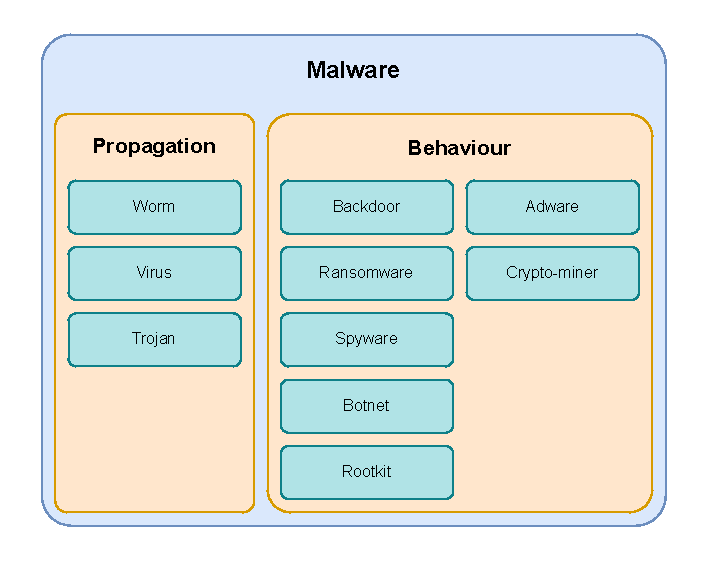
\includegraphics[width=0.5\textwidth]{malware-taxonomy.pdf}
        \caption{The different types of malware, based on their behavior and method of spread}
    \end{figure}
\end{frame}
}

\begin{frame}{Malware}
    \begin{block}{Definition}
        \textbf{Malware} --- Software that has a harmful effect on the typical operation of a host system.\footcite{kramerGeneralDefinitionMalware2010a}
    \end{block}

    \begin{itemize}
        \item Provides unauthorised access 
        \item Allows extraction or modification of information
        \item Prevents authorised users from accessing it 
    \end{itemize}
\end{frame}

{\nologo
\begin{frame}{Malware}{Obfuscation}
    \begin{figure}[htbp]
        \centering
        \begin{subfigure}[b]{0.45\textwidth}
            \centering
            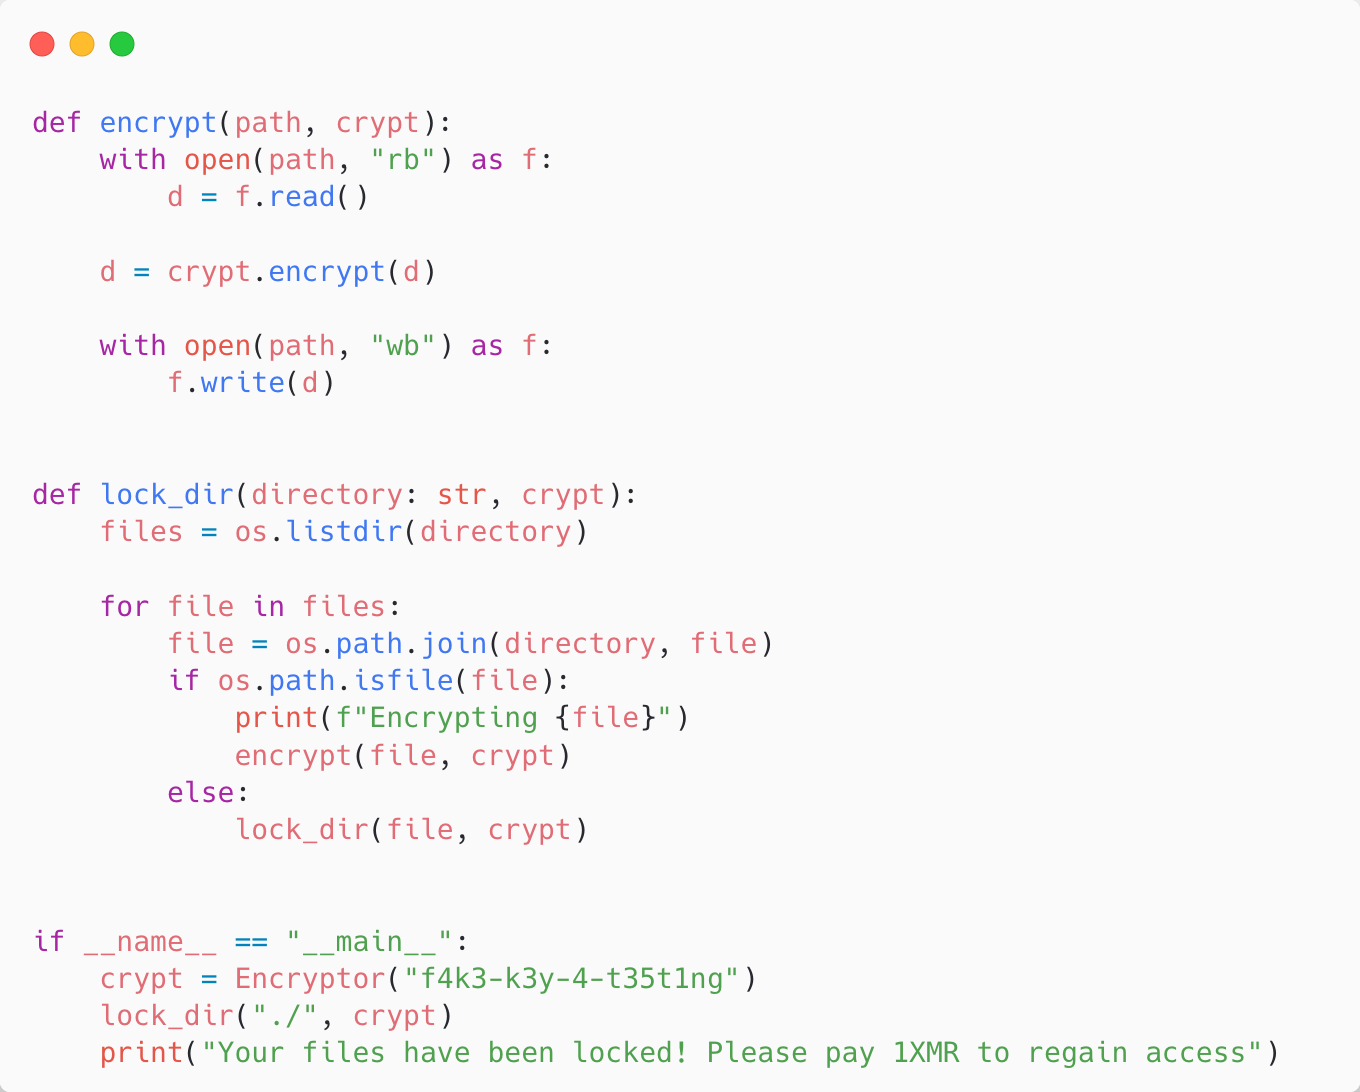
\includegraphics[width=0.75\textwidth]{malware-unobf.png}
            \caption{Before}
        \end{subfigure}
        \hfill 
        \begin{subfigure}[b]{0.45\textwidth}
            \centering
            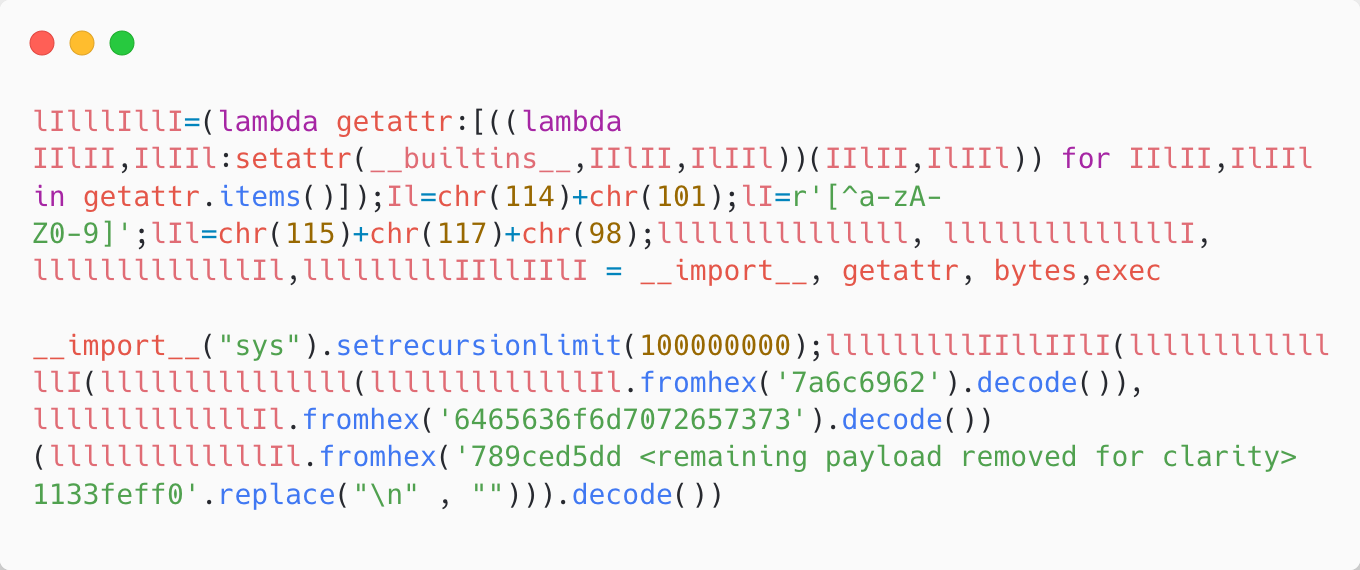
\includegraphics[width=0.75\textwidth]{malware-obfs.png}
            \caption{After}
        \end{subfigure}
        \caption{Ransomware shown before, and after obfuscation}
    \end{figure} 
\end{frame}
}


\section{Detection}

\begin{frame}{Malware Detection}{Types}
    \begin{itemize}
        \item \textbf{Static} --- File structure 

        \begin{itemize}
            \item Metadata 
            \item Byte sequences 
            \item Cryptographic hash 
        \end{itemize}

        \item \textbf{Dynamic} --- Behavioral characteristics
        
        \begin{itemize}
            \item API call sequences
            \item System modifications 
            \item Network communication
        \end{itemize}

        \item \textbf{Hybrid} --- Mix of static and dynamic features
    \end{itemize} 
\end{frame}

\begin{frame}{Our Approach}{Dataset}
    \begin{itemize}
        \item Lack of suitable datasets 
        \begin{itemize}
            \item EMBER\footcite{andersonEMBEROpenDataset2018} \& BODMAS\footcite{yangBODMASOpenDataset2021} do not distribute executables
            \item Others do not distribute benign executables
        \end{itemize}
        \item Malicious samples from VirusShare 

        \begin{itemize}
            \item Large scale database of malware seen in the wild 
            \item $>$ 100 million samples
        \end{itemize}

        \item Benign samples from my personal system 

        \begin{itemize}
            \item Video games 
            \item Developer tools 
            \item Custom software 
            \item Pre-installed programs (system executables, internet browser, etc.)
            \item Verified benign with windows defender
            \item Approx. 5000 in total
        \end{itemize}
    \end{itemize}    
\end{frame}

\begin{frame}{Our Approach}{Dataset --- Obfuscation}
    \begin{itemize}
        \item Obfuscation is more pervasive in malicious software 
        \item Analysis coverage --- ratio of the amount of code analysed to its total amount in a program 
        \item Coverage is typically lower in obfuscated programs
        \item \emph{Do static approaches learn to identify obfuscation as an indicator of malware?}
    \end{itemize}
\end{frame}

\begin{frame}{Our Approach}{Dataset --- Obfuscation}
    \begin{figure}
        \centering
        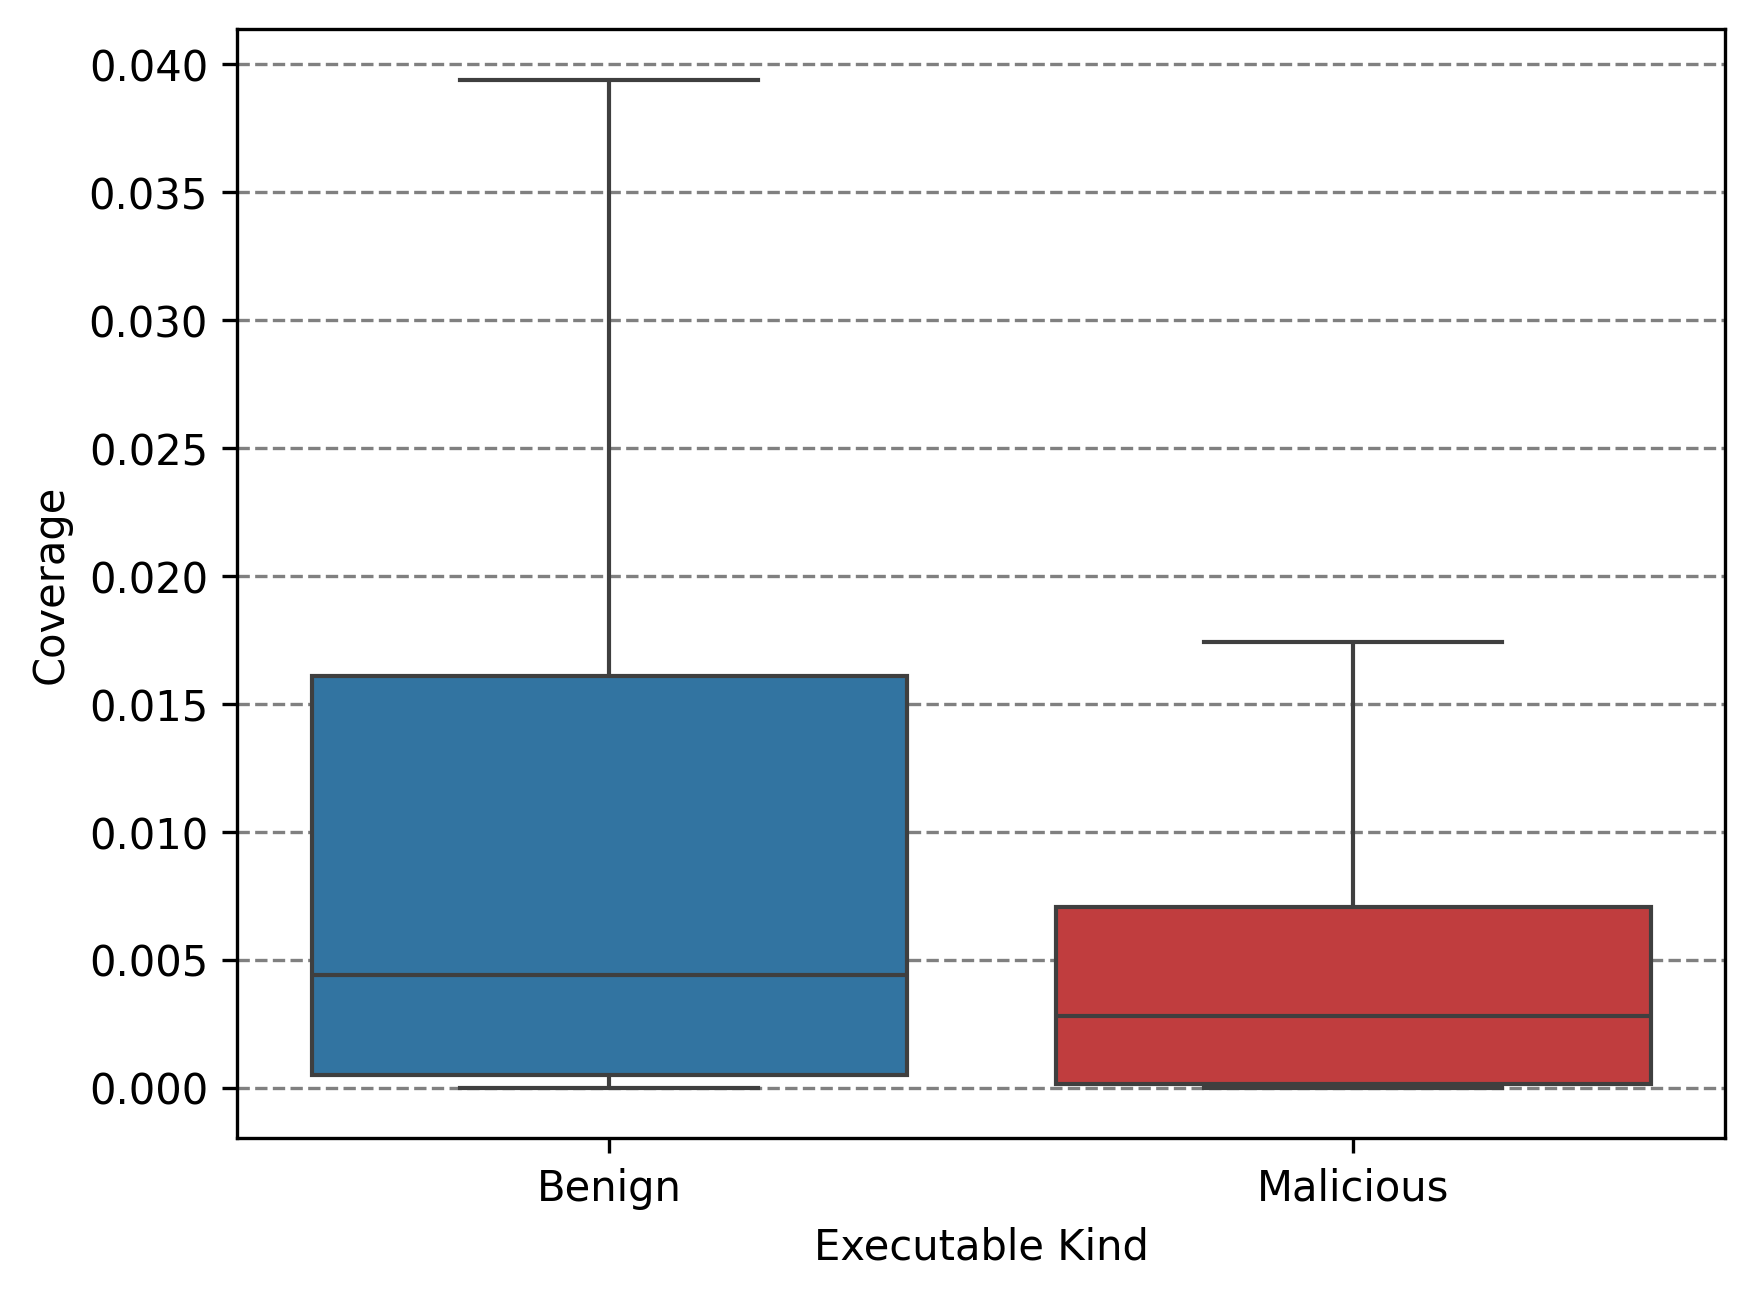
\includegraphics[width=0.7\textwidth]{obfuscation-dist.png}
        \caption{Code analysis coverage of the malicious and benign executables in our dataset}
    \end{figure} 
\end{frame}

\begin{frame}{Our Approach}{Models}
    \begin{itemize}
        \item Sequence-based 

        \begin{itemize}
            \item Identify malicious instruction sequences, aggregate sequence level classification across the file.
            \item BERT architecture\footcite{devlinBERTPretrainingDeep2019a} 
            \item Pretraining? 
        \end{itemize}

        \item Image-based 

        \begin{itemize}
            \item Convert programs to images 
            \item Identify malicious image-representations 
            \item EfficientNet B0 architecture\footcite{tanEfficientNetRethinkingModel2020}
        \end{itemize}
    \end{itemize} 
\end{frame}

\begin{frame}{Our Approach}{Sequence Classification}
    \begin{figure}
        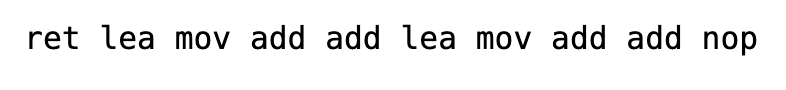
\includegraphics[width=0.8\textwidth]{opcode-sequence.png}
        \caption{A sequence of opcodes used by our model}
    \end{figure}
    \begin{itemize}
        \item Hyperparameter sweep to identify best architecture configuration 
        \item Does pre-training on Masked Language Modelling help? 
        \item Can we only train the classification head for this problem? 
    \end{itemize}
\end{frame}

\begin{frame}{Our Approach}{Sequence Classification --- Architecture}
\begin{table}[h]
    \centering
    \caption{BERT sequence classification model parameters}
    \begin{tabular}{@{}lr@{}}
        \toprule
        \textbf{Parameter}      & \textbf{Value} \\ \midrule
        Sequence Length         & 32    \\
        Hidden Layer Size       & 512   \\
        Hidden Layers           & 7     \\
        Attention Heads         & 4     \\
        Intermediate Layer Size & 2048  \\
        Activation Function     & GELU  \\
        Hidden Dropout Rate     & 0.01  \\
        Attention Dropout Rate  & 0.001 \\ \bottomrule
    \end{tabular}
    \label{tab:model-params}
\end{table}
\end{frame}

{\nologo
\begin{frame}{Our Approach}{Image Classification}
    \begin{figure}
        \centering 
        \begin{subfigure}{0.45\textwidth}
            \centering 
            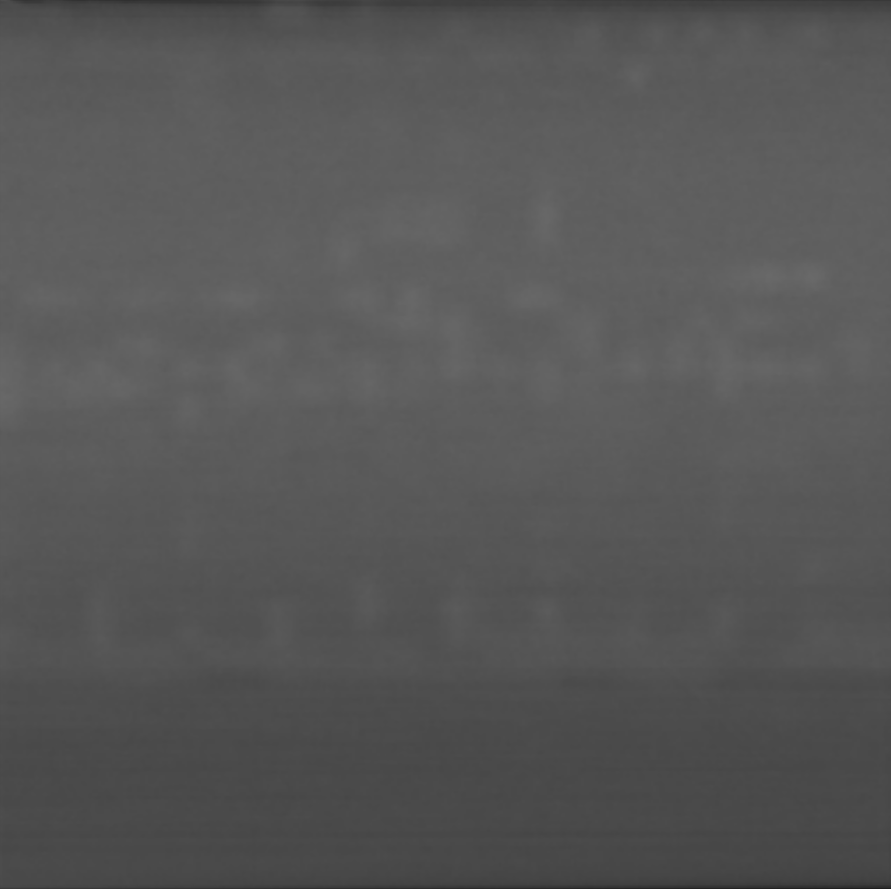
\includegraphics[width=0.5\textwidth]{avg-benign.png} 
            \caption{Benign}
        \end{subfigure}
        \hfill
        \begin{subfigure}{0.45\textwidth}
            \centering 
            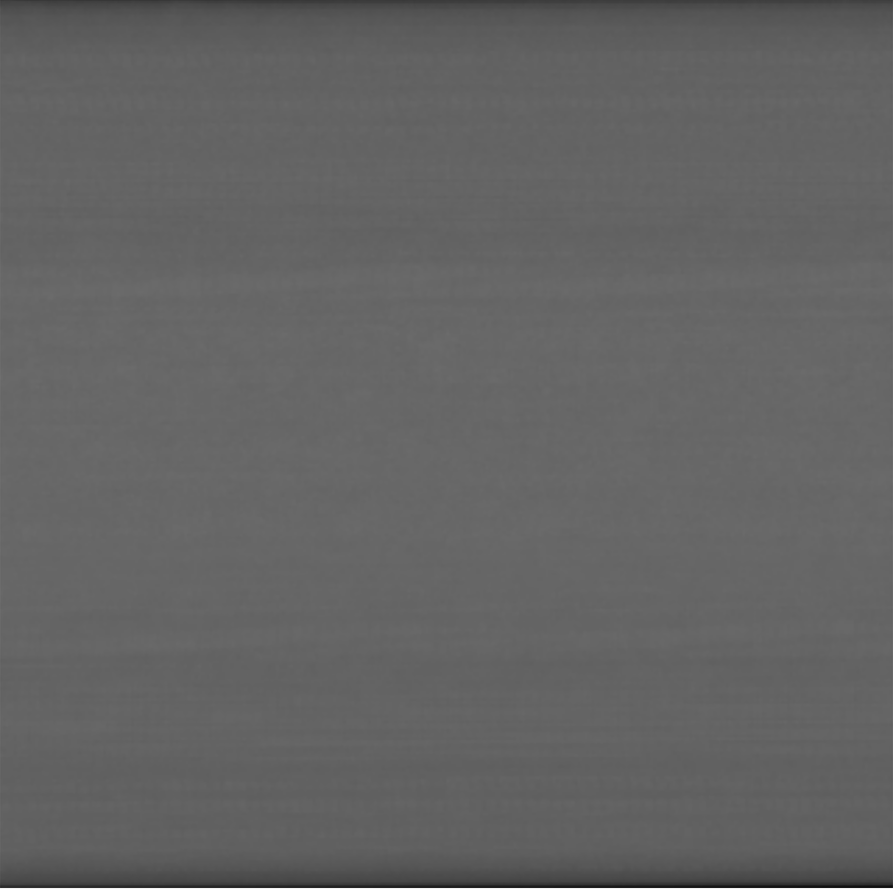
\includegraphics[width=0.5\textwidth]{avg-malicious.png} 
            \caption{Malicious}
        \end{subfigure}
        \caption{Average image representation of each class}
        \label{fig:img-rep}
    \end{figure}

    \begin{itemize}
        \item Malicious programs are often much smaller than benign programs 
        \item Benign programs are resized more than malicious programs 
        \item Does this model use scaling artifacts to distinguish between malicious and benign? 
    \end{itemize} 
\end{frame}
}

\begin{frame}{Our Approach}{Image Classification --- Size Distribution}
    \begin{figure}
        \centering 
        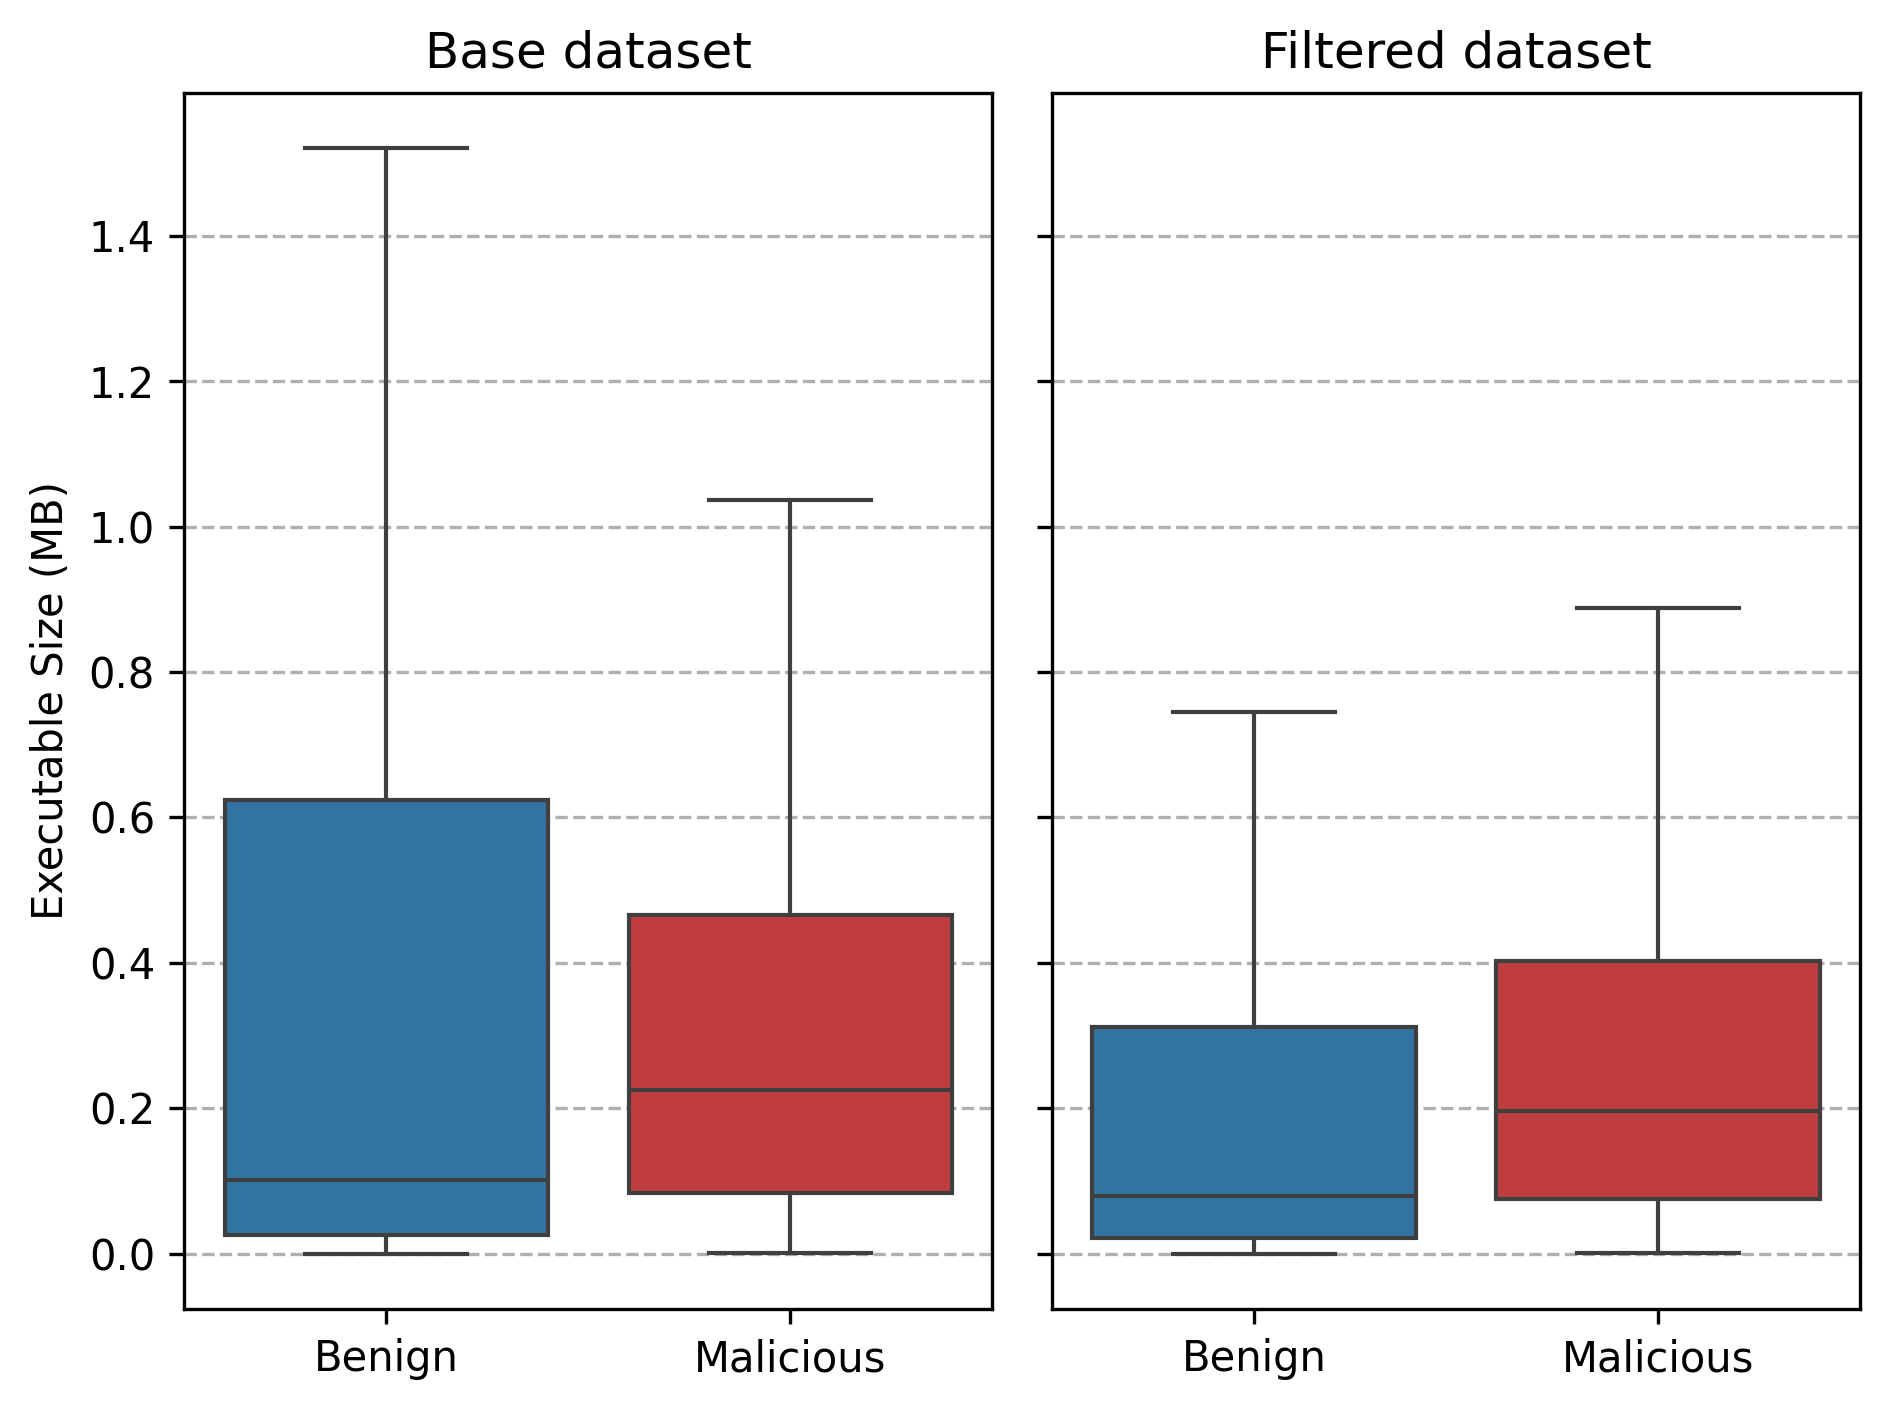
\includegraphics[width=0.5\textwidth]{filtered-dataset-size-comparison.png} 
        \caption{Comparison between the program size distribution for each class in our base dataset, and the filtered dataset} 
    \end{figure}    
\end{frame}

\section{Results}
{\nologo
\begin{frame}{Results}{Baseline}
   \begin{table}[h]
    \centering
    \caption{Performance of baseline methods for malware detection using the import tables of executables}
    \resizebox{\textwidth}{!}{%
    \begin{tabular}{llllll}
        \toprule
        \textbf{Algorithm} & \textbf{Feature} & \textbf{Accuracy} & \textbf{F1 Score} & \textbf{Precision} & \textbf{Recall} \\ \midrule
        \multirow{2}{*}{\textbf{Support Vector Classifier}} & DLL & 0.8859 & 0.8856 & 0.8856 & 0.8856 \\
        & Function & 0.9248 & 0.9248 & 0.9266 & 0.9262 \\ \midrule
        \multirow{2}{*}{\textbf{Logistic Regression}} & DLL & 0.8682 & 0.8682 & 0.8687 & 0.8695 \\
        & Function & 0.9438 & 0.9438 & 0.9442 & 0.9447 \\ \midrule
        \multirow{2}{*}{\textbf{Decision Tree}} & DLL & 0.8877 & 0.8876 & 0.8876 & 0.8885 \\
        & Function & 0.9406 & 0.9406 & 0.9415 & 0.9417 \\ \bottomrule
    \end{tabular}%
    }
    \label{tab:baseline-results}
    \end{table}
\end{frame}}

\begin{frame}{Results}{Sequence Classification}

\begin{table}[h]
    \centering
    \caption{Performance of our RoBERTa model for opcode sequence classification and malware detection}
    \resizebox{\textwidth}{!}{%
    \begin{tabular}{llllllllllll}
        \toprule
        \multicolumn{1}{c}{\multirow{2}{*}{\textbf{Model}}} &  & \multicolumn{4}{c}{\textbf{Sequence Level}} & \multicolumn{1}{c}{} & \multicolumn{4}{c}{\textbf{File Level}} & \vspace{2pt}\\ \cline{3-6} \cline{8-11}
        \multicolumn{1}{c}{} &  & Accuracy & F1-Score & Precision & Recall & \textbf{} & Accuracy & F1-Score & Precision & Recall &  \\  \midrule
        From Scratch &  & 0.8756 & 0.8742 & 0.8798 & 0.8756 &  & 0.8976 & 0.8971 & 0.9095 & 0.8989 &  \\
        From pretrained &  & 0.9010 & 0.9002 & 0.9042 & 0.9010 &  & 0.9452 & 0.9452 & 0.9479 & 0.9458 &  \\
        \begin{tabular}[c]{@{}l@{}}From pretrained \\ (w/ Frozen Attention Weights)\end{tabular} &  & 0.8302 & 0.8265 & 0.8409 & 0.8302 & & 0.8076 & 0.8037 & 0.8393 & 0.8098 &  \\ 
        \bottomrule
        \end{tabular}%
    }
    \label{tab:malberta-base-results}
\end{table}
\end{frame}


\begin{frame}{Results}{Image Classification}

\begin{table}[h]
    \centering
    \caption{Performance of the image classification models for malware detection}
    \begin{tabular}{@{}lllll@{}}
        \toprule
        \textbf{Dataset} & \textbf{Accuracy} & \textbf{F1-Score} & \textbf{Precision} & \textbf{Recall} \\ \midrule
        Full & 0.9316 & 0.9315 & 0.9314 & 0.9322 \\
        Filtered & 0.9306 & 0.9306 & 0.9309 & 0.9306 \\ \bottomrule
    \end{tabular}
    \label{tab:image-classifier-model-results}
\end{table}
\end{frame}



\begin{frame}{Results}{Sequence Classification --- Obfuscation}
    \begin{figure}
        \centering
        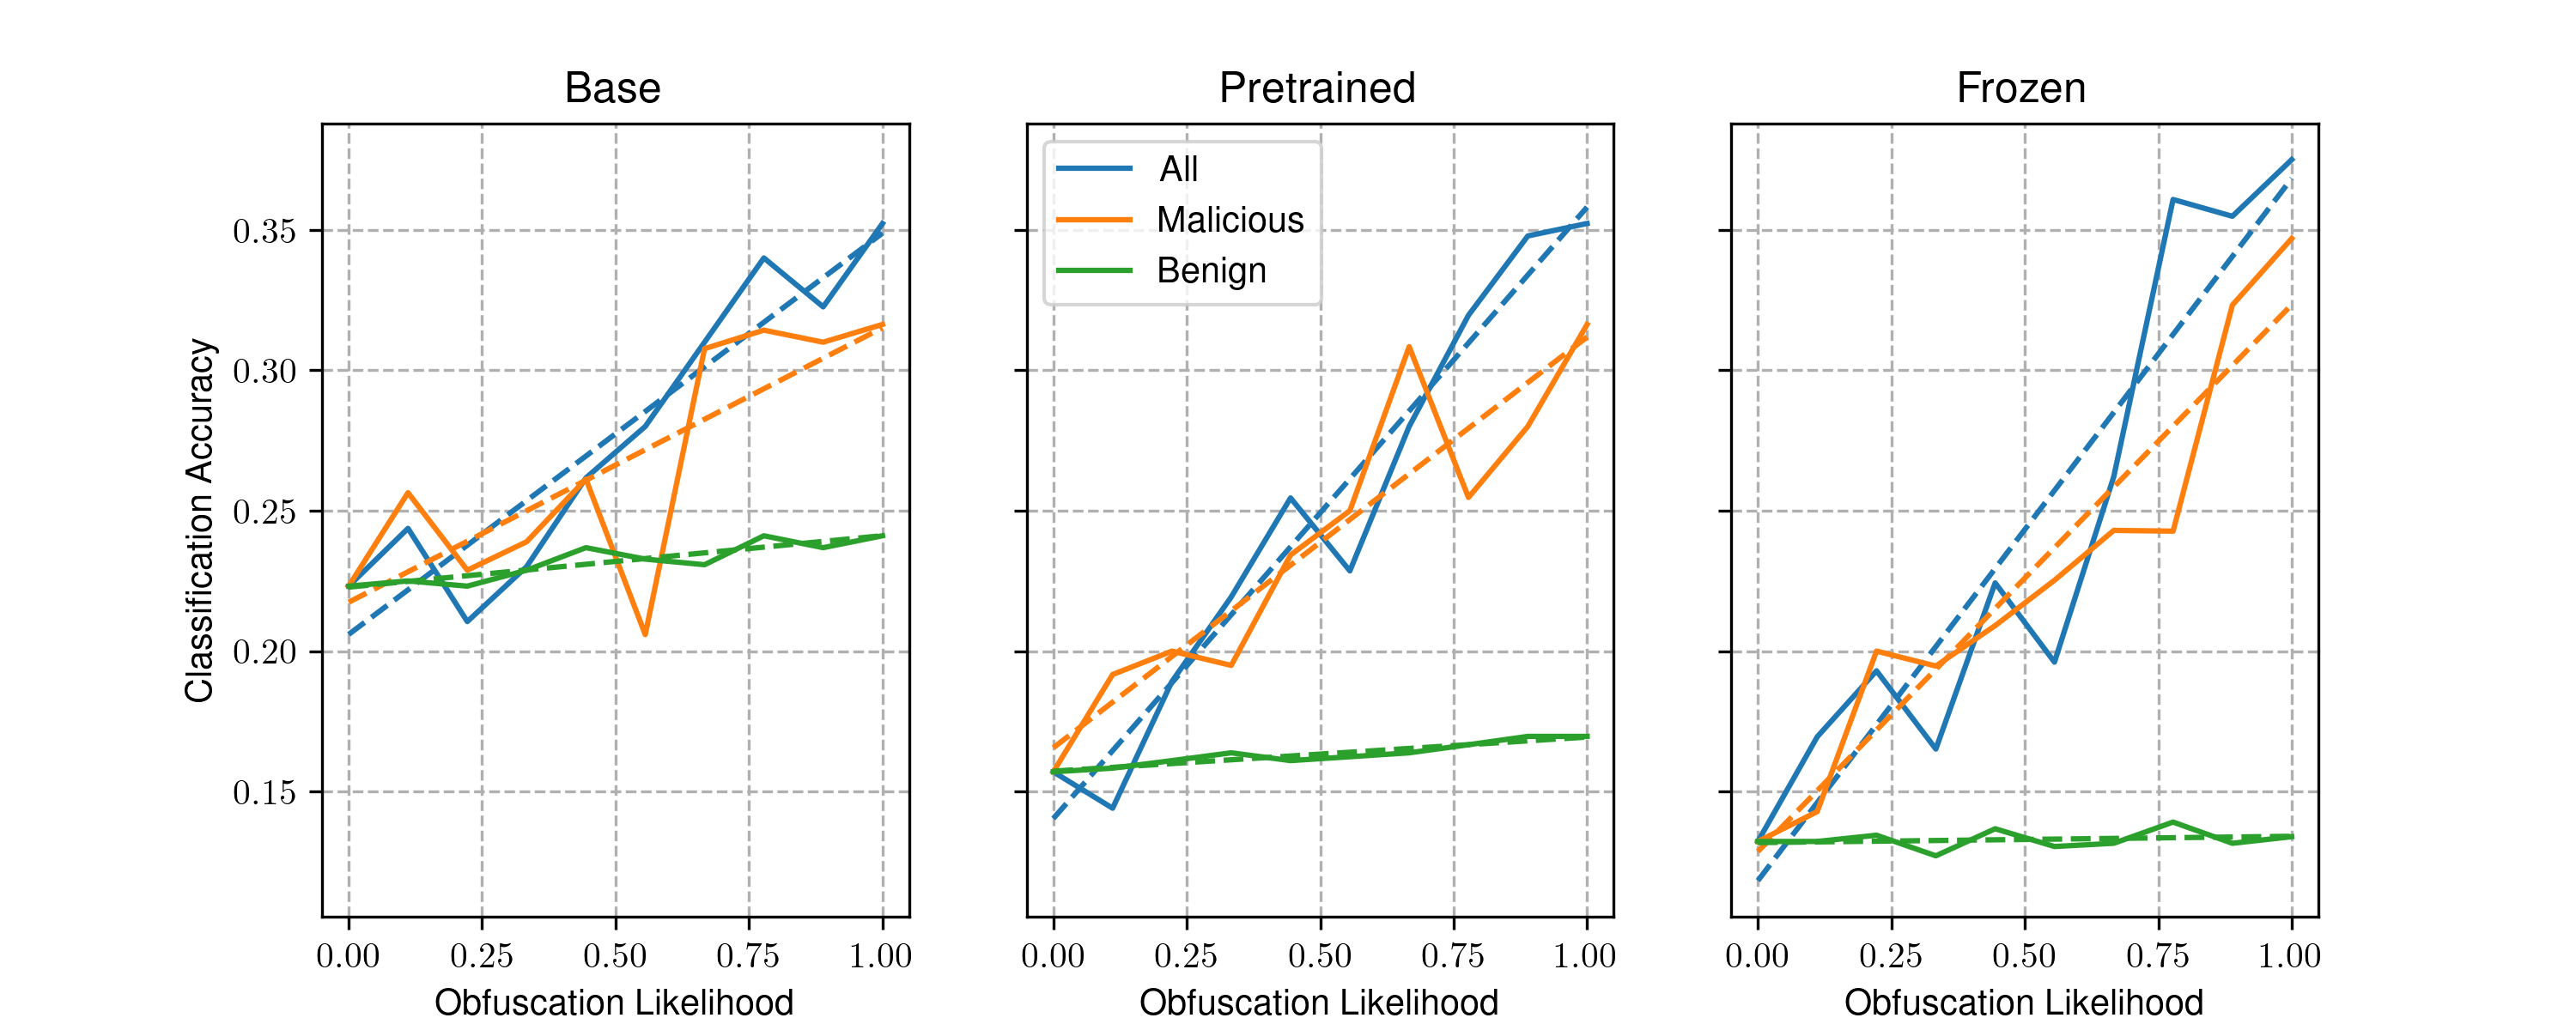
\includegraphics[width=\textwidth]{seq-obf-file-level-base.png}
        \caption{How obfuscation impacts the file level classification accuracy of our Sequence classification models.}
    \end{figure}
\end{frame}

\begin{frame}{Results}{Image Classification --- Obfuscation}
    \begin{figure}
        \centering
        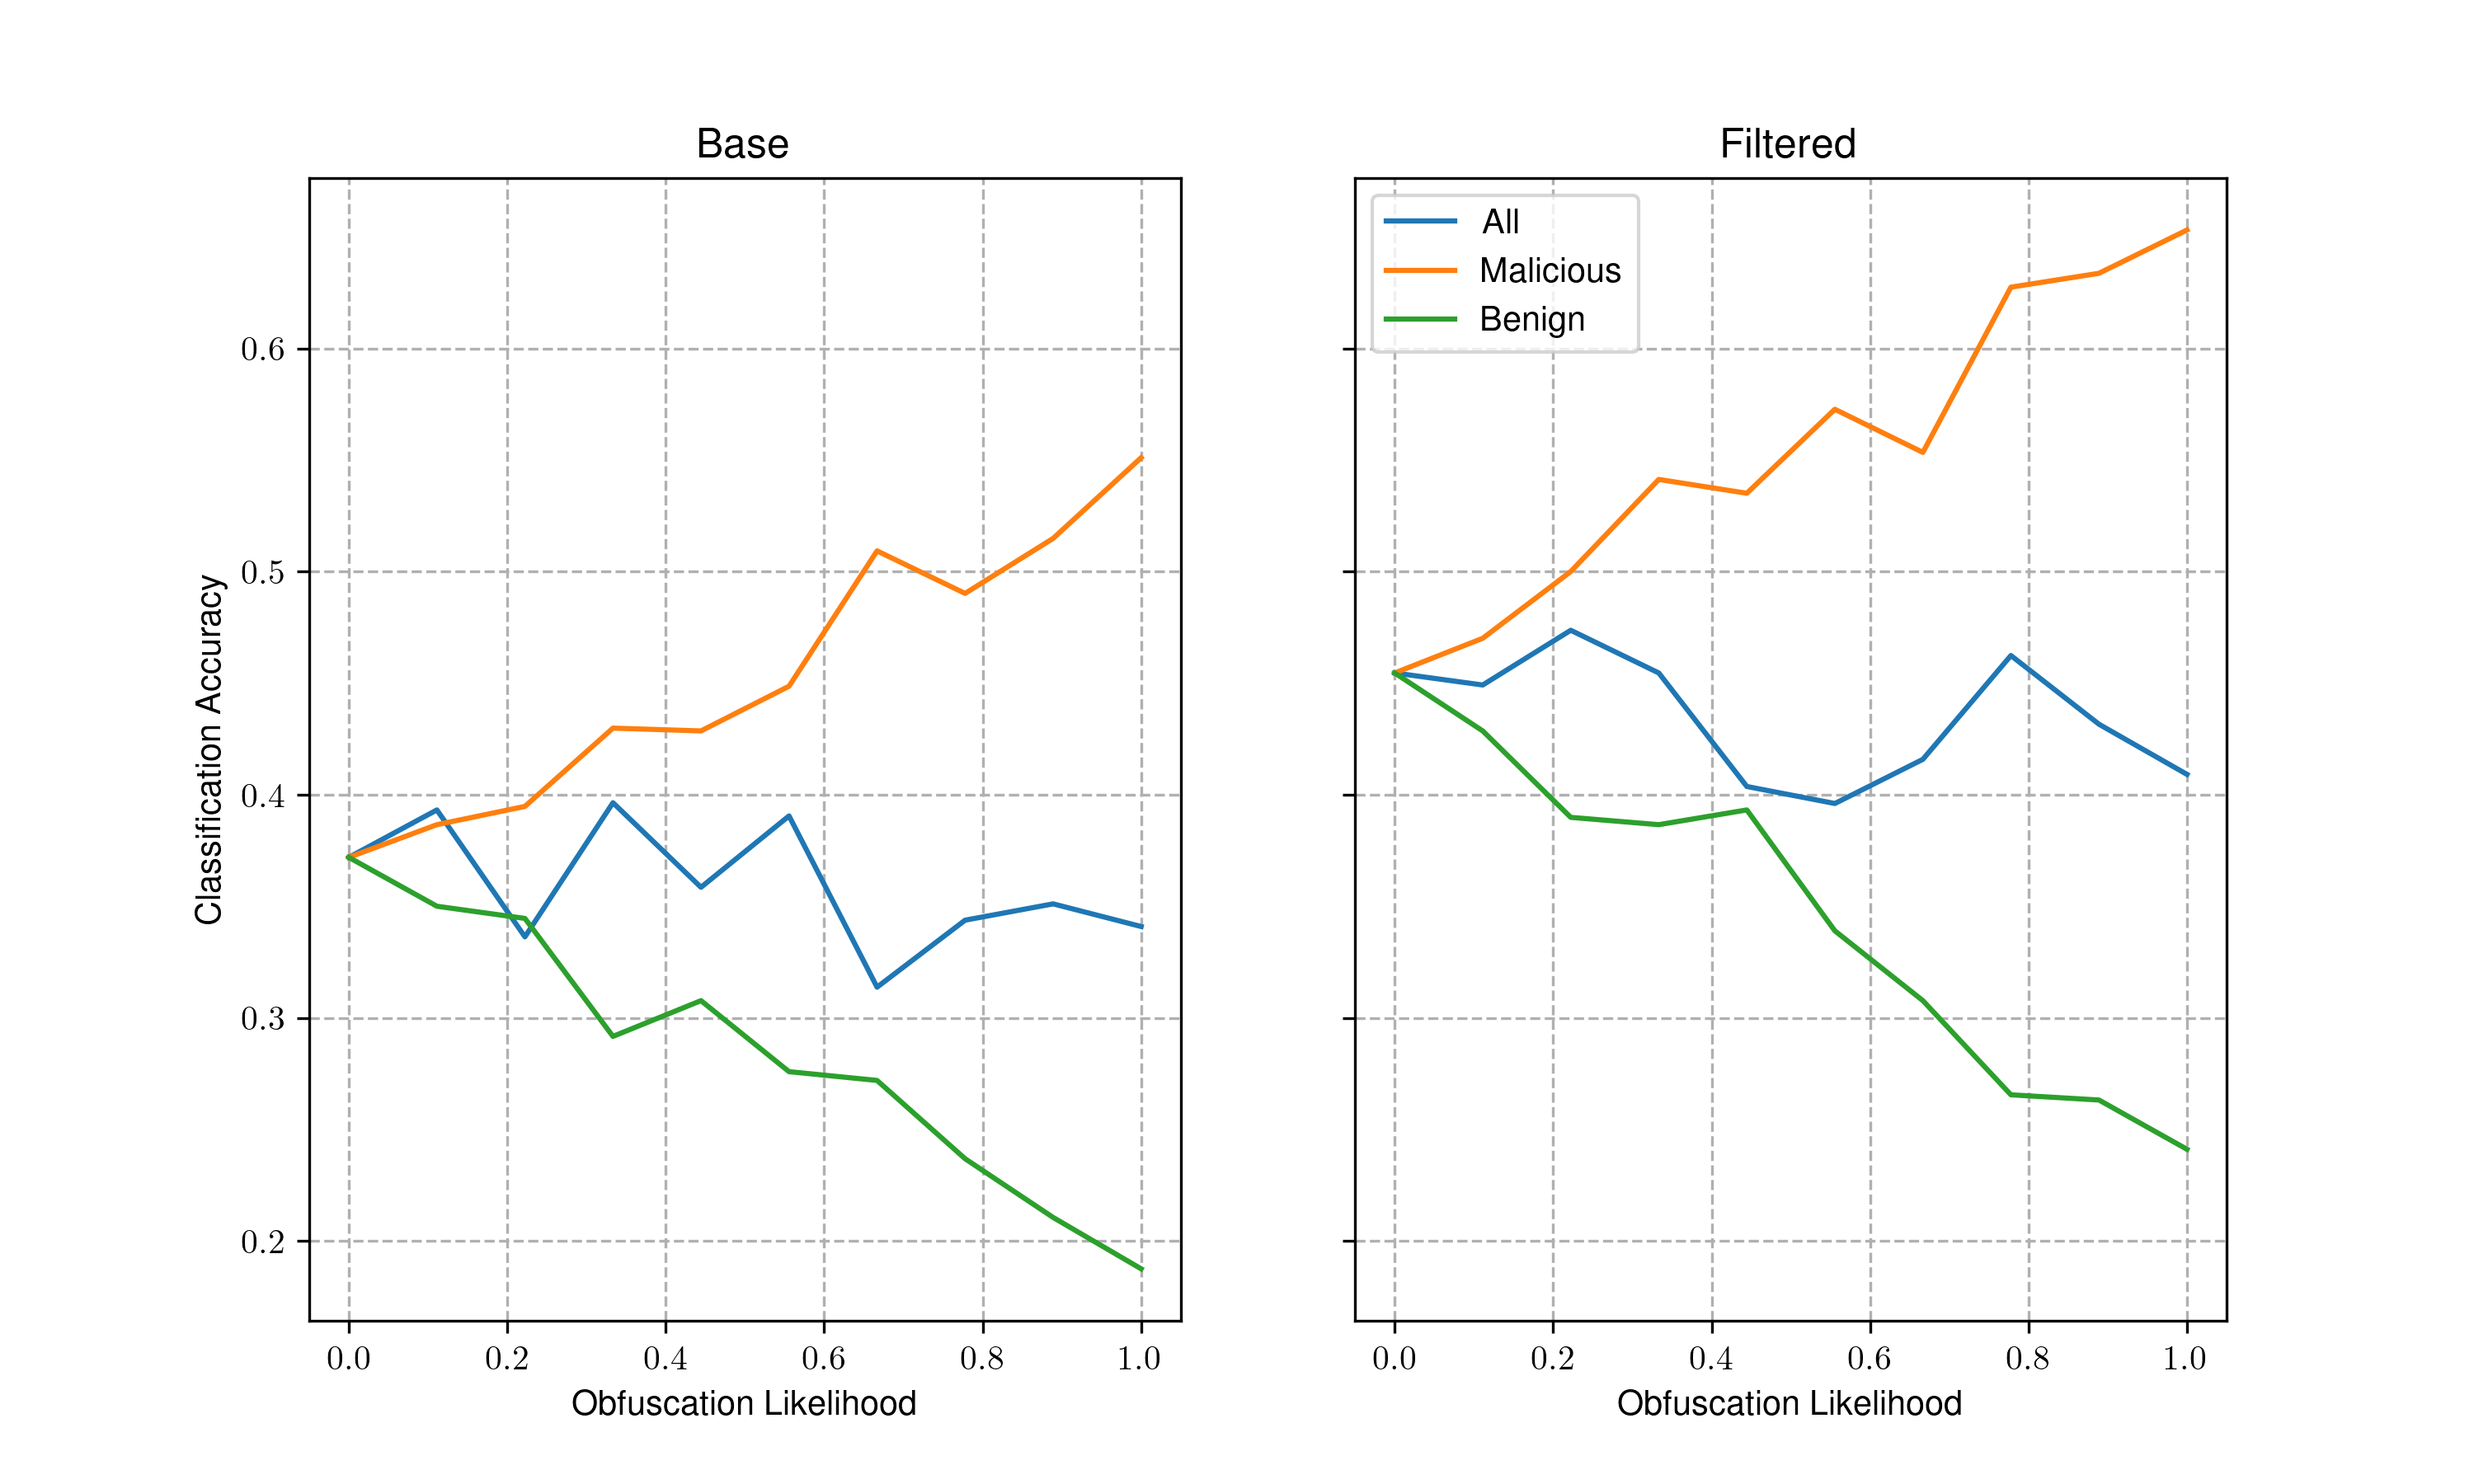
\includegraphics[width=0.7\textwidth]{img-obf-file-level.png}
        \caption{How obfuscation impacts the file level classification accuracy of our image classification models.}
    \end{figure}
\end{frame}

\section{Conclusion}

\begin{frame}{Conclusion}{Findings}
    \begin{itemize}
        \item Sequence classification model offers best performance overall 
        \item Image classification model does not surpass our baseline, and is highly reliant on obfuscation as an indicator of malware. 
        \item Sequence classification model is also reliant on obfuscation but to a lesser extent 
    \end{itemize} 
\end{frame}

\begin{frame}{Conclusion}{Limitations}
    \begin{itemize}
        \item Dataset limitations
        
        \begin{itemize}
            \item Coverage analysis in secondary dataset 
            \item Significant performance disparity between primary and seondary dataset 
        \end{itemize}

        \item Choice of opcode sequences 
        
        \begin{itemize}
            \item Full disassembly for basic blocks? 
        \end{itemize}
    \end{itemize}
\end{frame}

\begin{frame}
    \vfill
    \begin{center}
        {\usebeamercolor[fg]{frametitle}\bfseries\LARGE Questions?}
    \end{center}
    \vfill
\end{frame}

\appendix 

{\nologo

\begin{frame}{Malware}{Impact}
    \begin{itemize}
        \item WannaCry 

        \begin{itemize}
            \item Infected 200,000 systems 
            \item \$4 billion
            \item Crippled the National Health Service 
        \end{itemize}

        \item Stuxnet
        
        \begin{itemize}
            \item Infected 60\% of all computers in Iran 
            \item Significantly impacted their ability to enrich nuclear material 
            \item First known example of a ``Cyber-Weapon''
        \end{itemize}
    \end{itemize}
\end{frame}

\begin{frame}{Opcode Extraction}
    \begin{figure}
        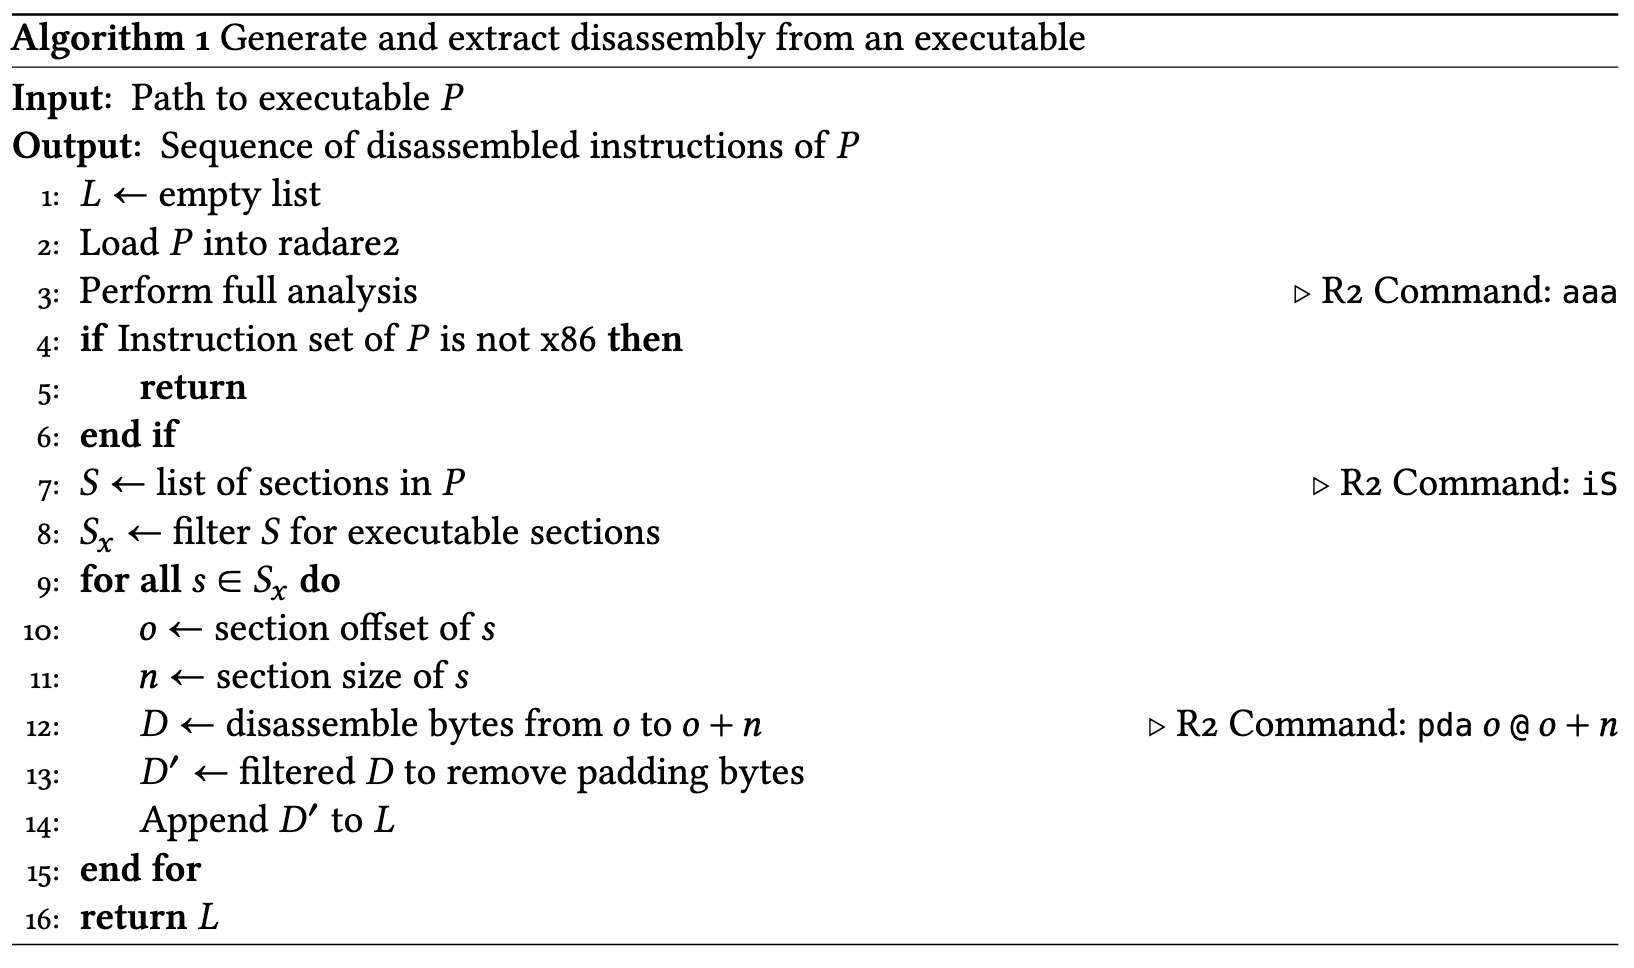
\includegraphics[width=0.9\textwidth]{opcode-extraction.png}
    \end{figure}
    
\end{frame}

\begin{frame}{Base Model}{F1 Score}
    \begin{figure}
        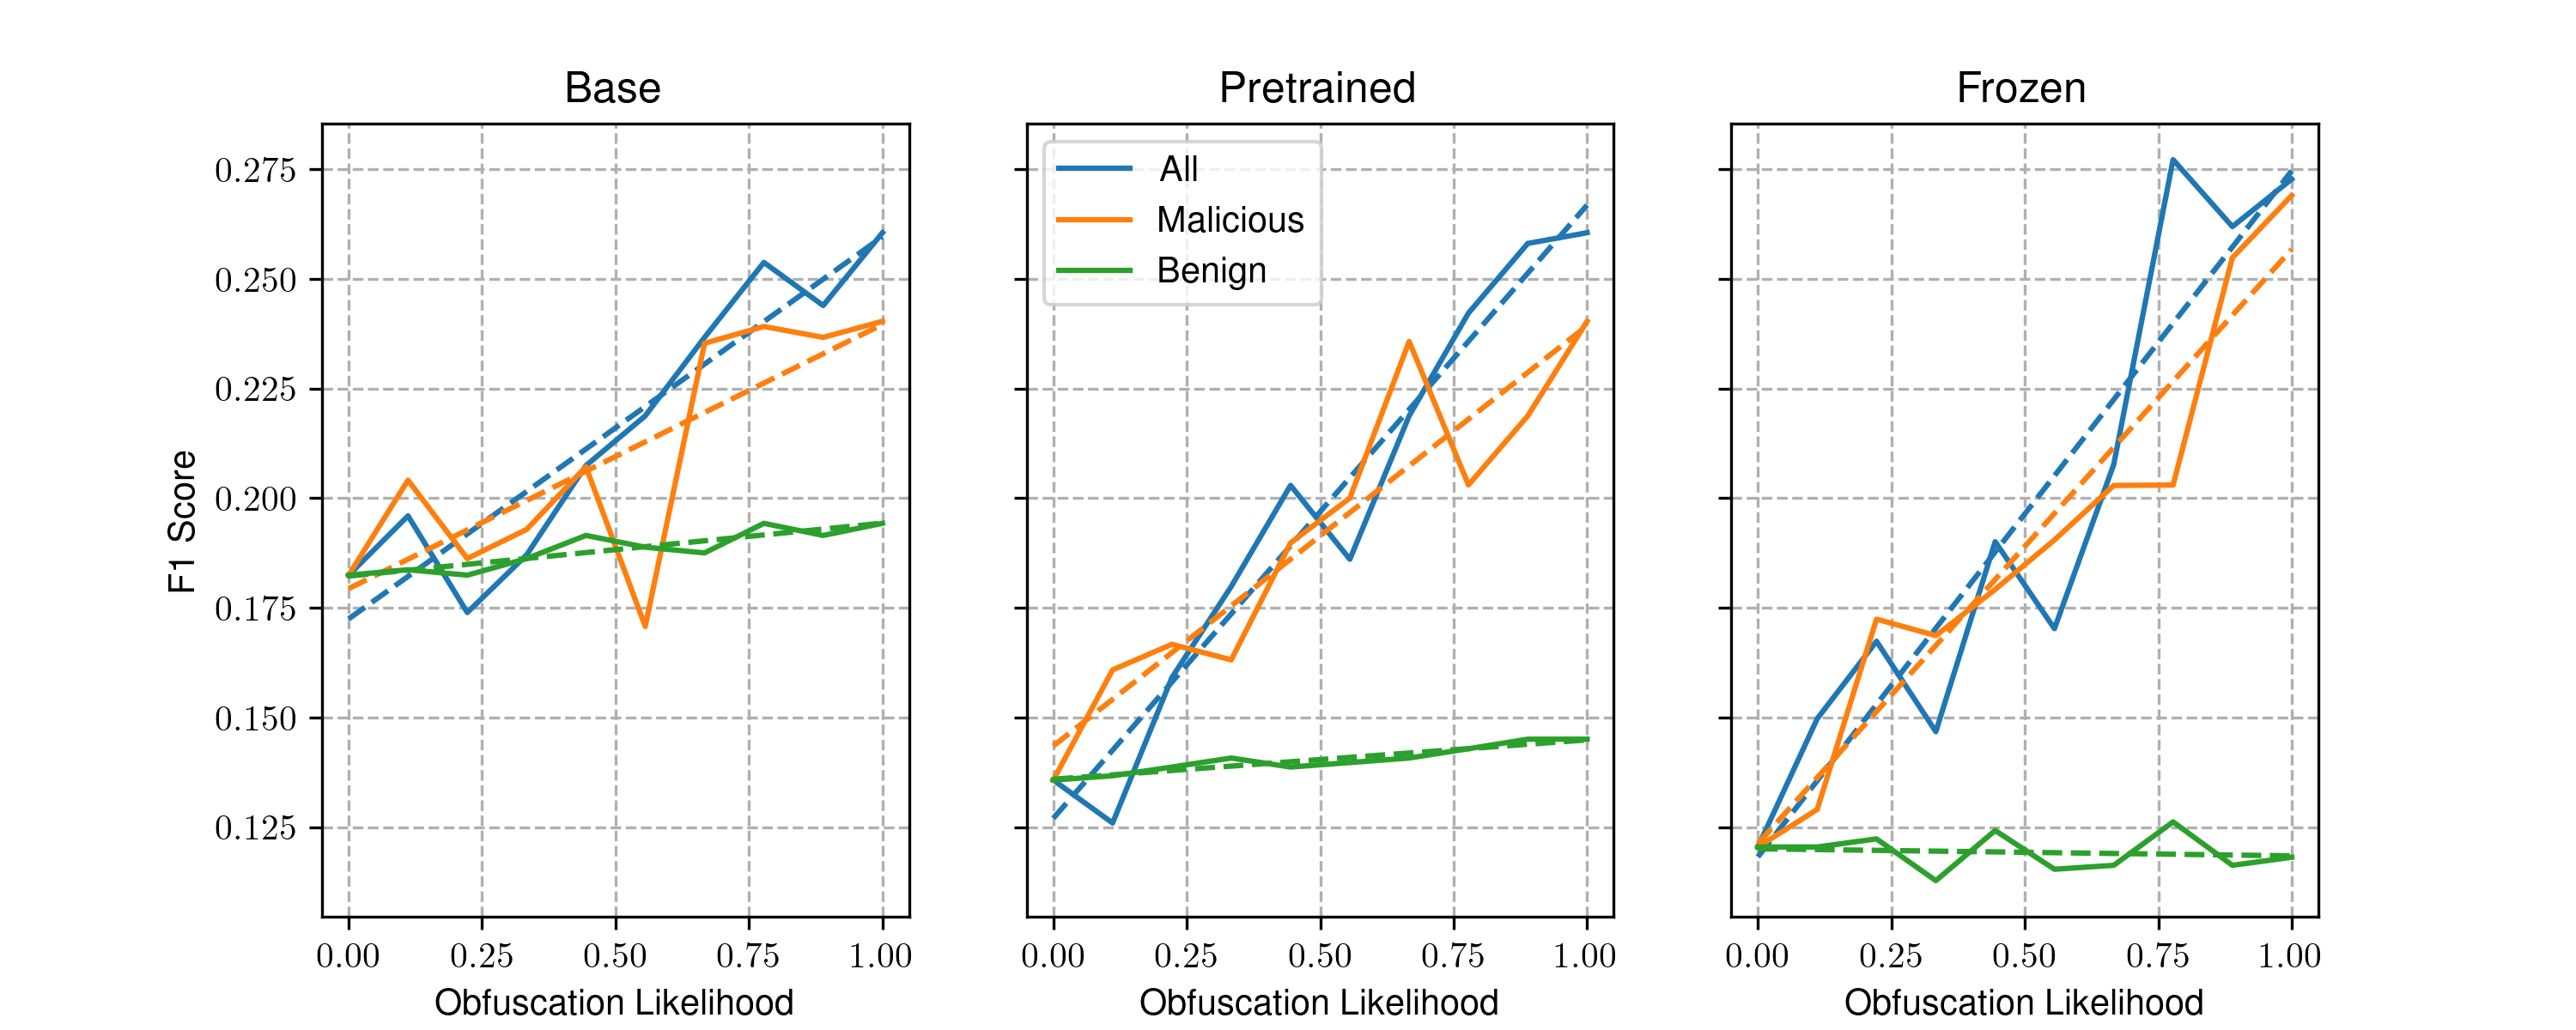
\includegraphics[width=\textwidth]{seq-obf-file-level-base-f1-score.png}
        \caption{File Level F1 score}
    \end{figure} 
\end{frame}

\begin{frame}{Base Model}{Sequence Accuracy}
    \begin{figure}
        
\includegraphics[width=\textwidth]{seq-obf-seq-level-base.png}
        \caption{Sequence-level performance}
    \end{figure} 
\end{frame}

\begin{frame}{Base Model}{Certainty}
    \begin{figure}
        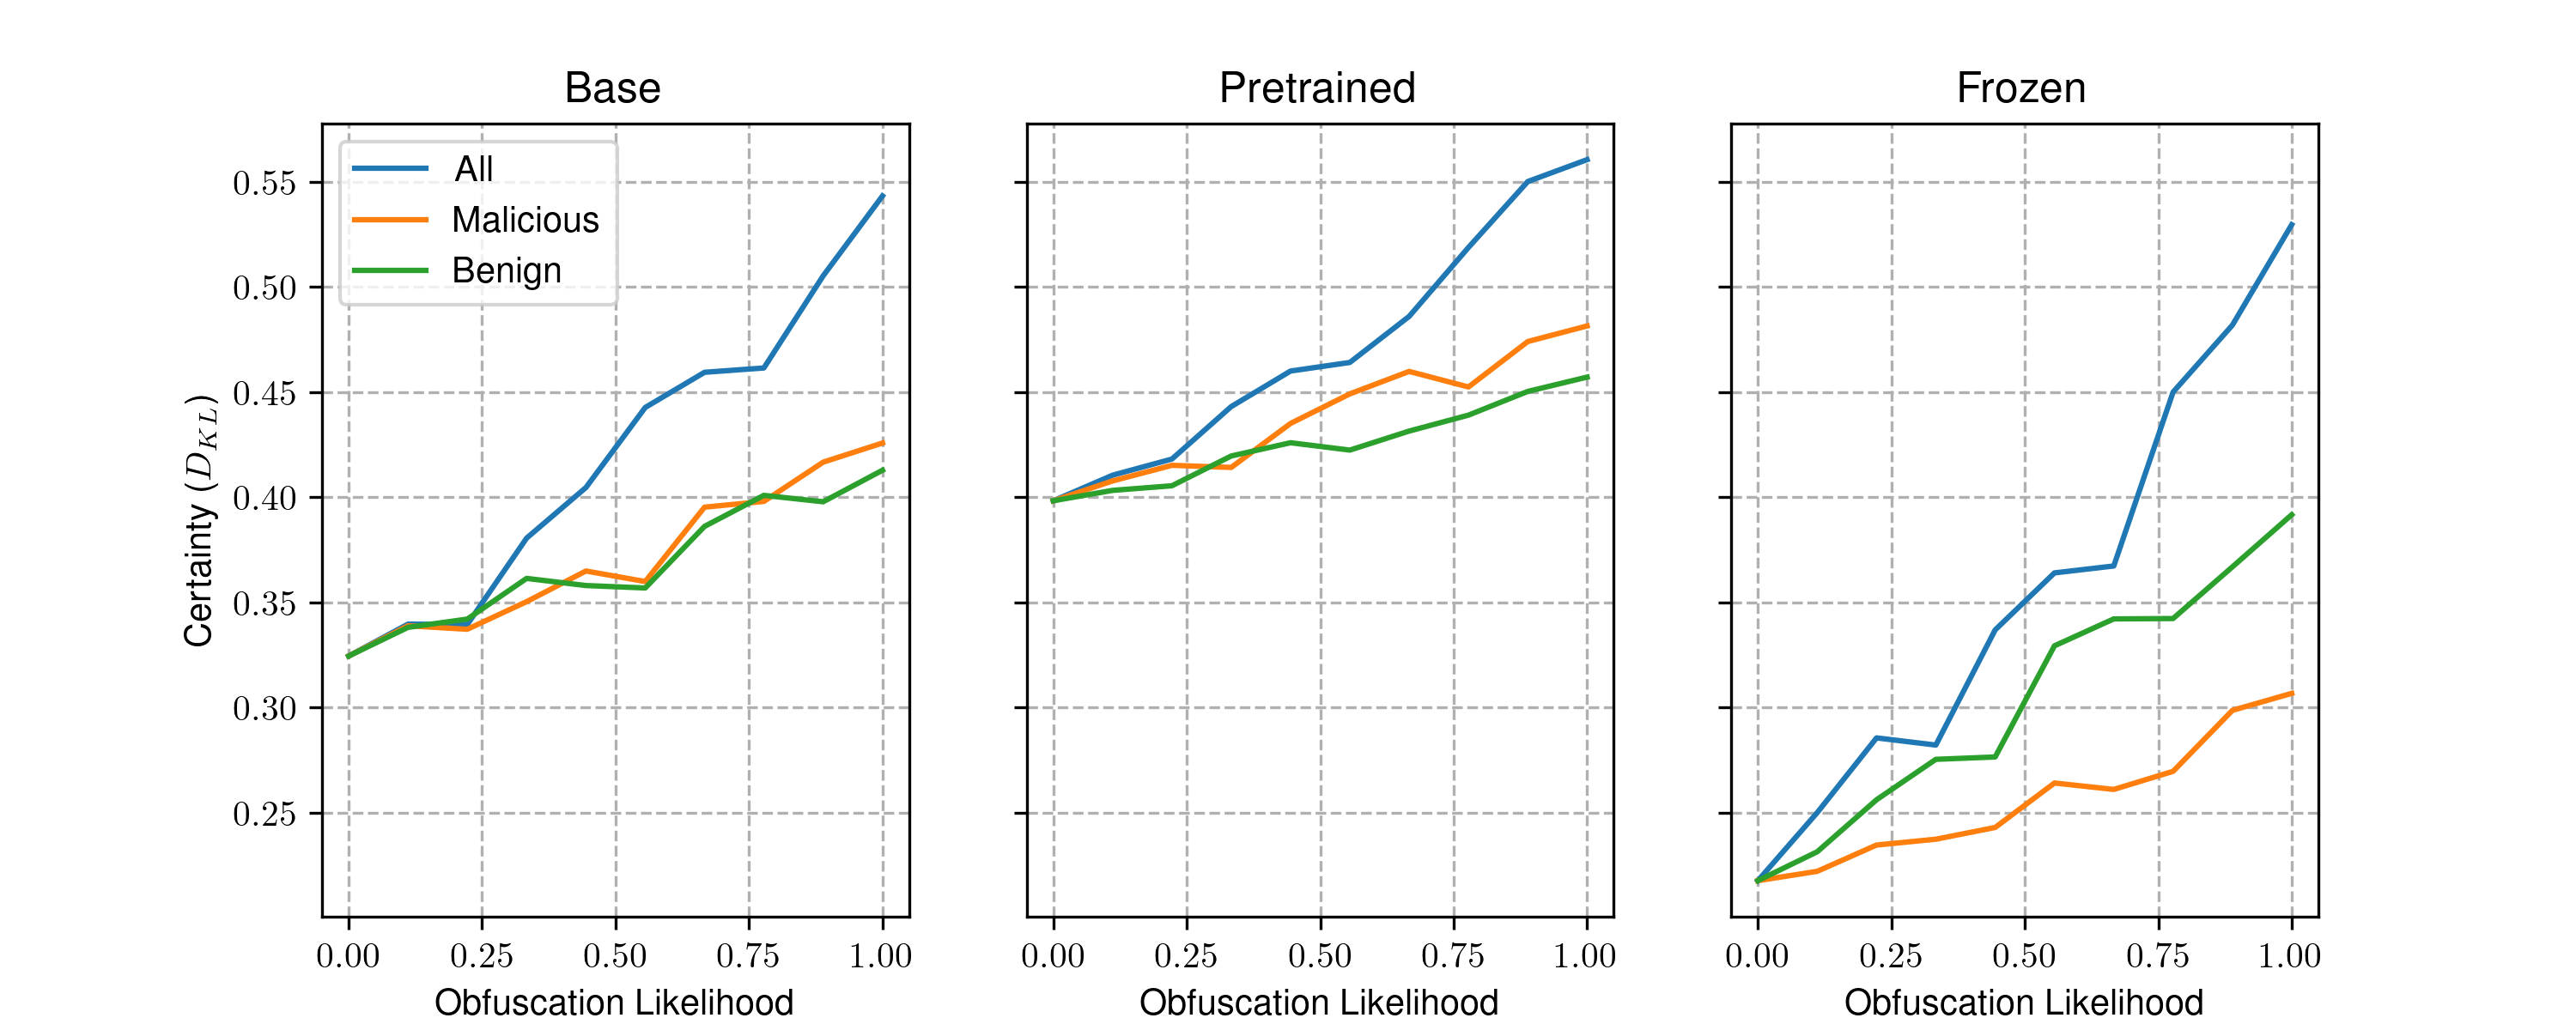
\includegraphics[width=\textwidth]{seq-obf-certainty-base.png}
        \caption{Confidence}
    \end{figure} 
\end{frame}

\begin{frame}{Base Model}{RSA of Pretrained and Non-Pretrained Models}
    \begin{figure}
        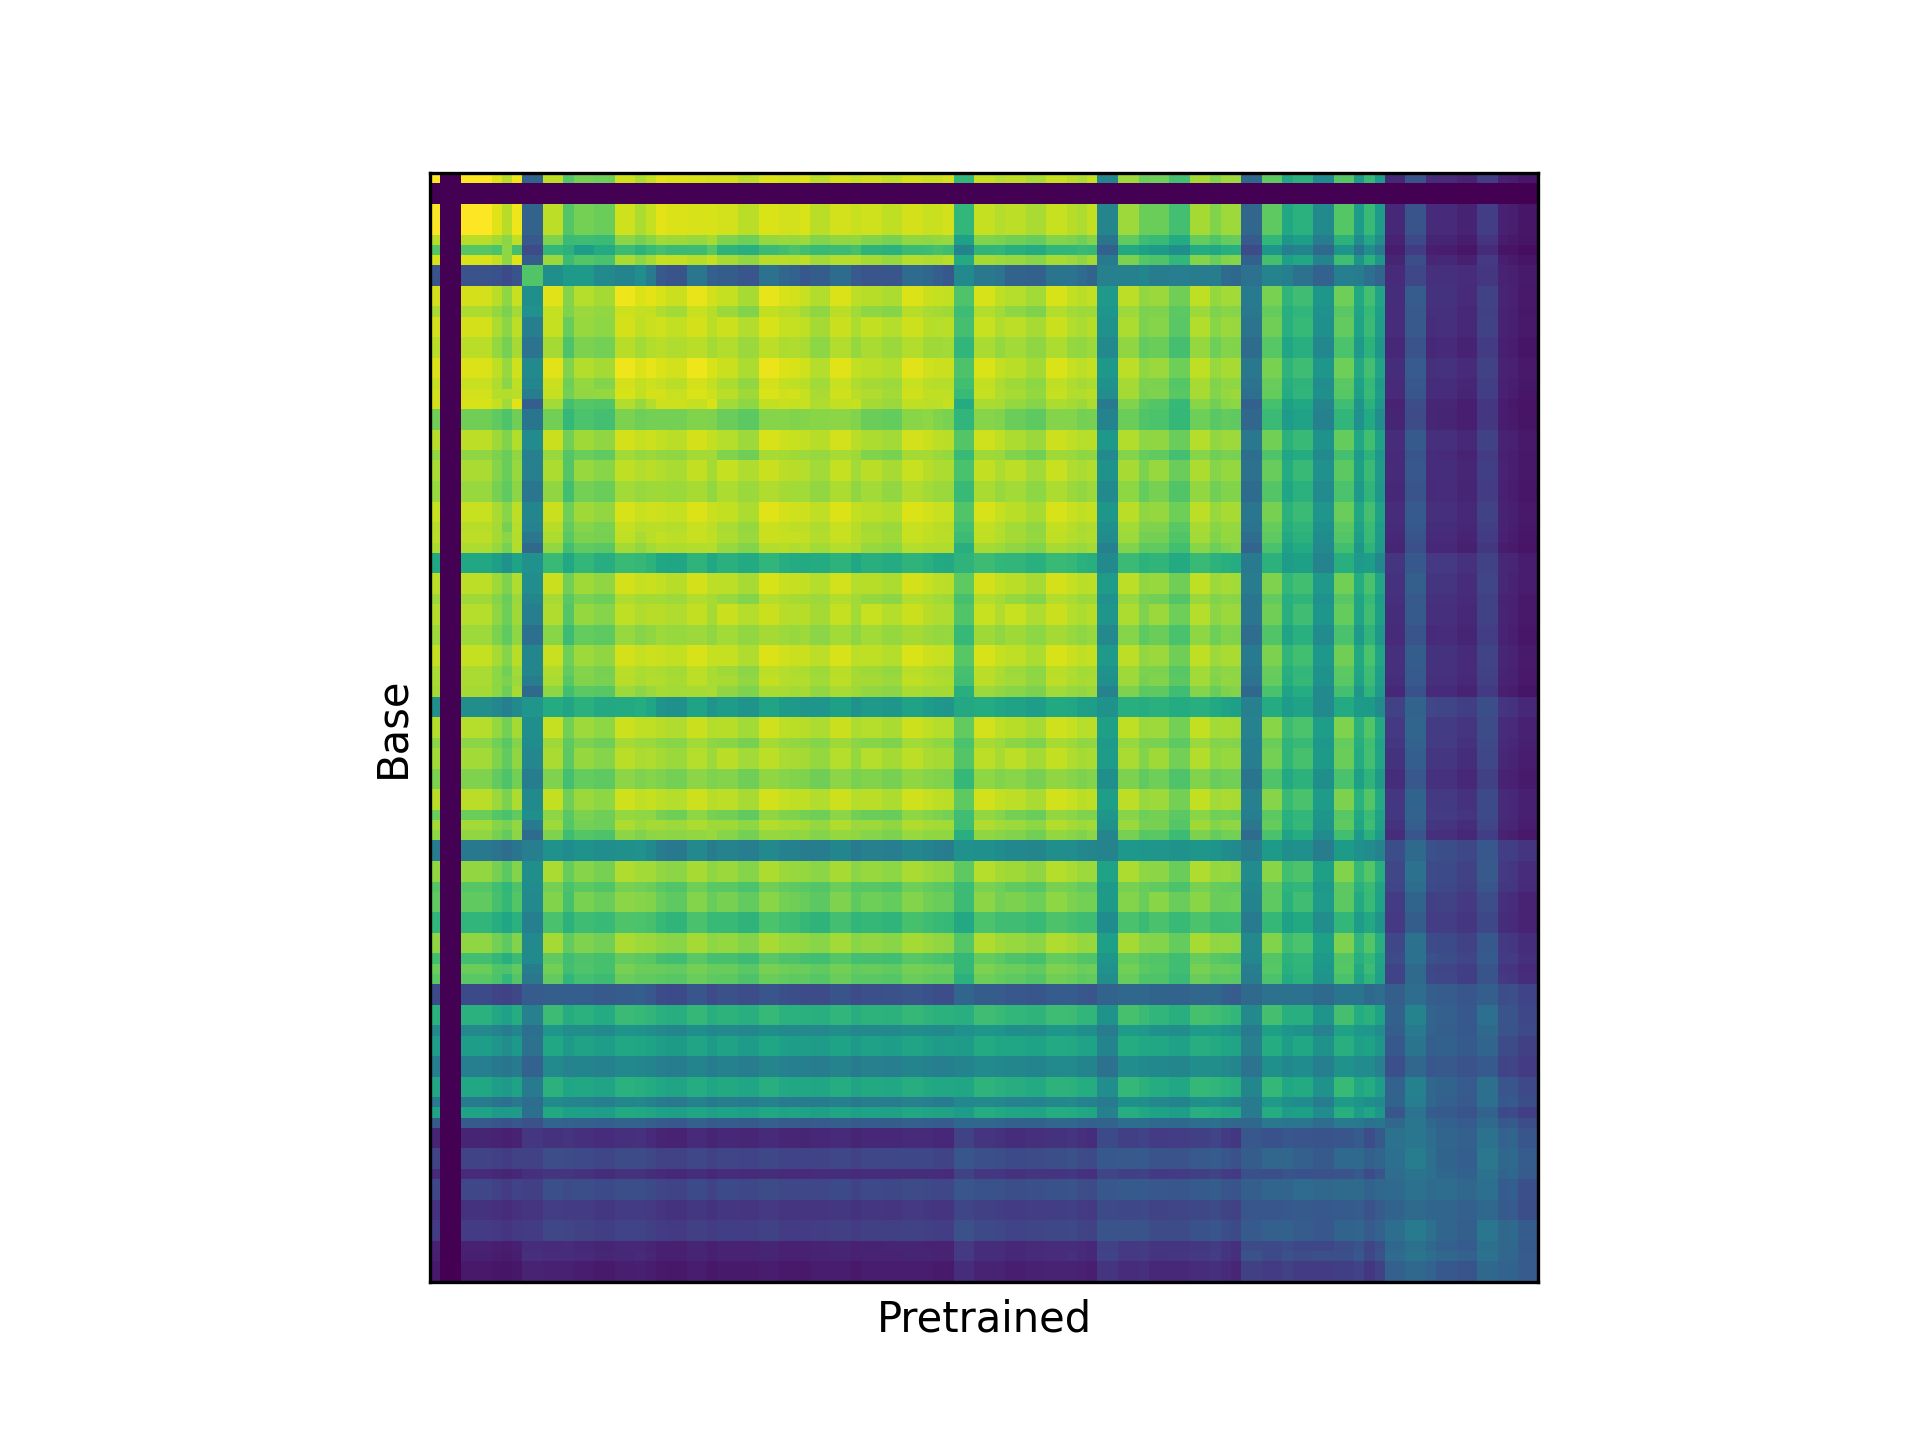
\includegraphics[width=0.5\textwidth]{rsa-cka-base-pretrained-scratch.png}
    \end{figure}
\end{frame}

\begin{frame}{Base Model}{RSA of Pretrained and Frozen Pretrained Models}
    \begin{figure}
        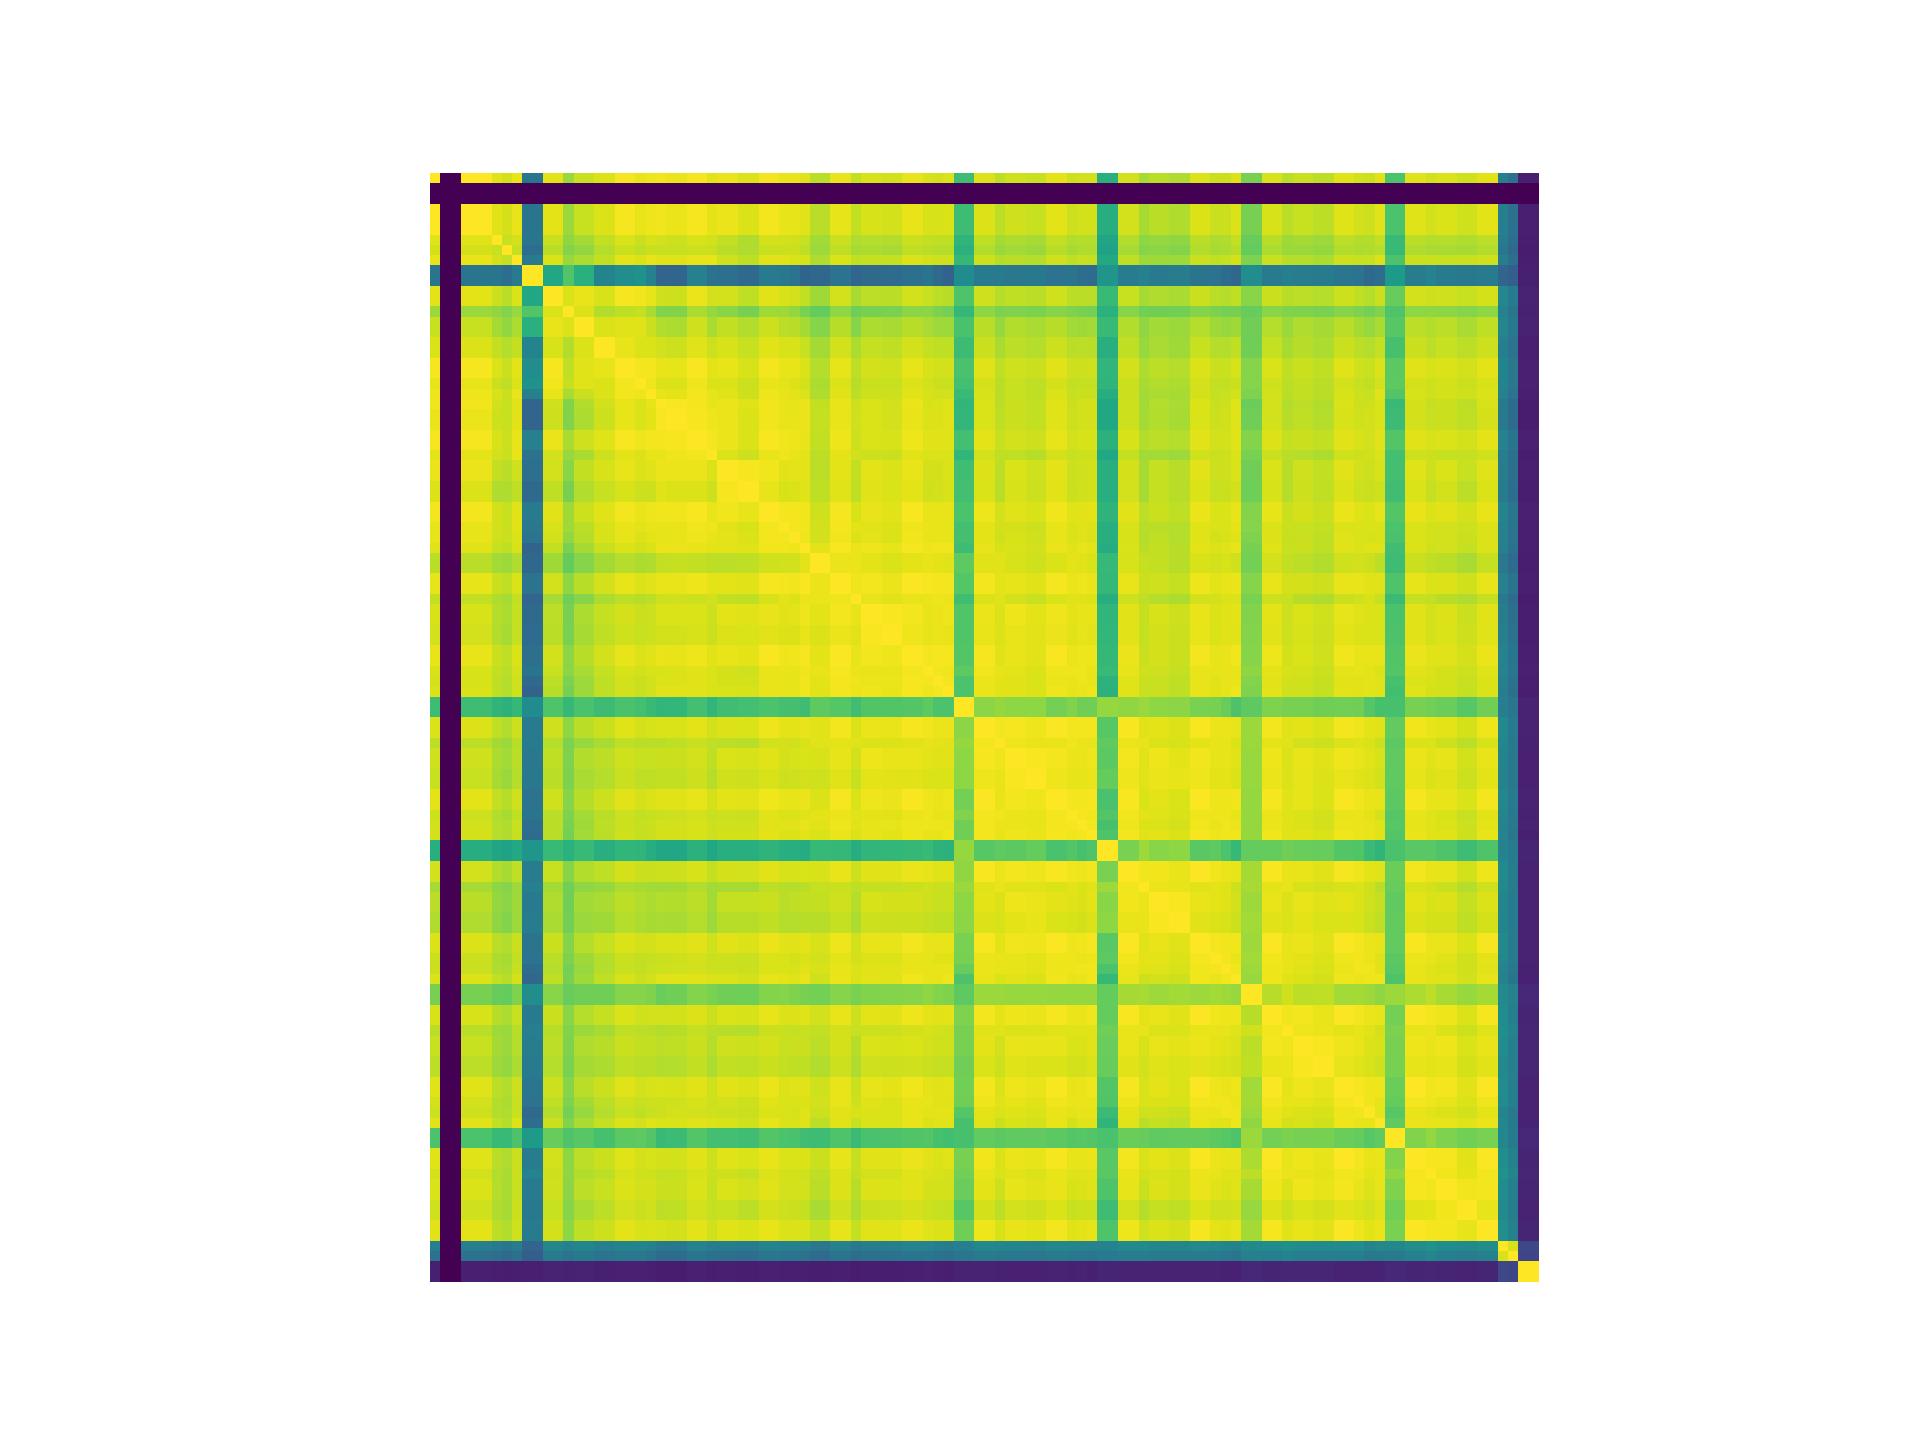
\includegraphics[width=0.5\textwidth]{rsa-cka-base-pretrained-frozen.png}
    \end{figure}
\end{frame}
\begin{frame}{Base Model}{RSA of Frozen Pretrained and Non-Pretrained Models}
    \begin{figure}
        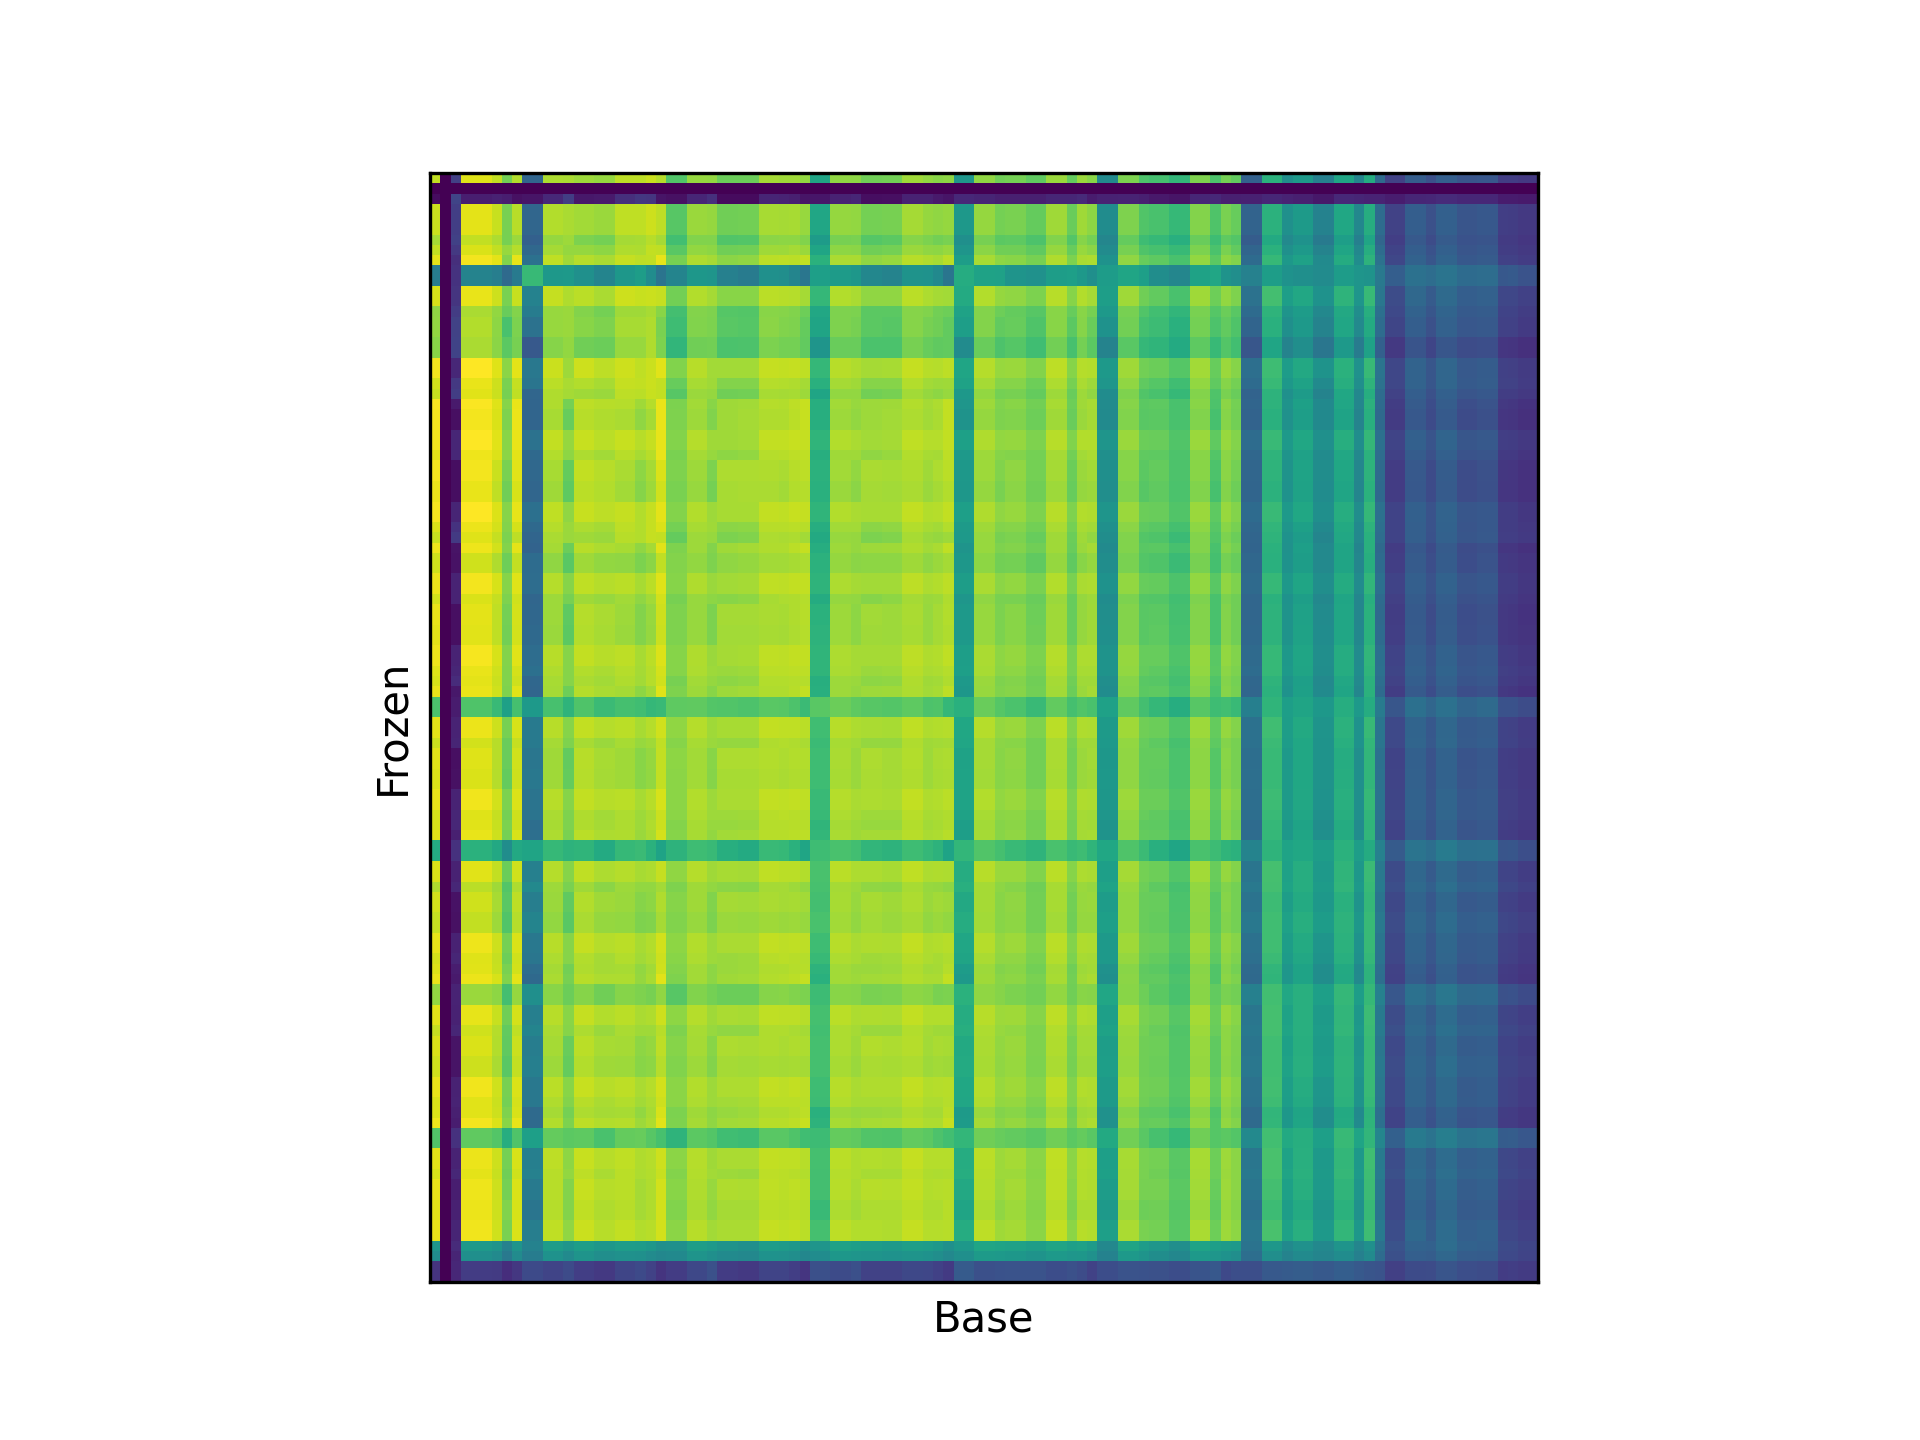
\includegraphics[width=0.5\textwidth]{rsa-cka-base-frozen-scratch.png}
    \end{figure}
\end{frame}

\begin{frame}{Obfuscated Benign Model}{Accuracy}
    \begin{figure}
        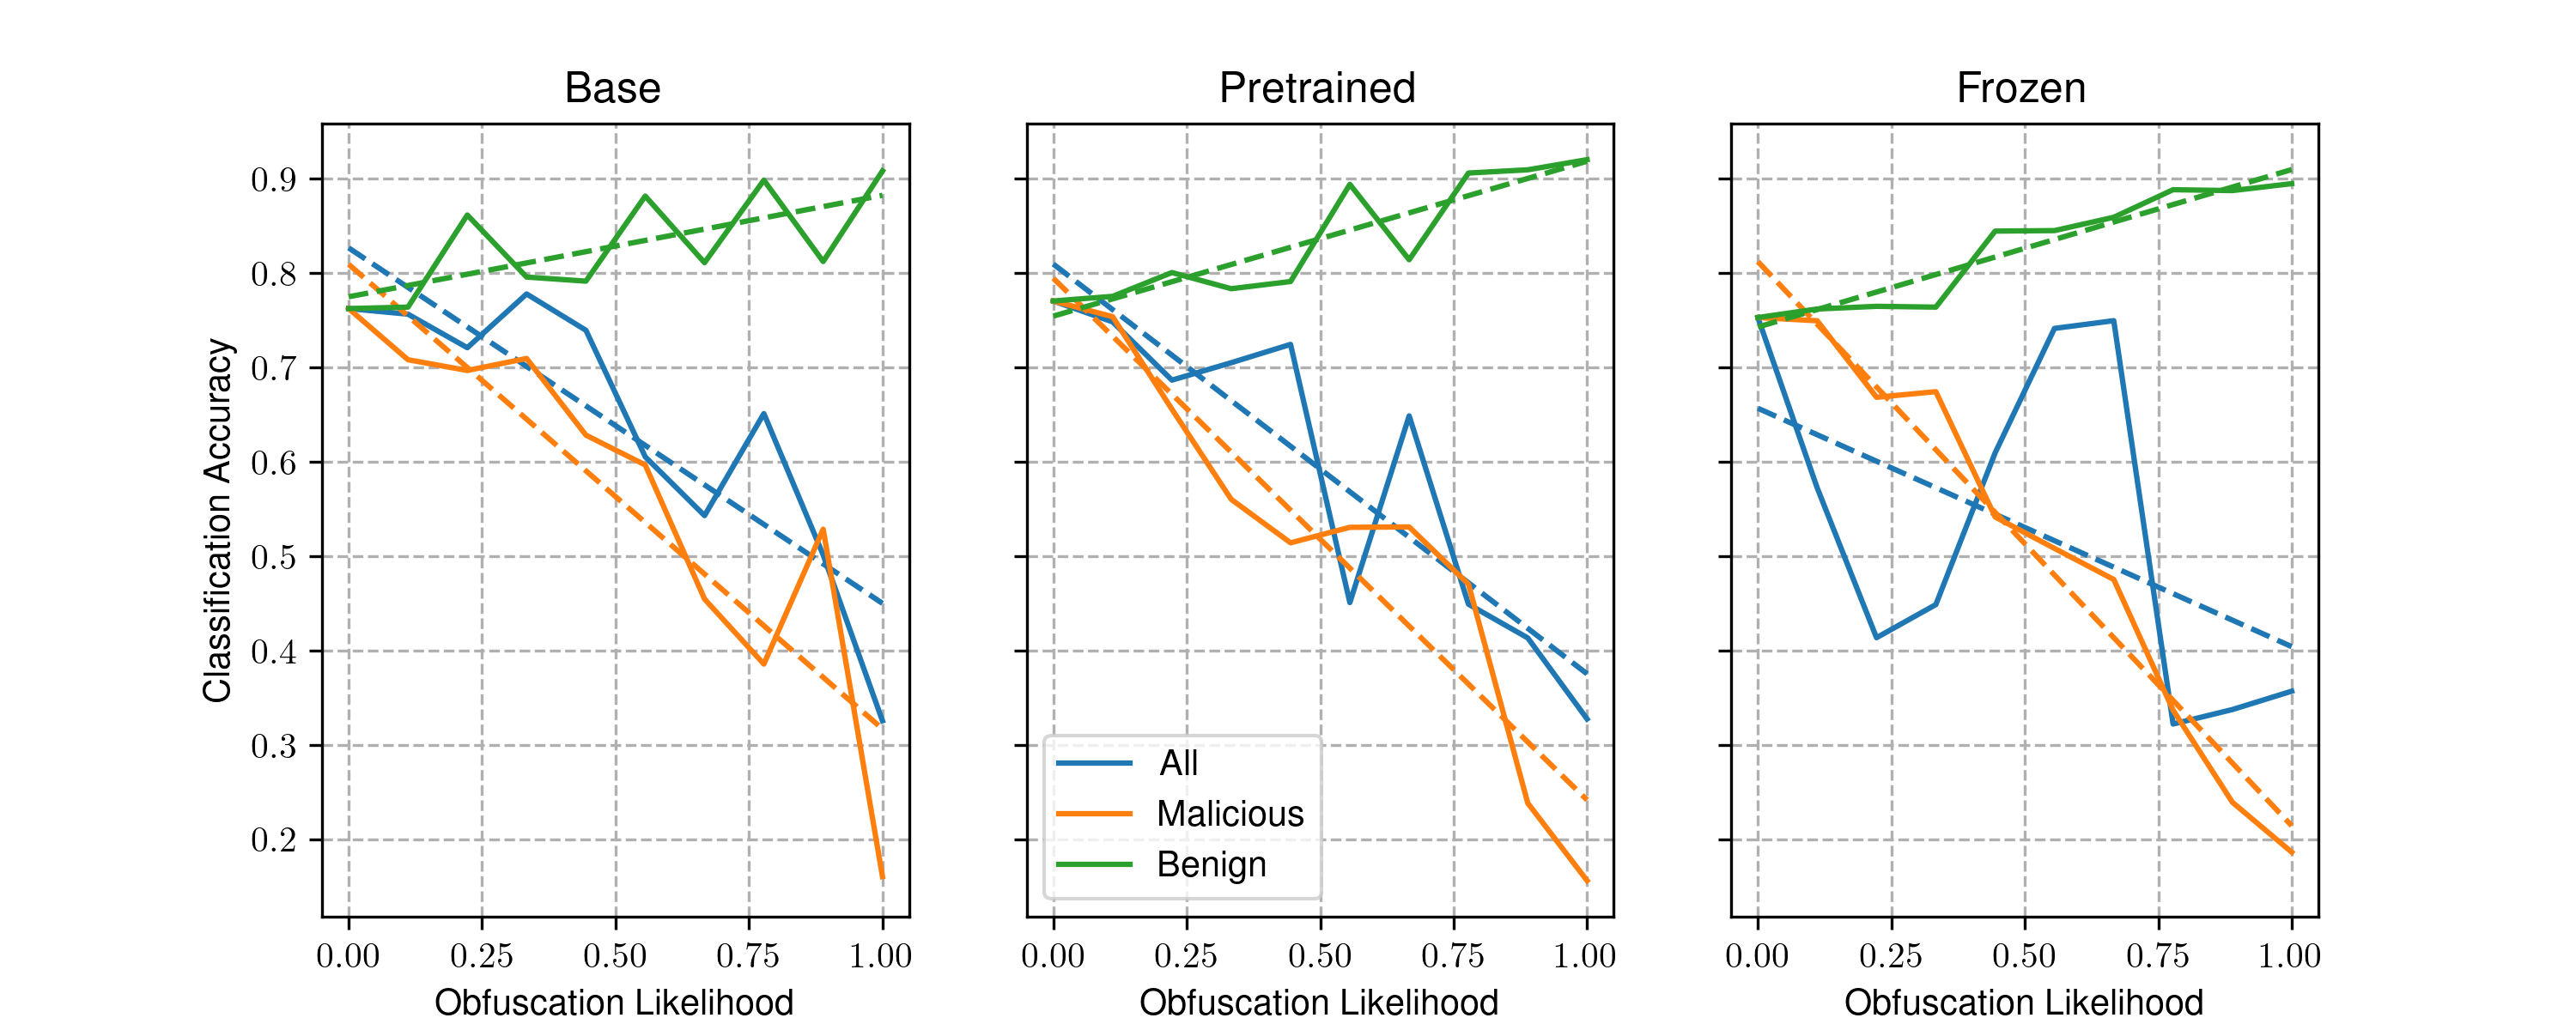
\includegraphics[width=\textwidth]{seq-obf-seq-level-ob.png}
        \caption{File-level performance}
    \end{figure} 
\end{frame}

\begin{frame}{Obfuscated Benign Model}{F1 Score}
    \begin{figure}
        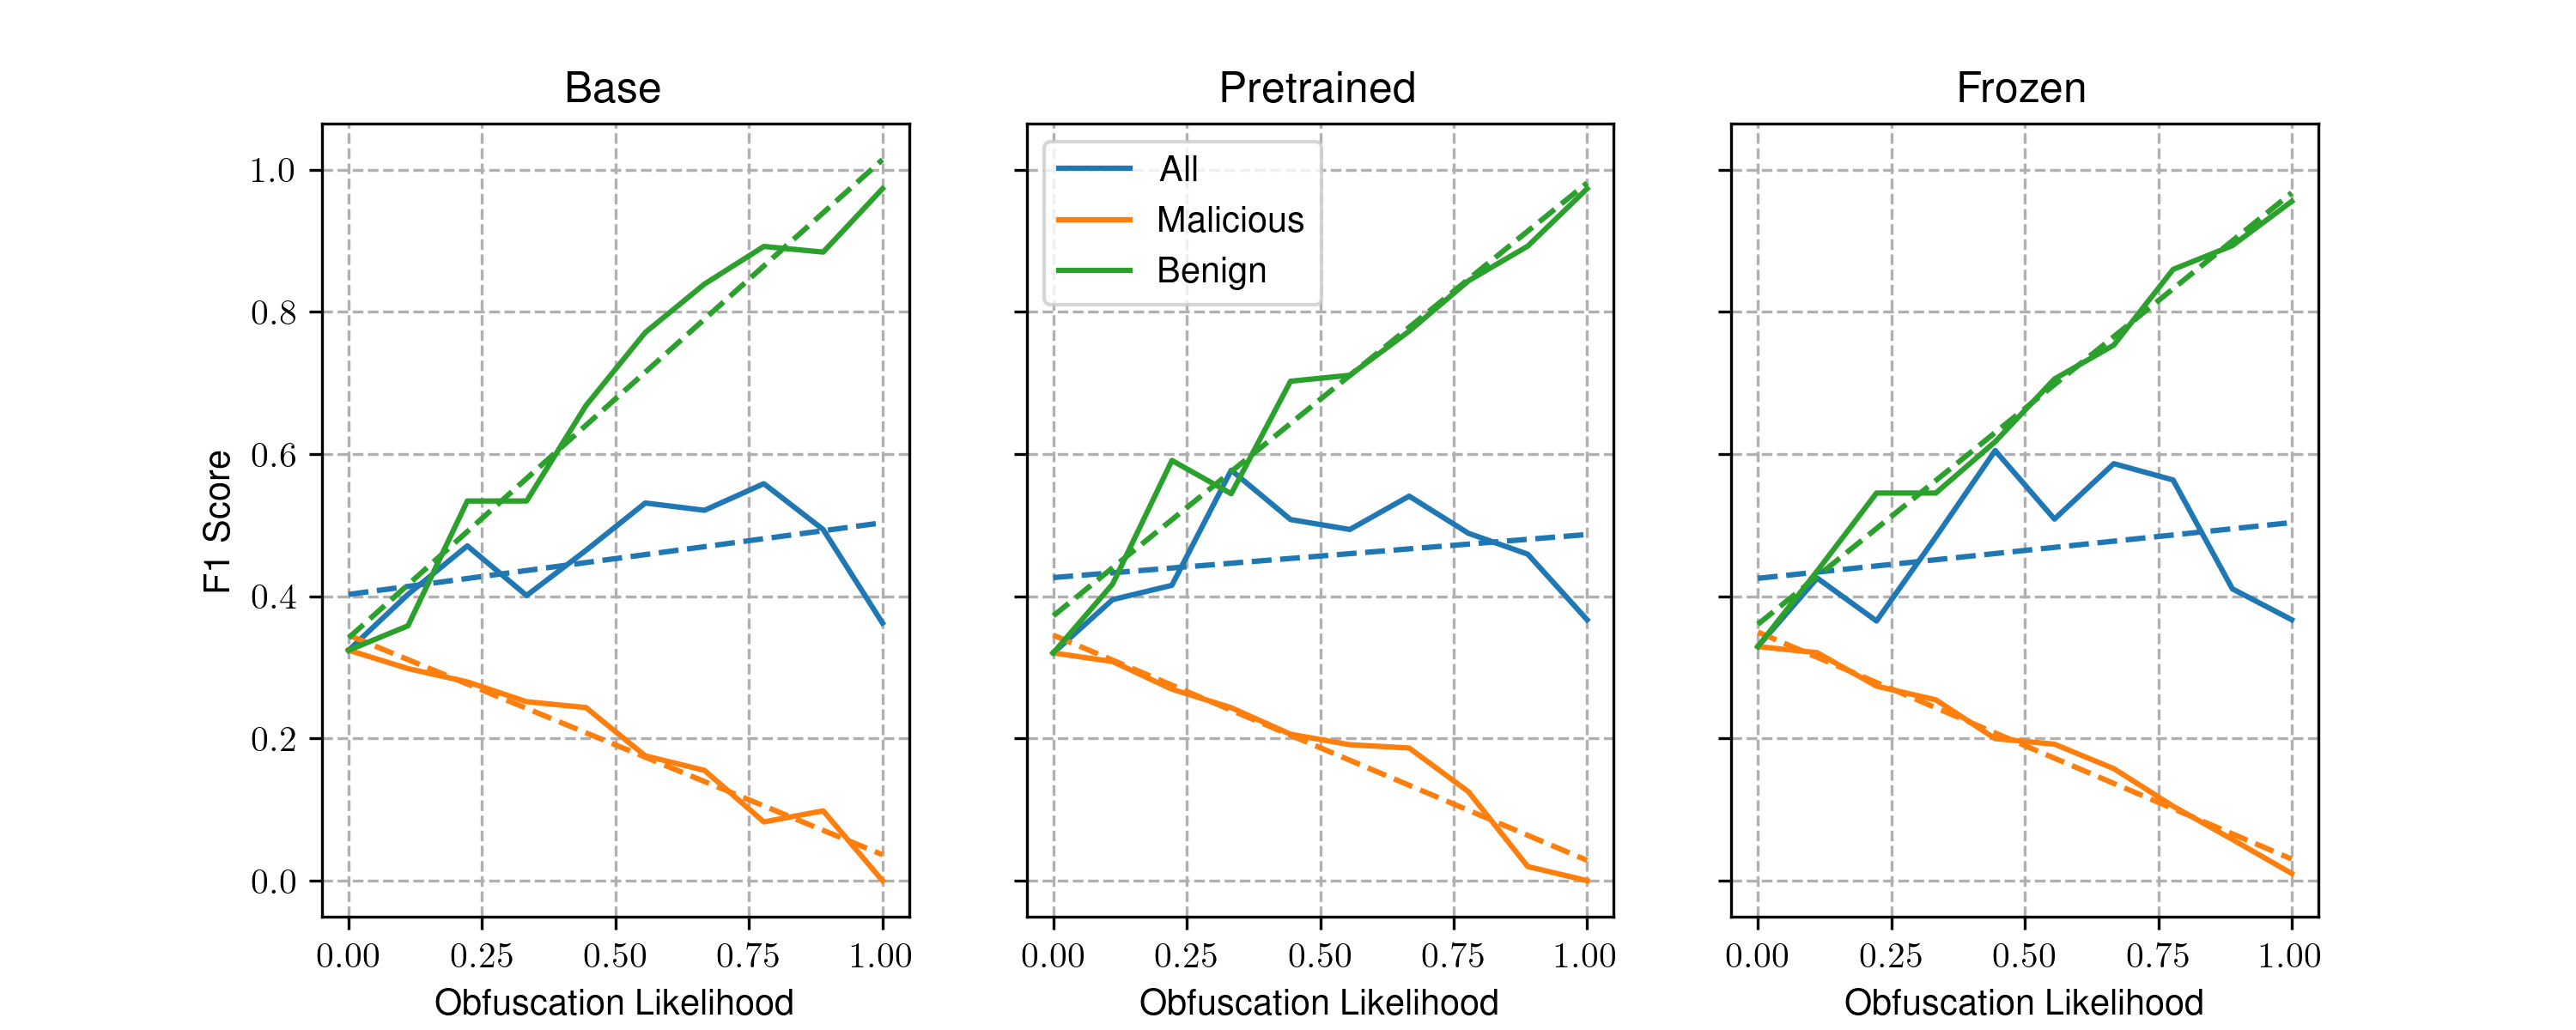
\includegraphics[width=\textwidth]{seq-obf-file-level-ob-f1-score.png}
        \caption{File Level F1 score}
    \end{figure} 
\end{frame}
\begin{frame}{Obfuscated Benign Model}{Sequence Accuracy}
    \begin{figure}
        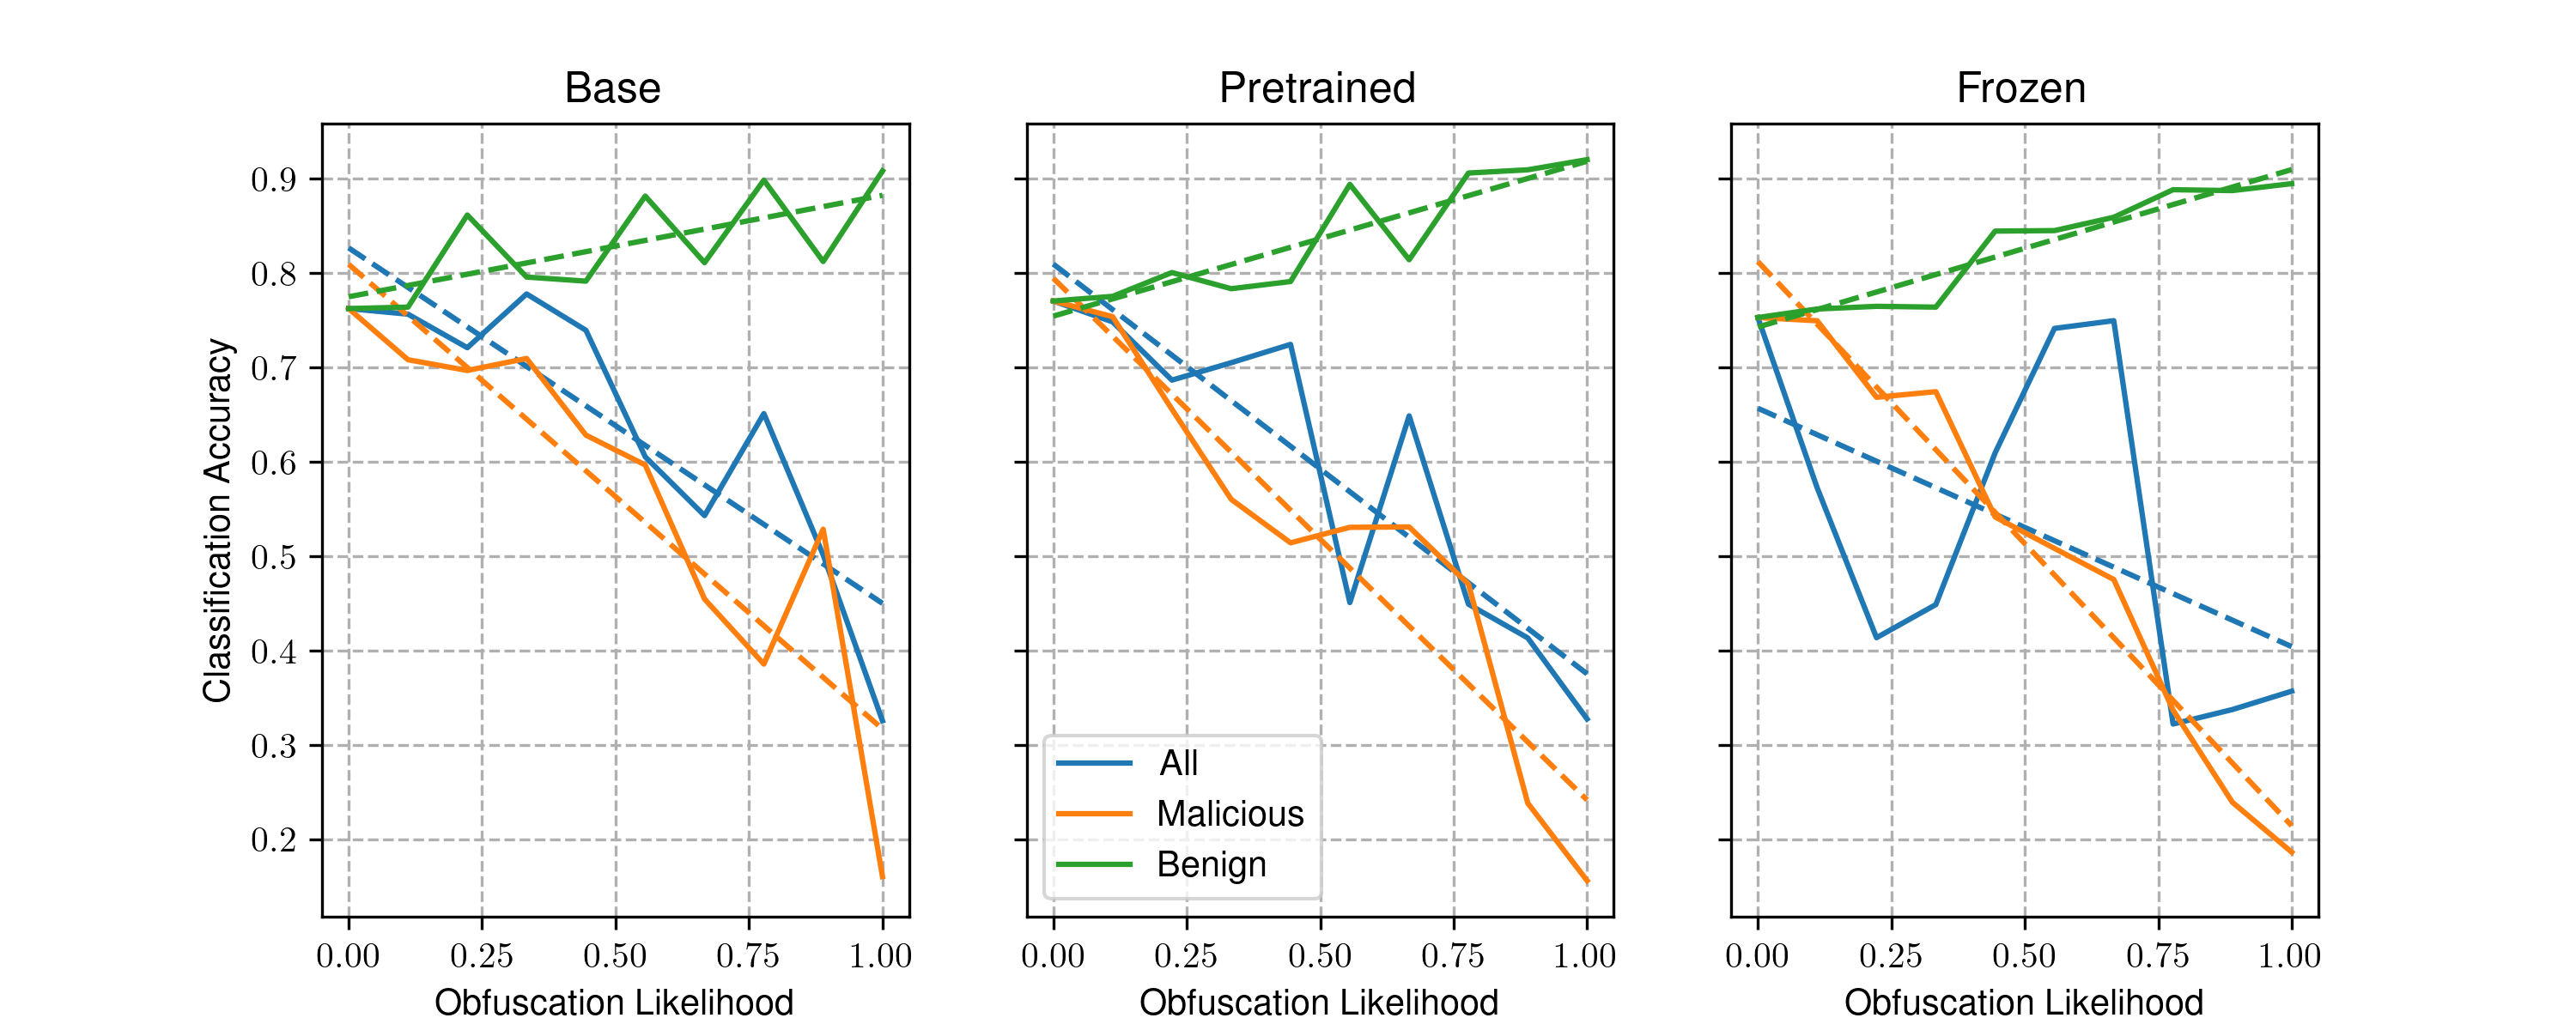
\includegraphics[width=\textwidth]{seq-obf-seq-level-ob.png}
        \caption{Sequence-level performance}
    \end{figure} 
\end{frame}

\begin{frame}{Obfuscated Benign Model}{Certainty}
    \begin{figure}
        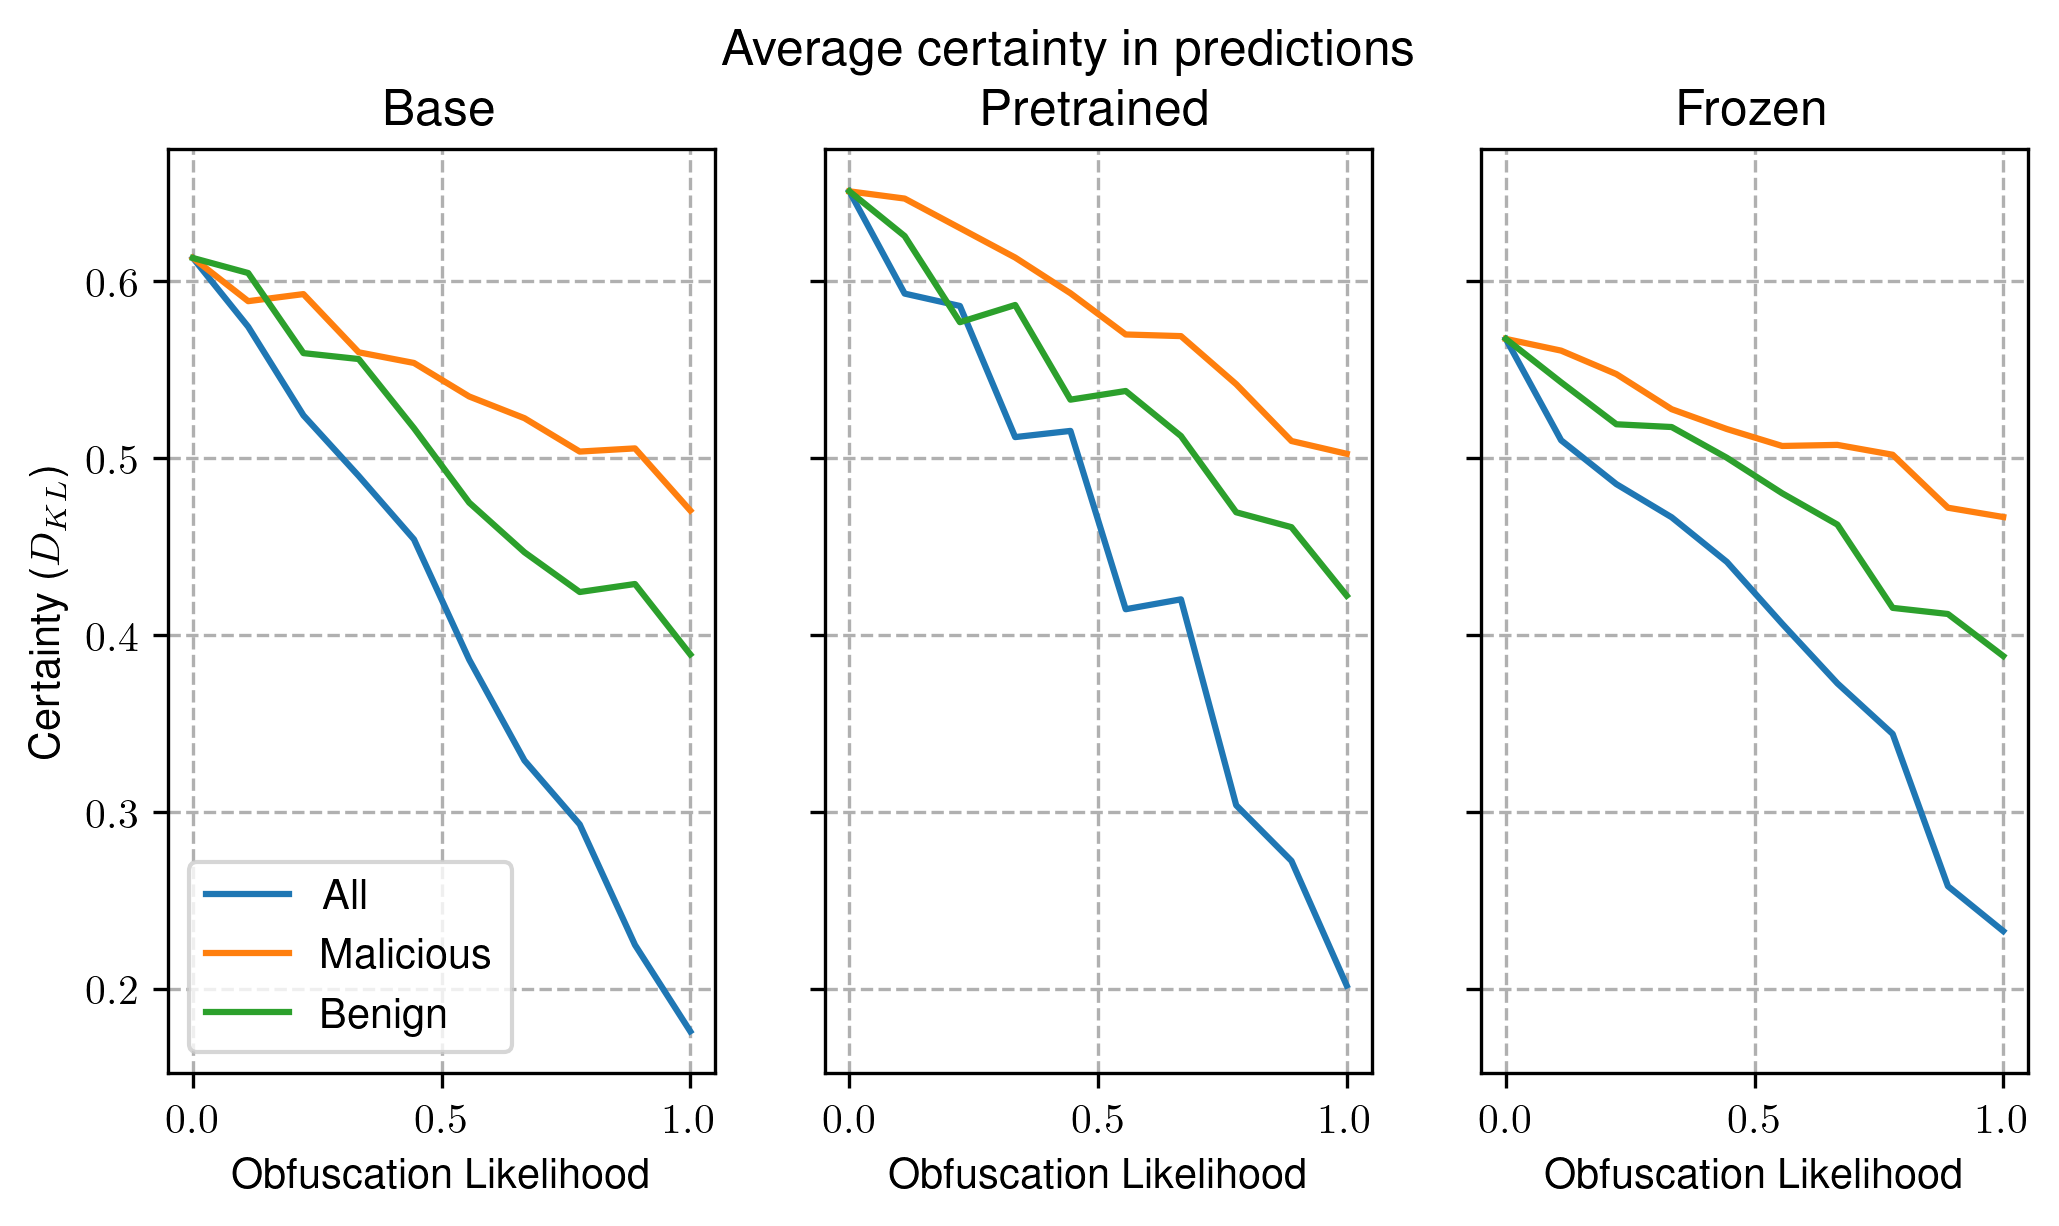
\includegraphics[width=\textwidth]{seq-obf-certainty-ob.png}
        \caption{Confidence}
    \end{figure} 
\end{frame}

\begin{frame}{Obfuscated Benign Model}{RSA of Pretrained and Non-Pretrained Models}
    \begin{figure}
        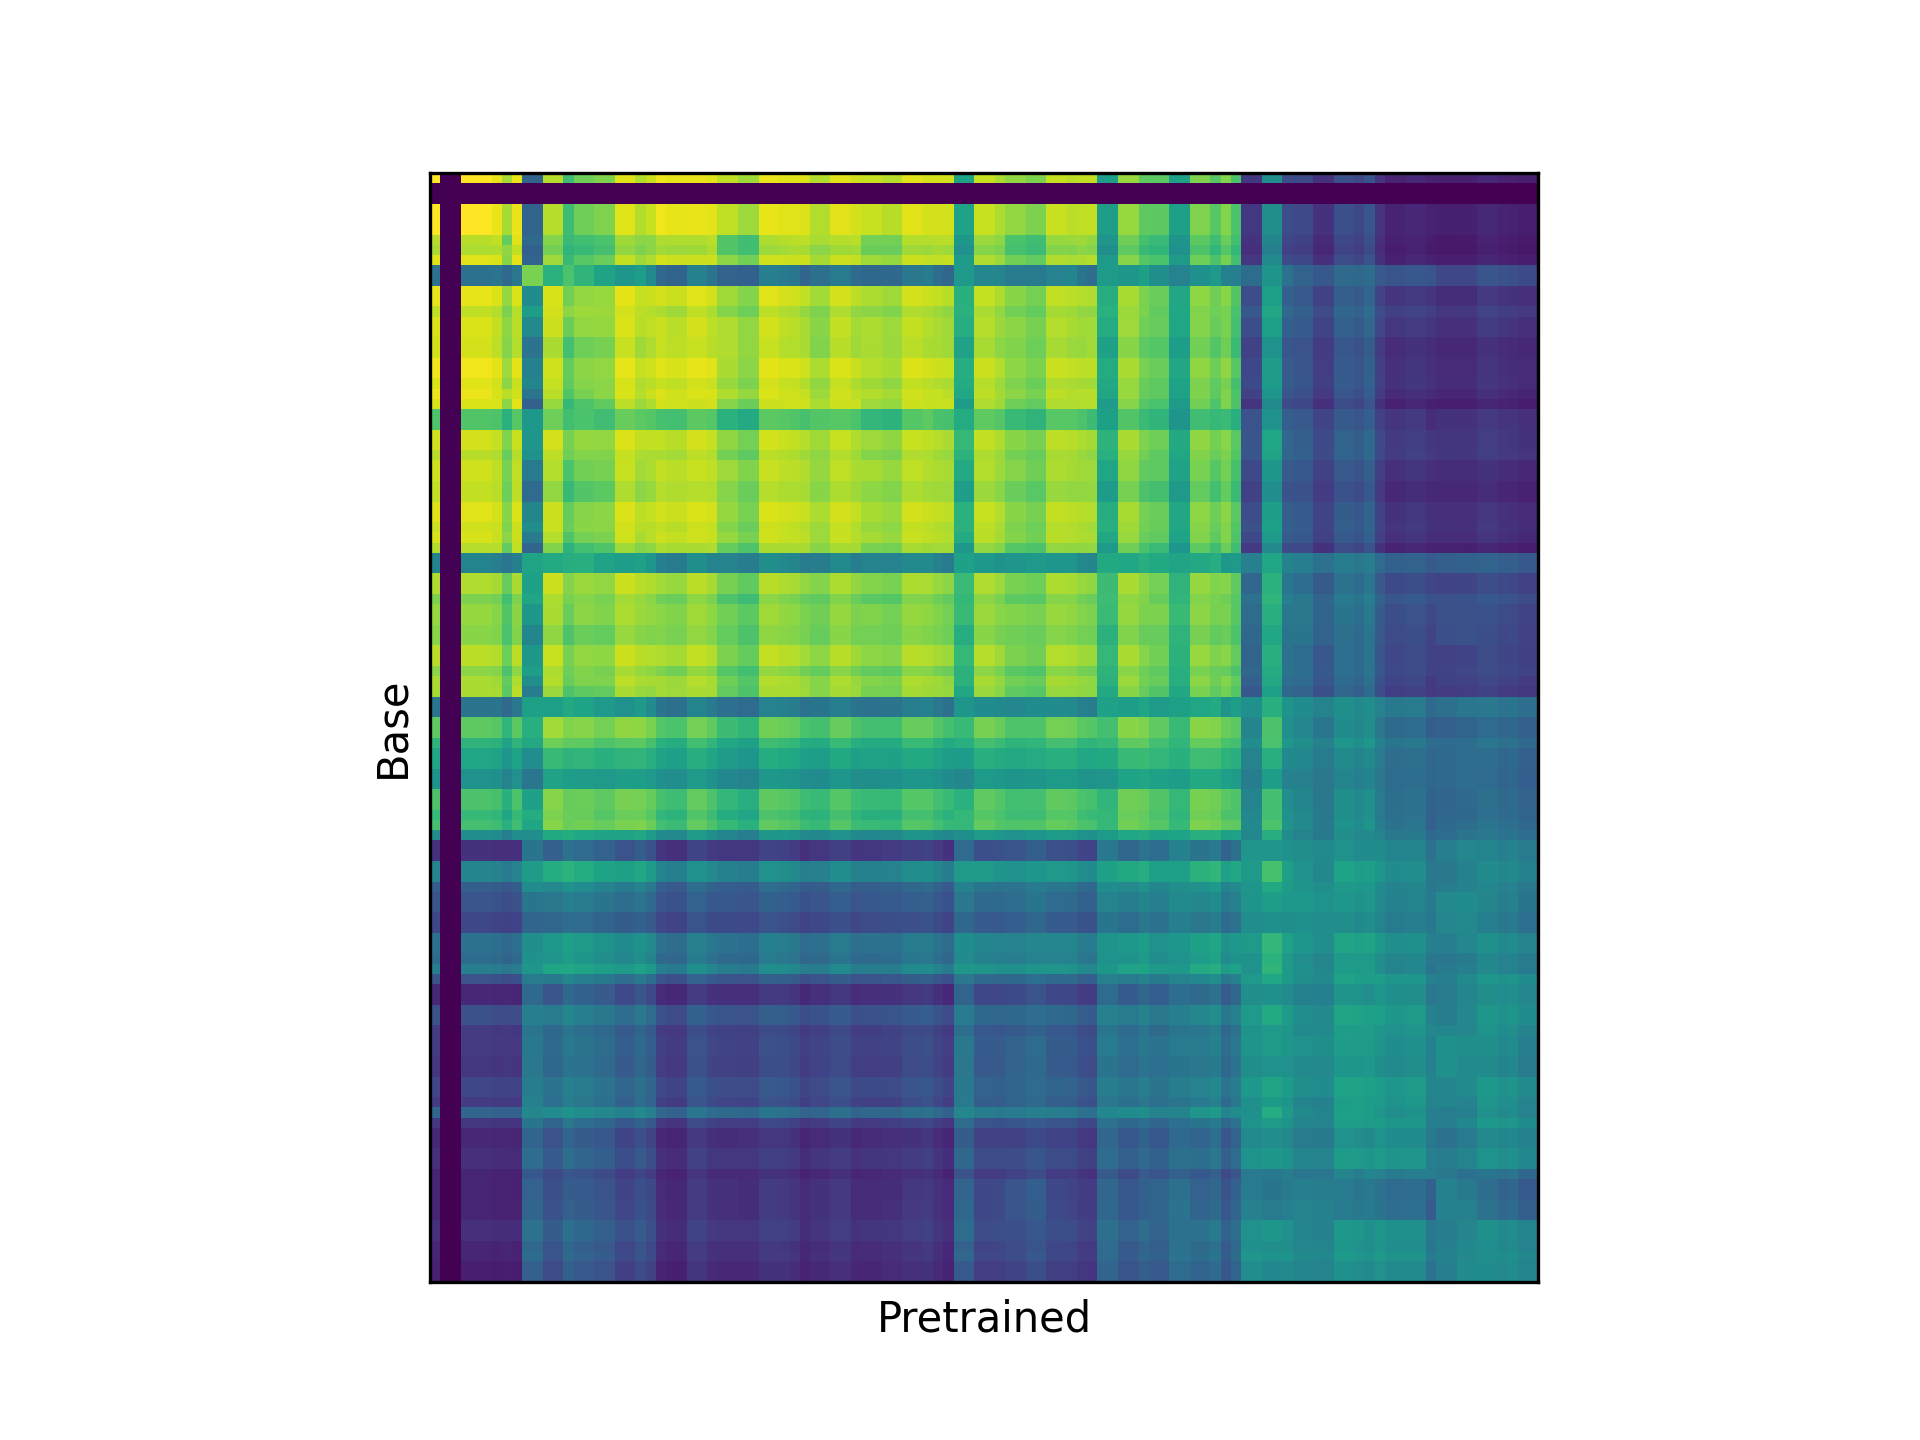
\includegraphics[width=0.5\textwidth]{rsa-cka-ob-pretrained-scratch.png}
    \end{figure}
\end{frame}

\begin{frame}{Obfuscated Benign Model}{RSA of Pretrained and Frozen Pretrained Models}
    \begin{figure}
        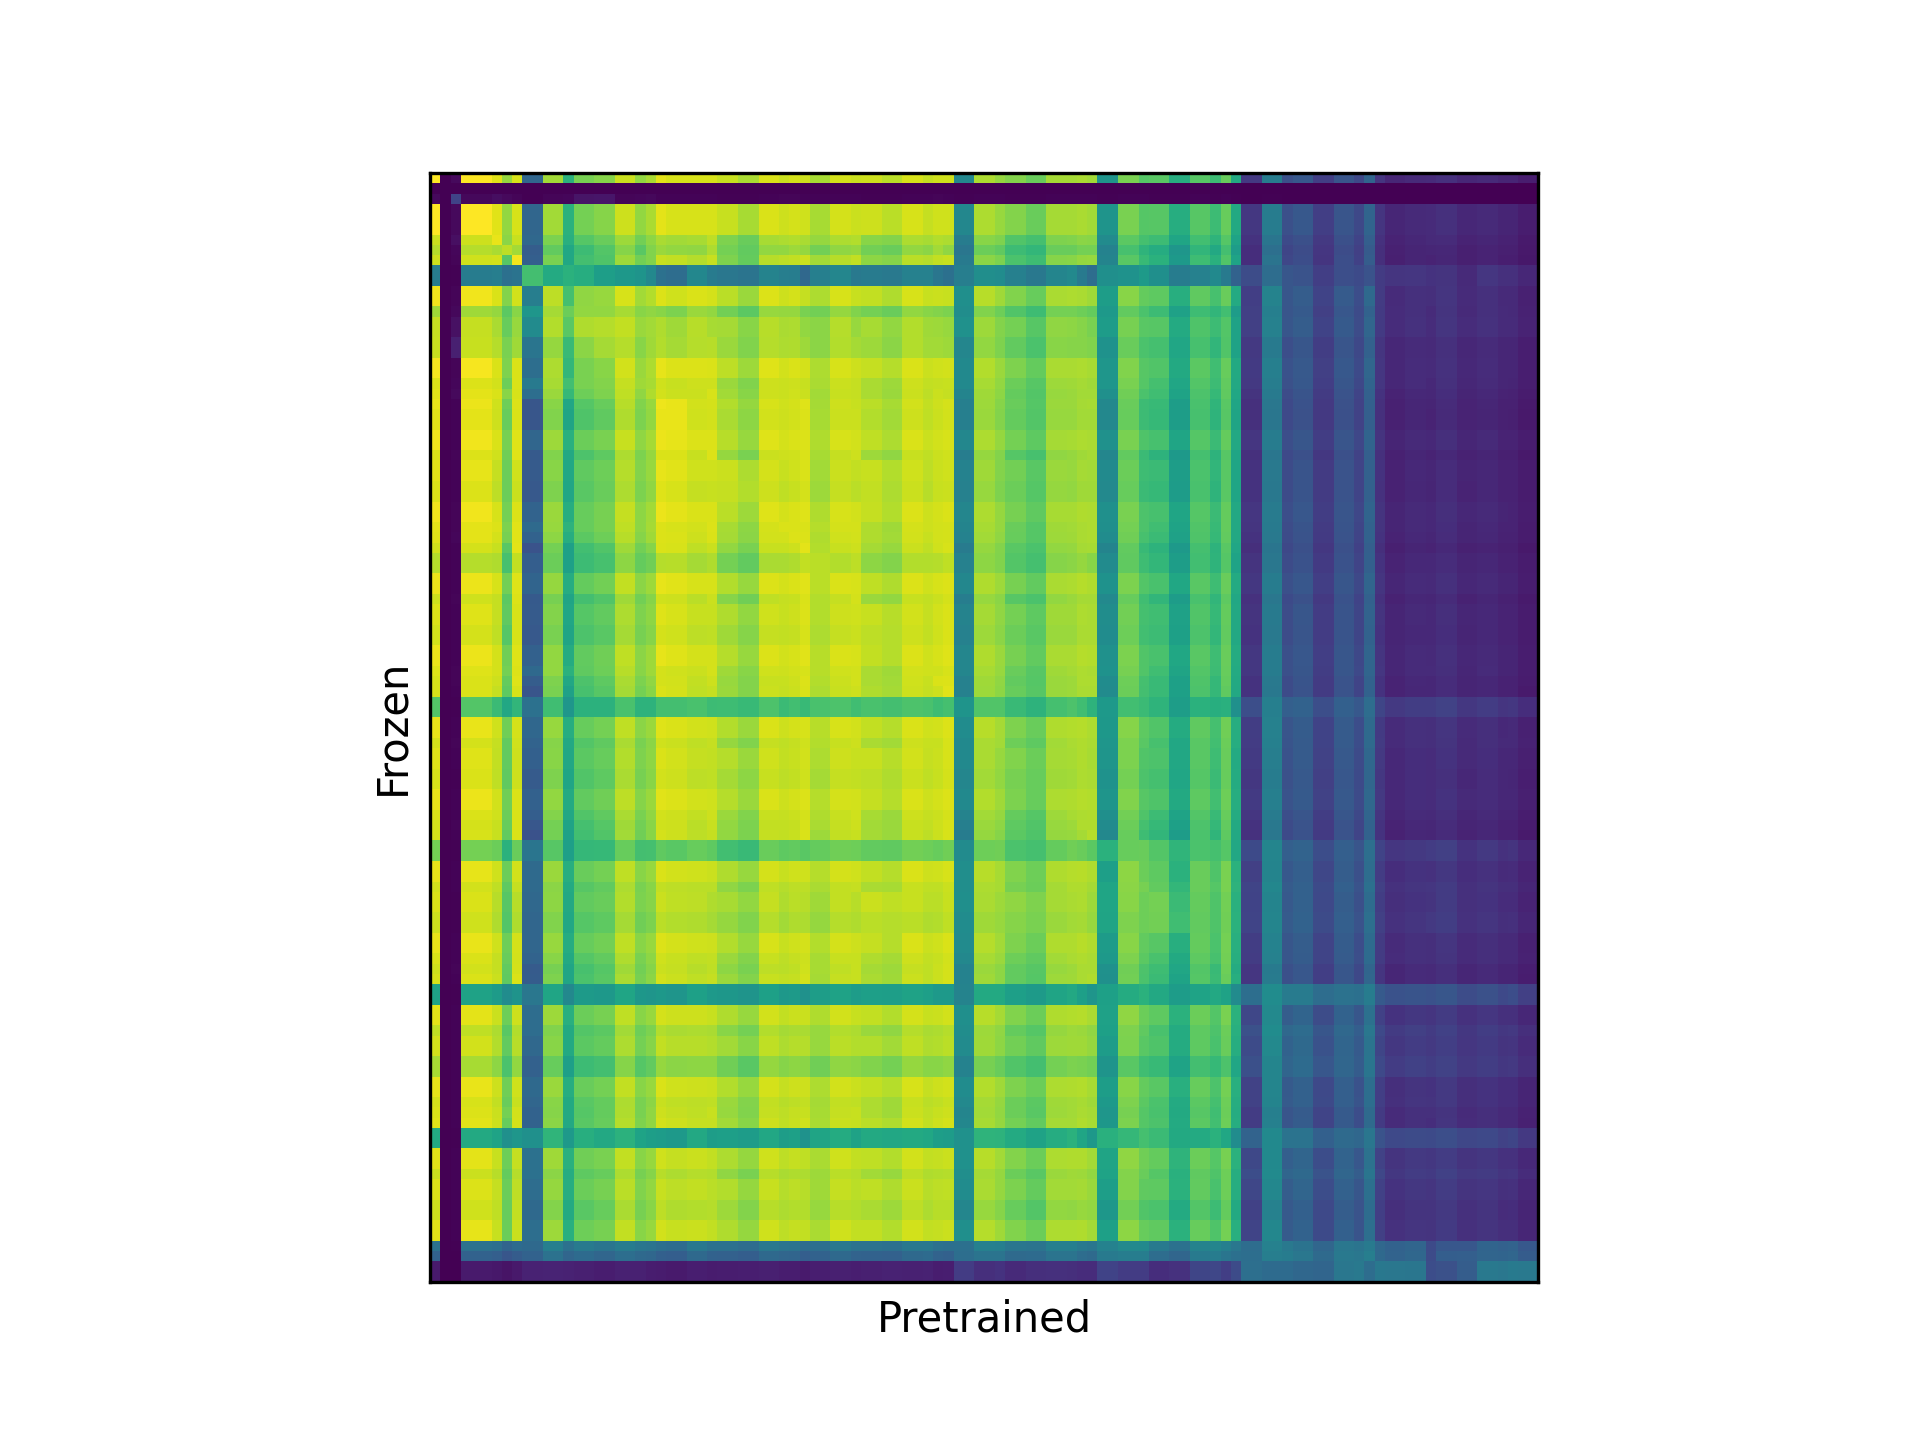
\includegraphics[width=0.5\textwidth]{rsa-cka-ob-pretrained-frozen.png}
    \end{figure}
\end{frame}
\begin{frame}{Obfuscated Benign Model}{RSA of Frozen Pretrained and Non-Pretrained Models}
    \begin{figure}
        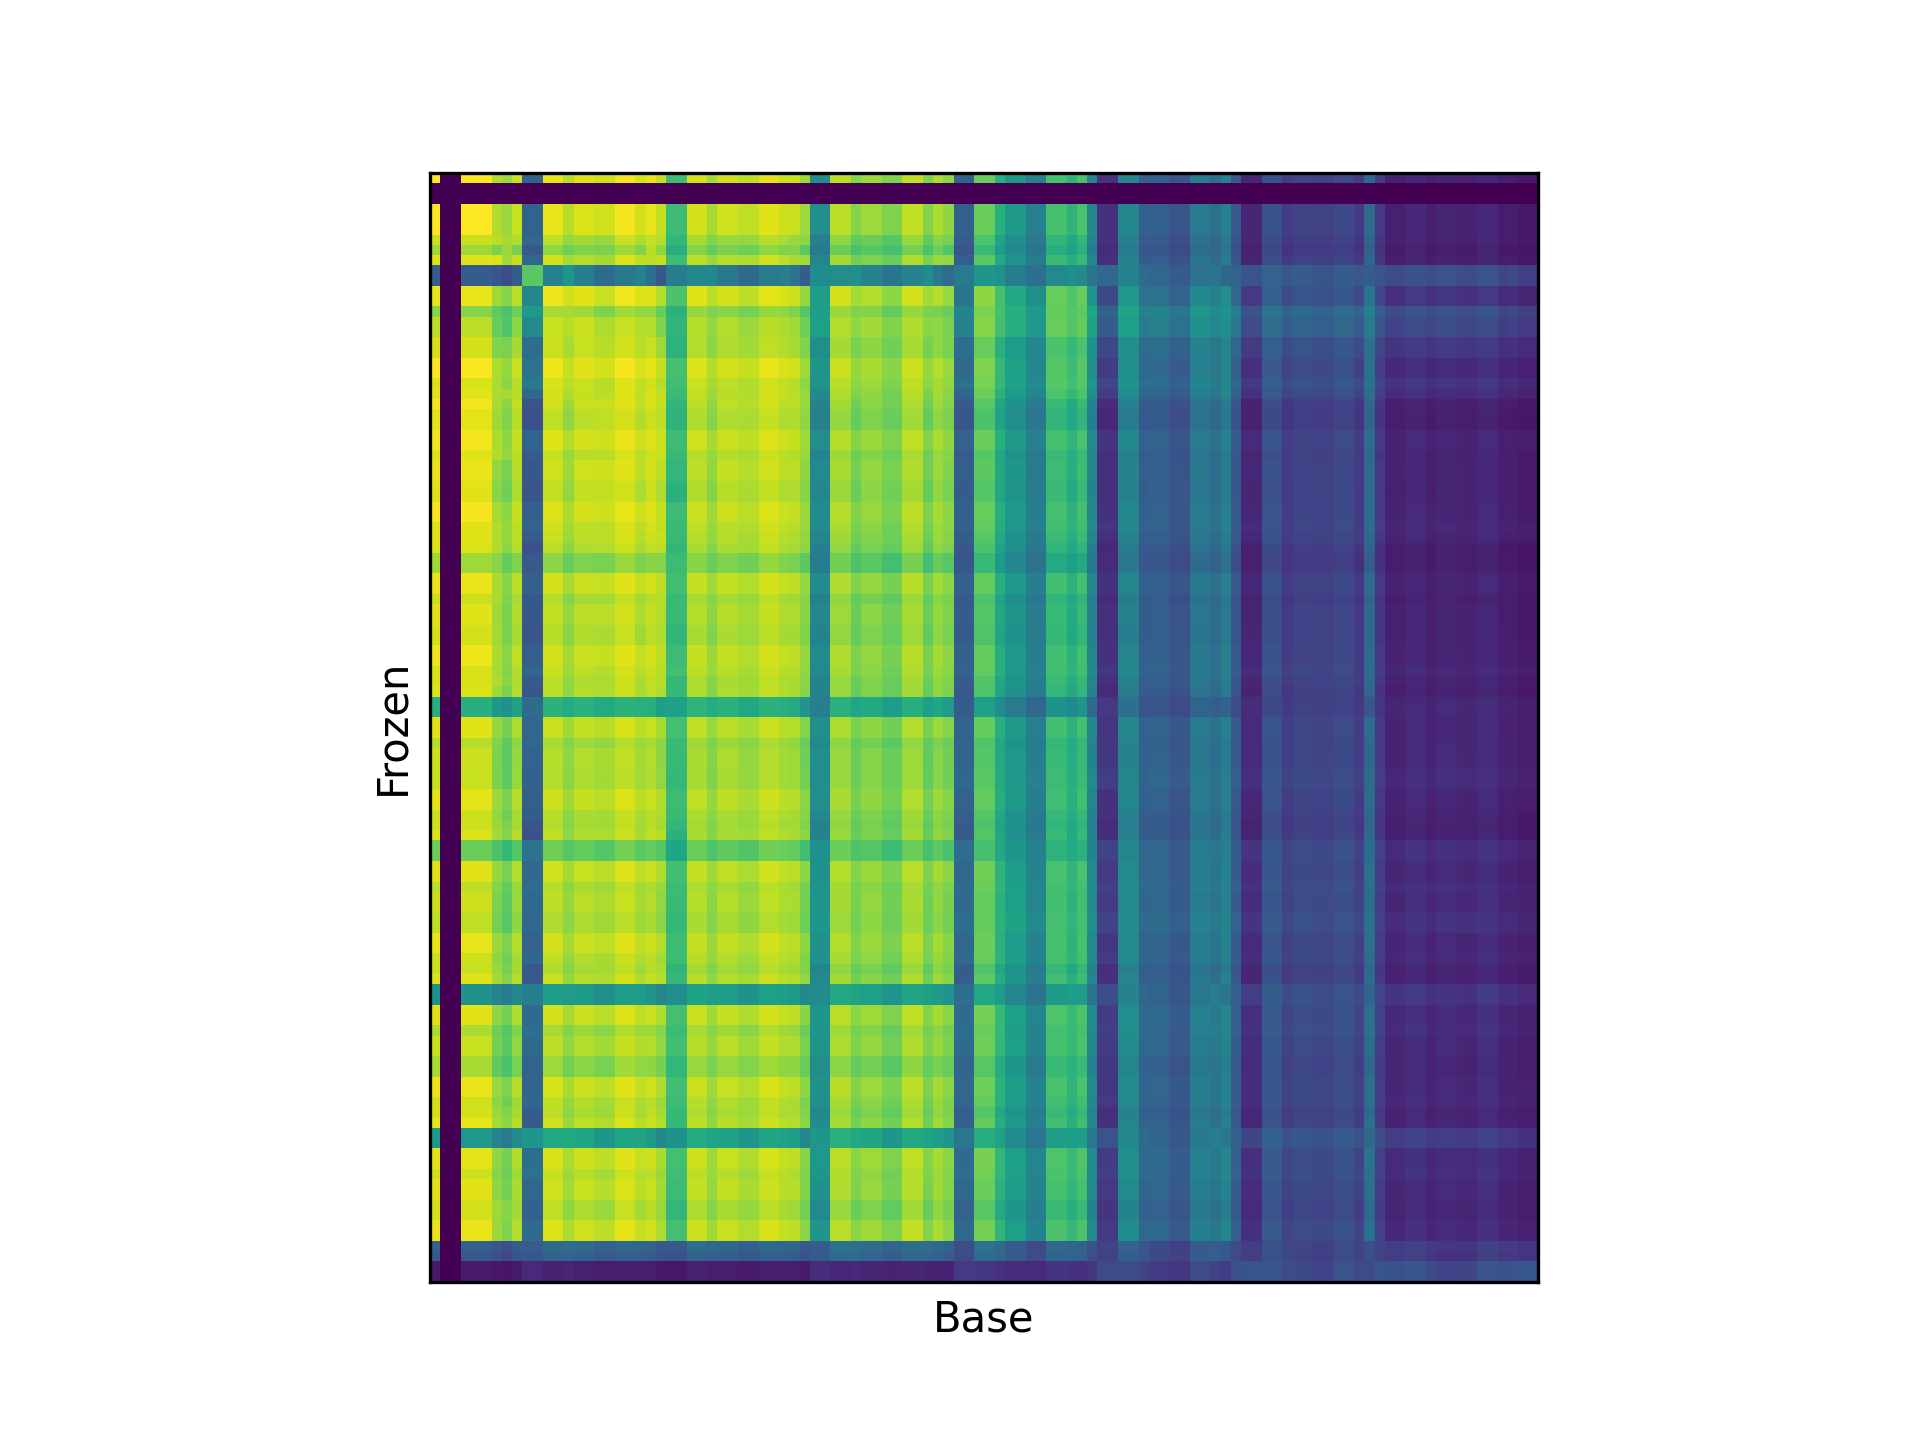
\includegraphics[width=0.5\textwidth]{rsa-cka-ob-frozen-scratch.png}
    \end{figure}
\end{frame}

\begin{frame}{Partially Obfuscated Benign Model}{Accuracy}
    \begin{figure}
        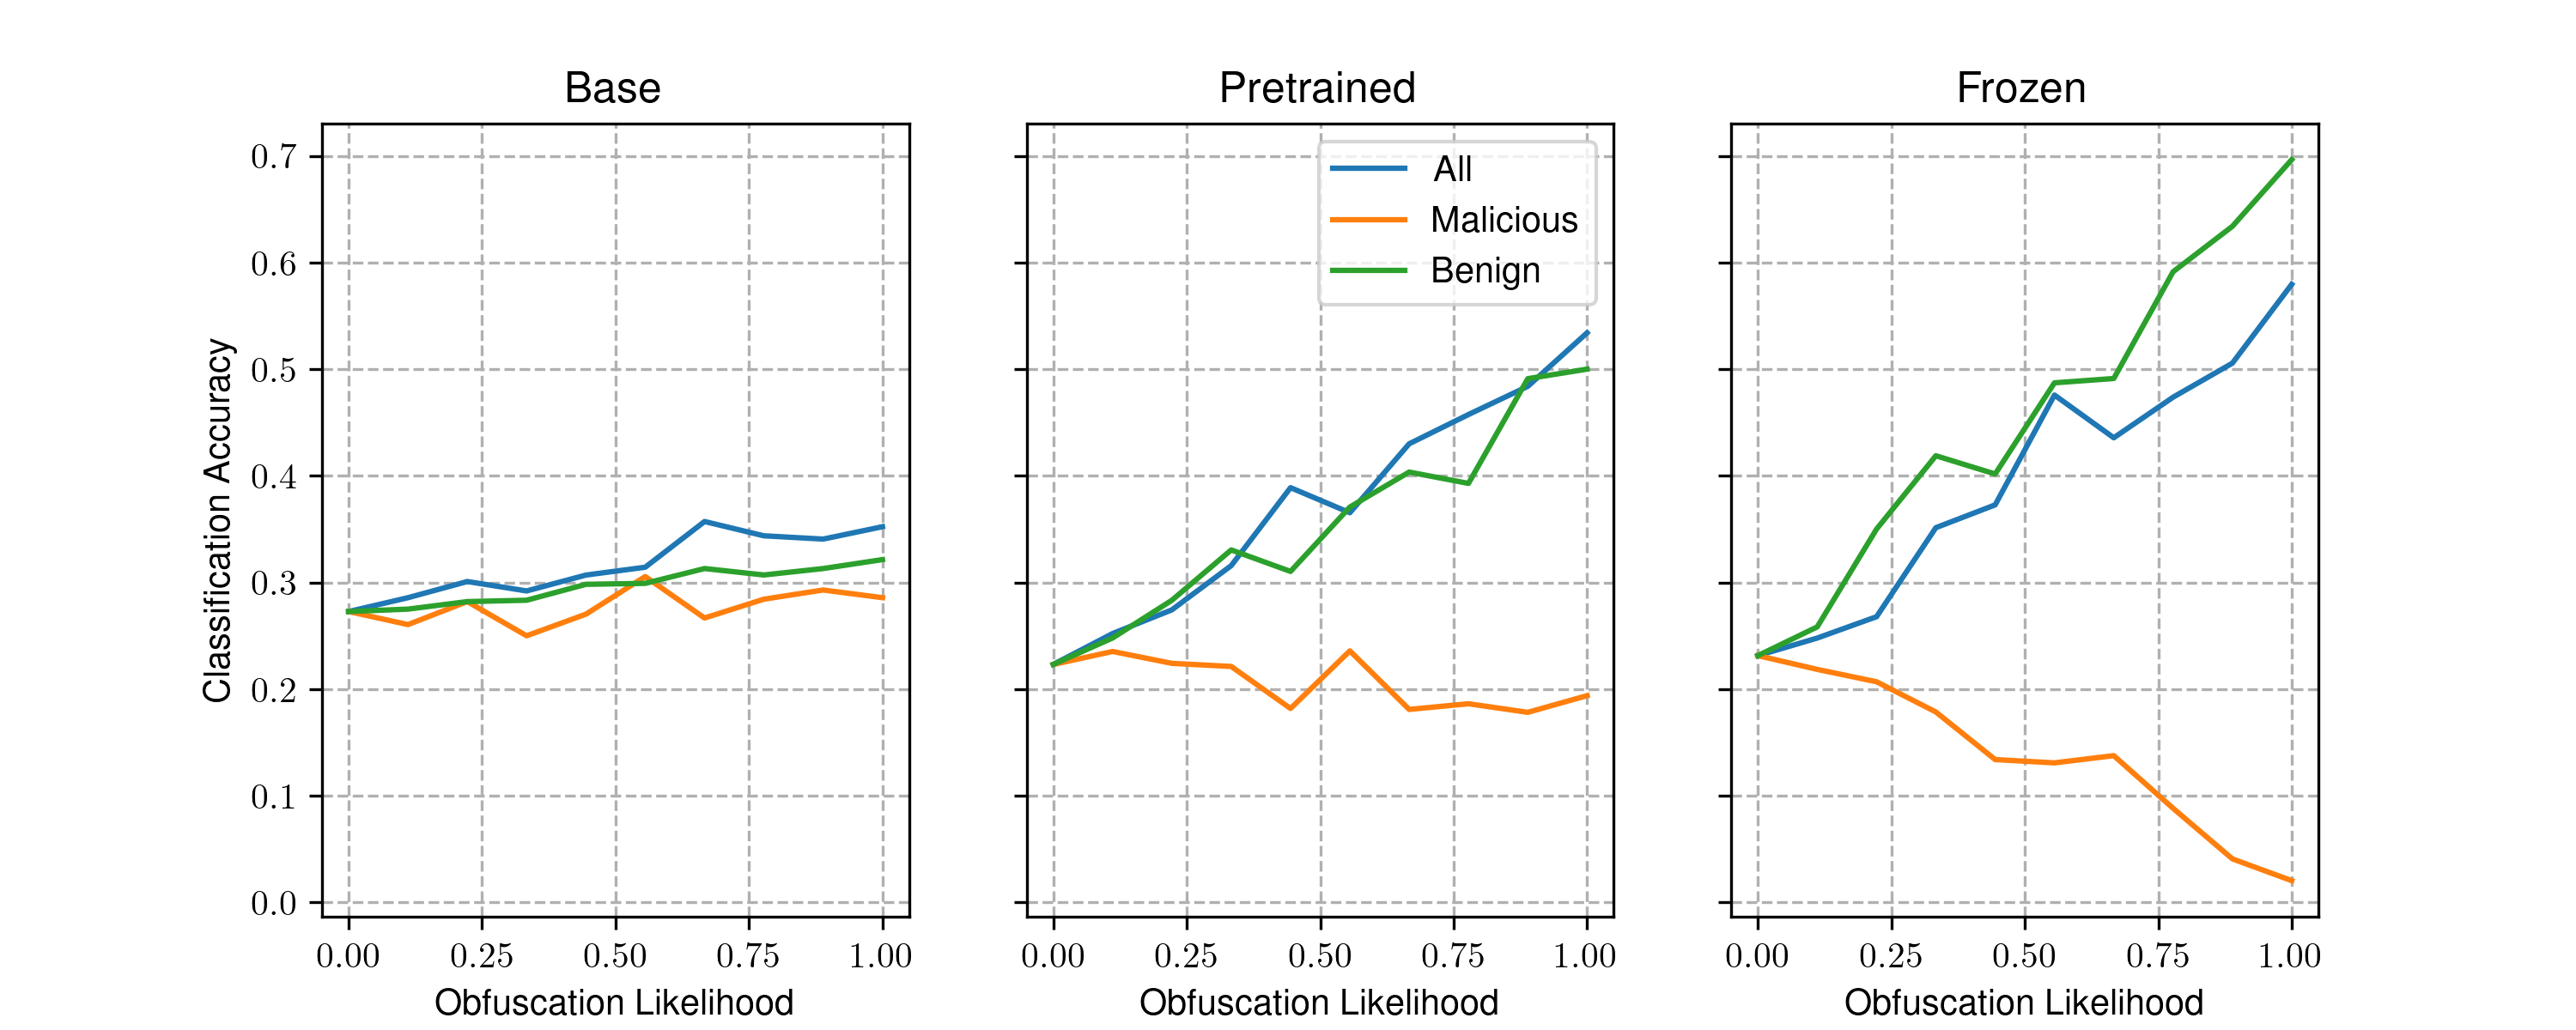
\includegraphics[width=\textwidth]{seq-obf-file-level-pob.png}
        \caption{File Level F1 score}
    \end{figure} 
\end{frame}

\begin{frame}{Partially Obfuscated Benign Model}{F1 Score}
    \begin{figure}
        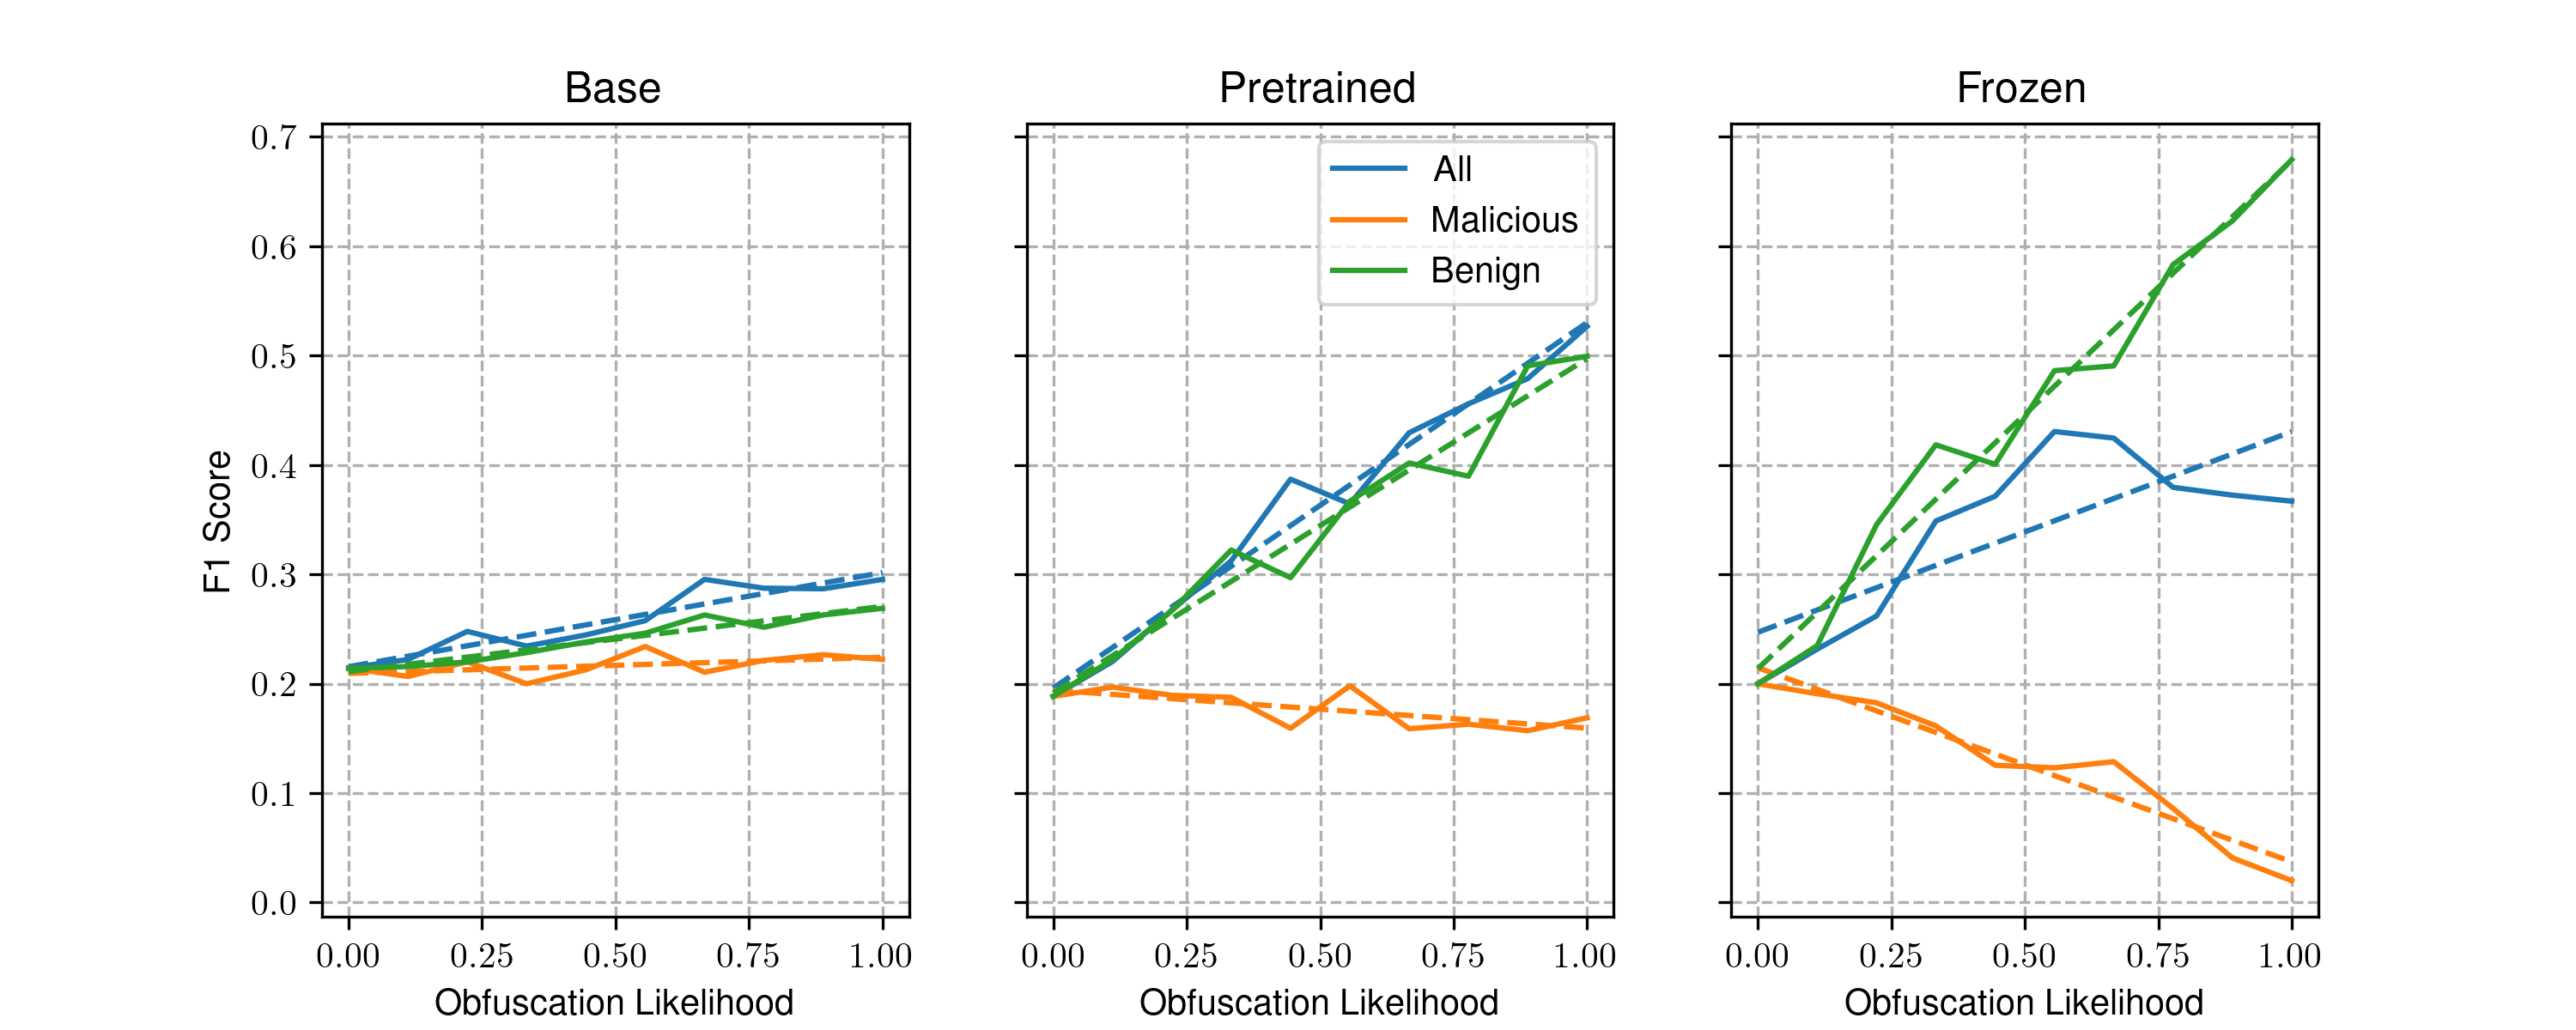
\includegraphics[width=\textwidth]{seq-obf-file-level-pob-f1-score.png}
        \caption{File Level F1 score}
    \end{figure} 
\end{frame}
\begin{frame}{Partially Obfuscated Benign Model}{Sequence Accuracy}
    \begin{figure}
        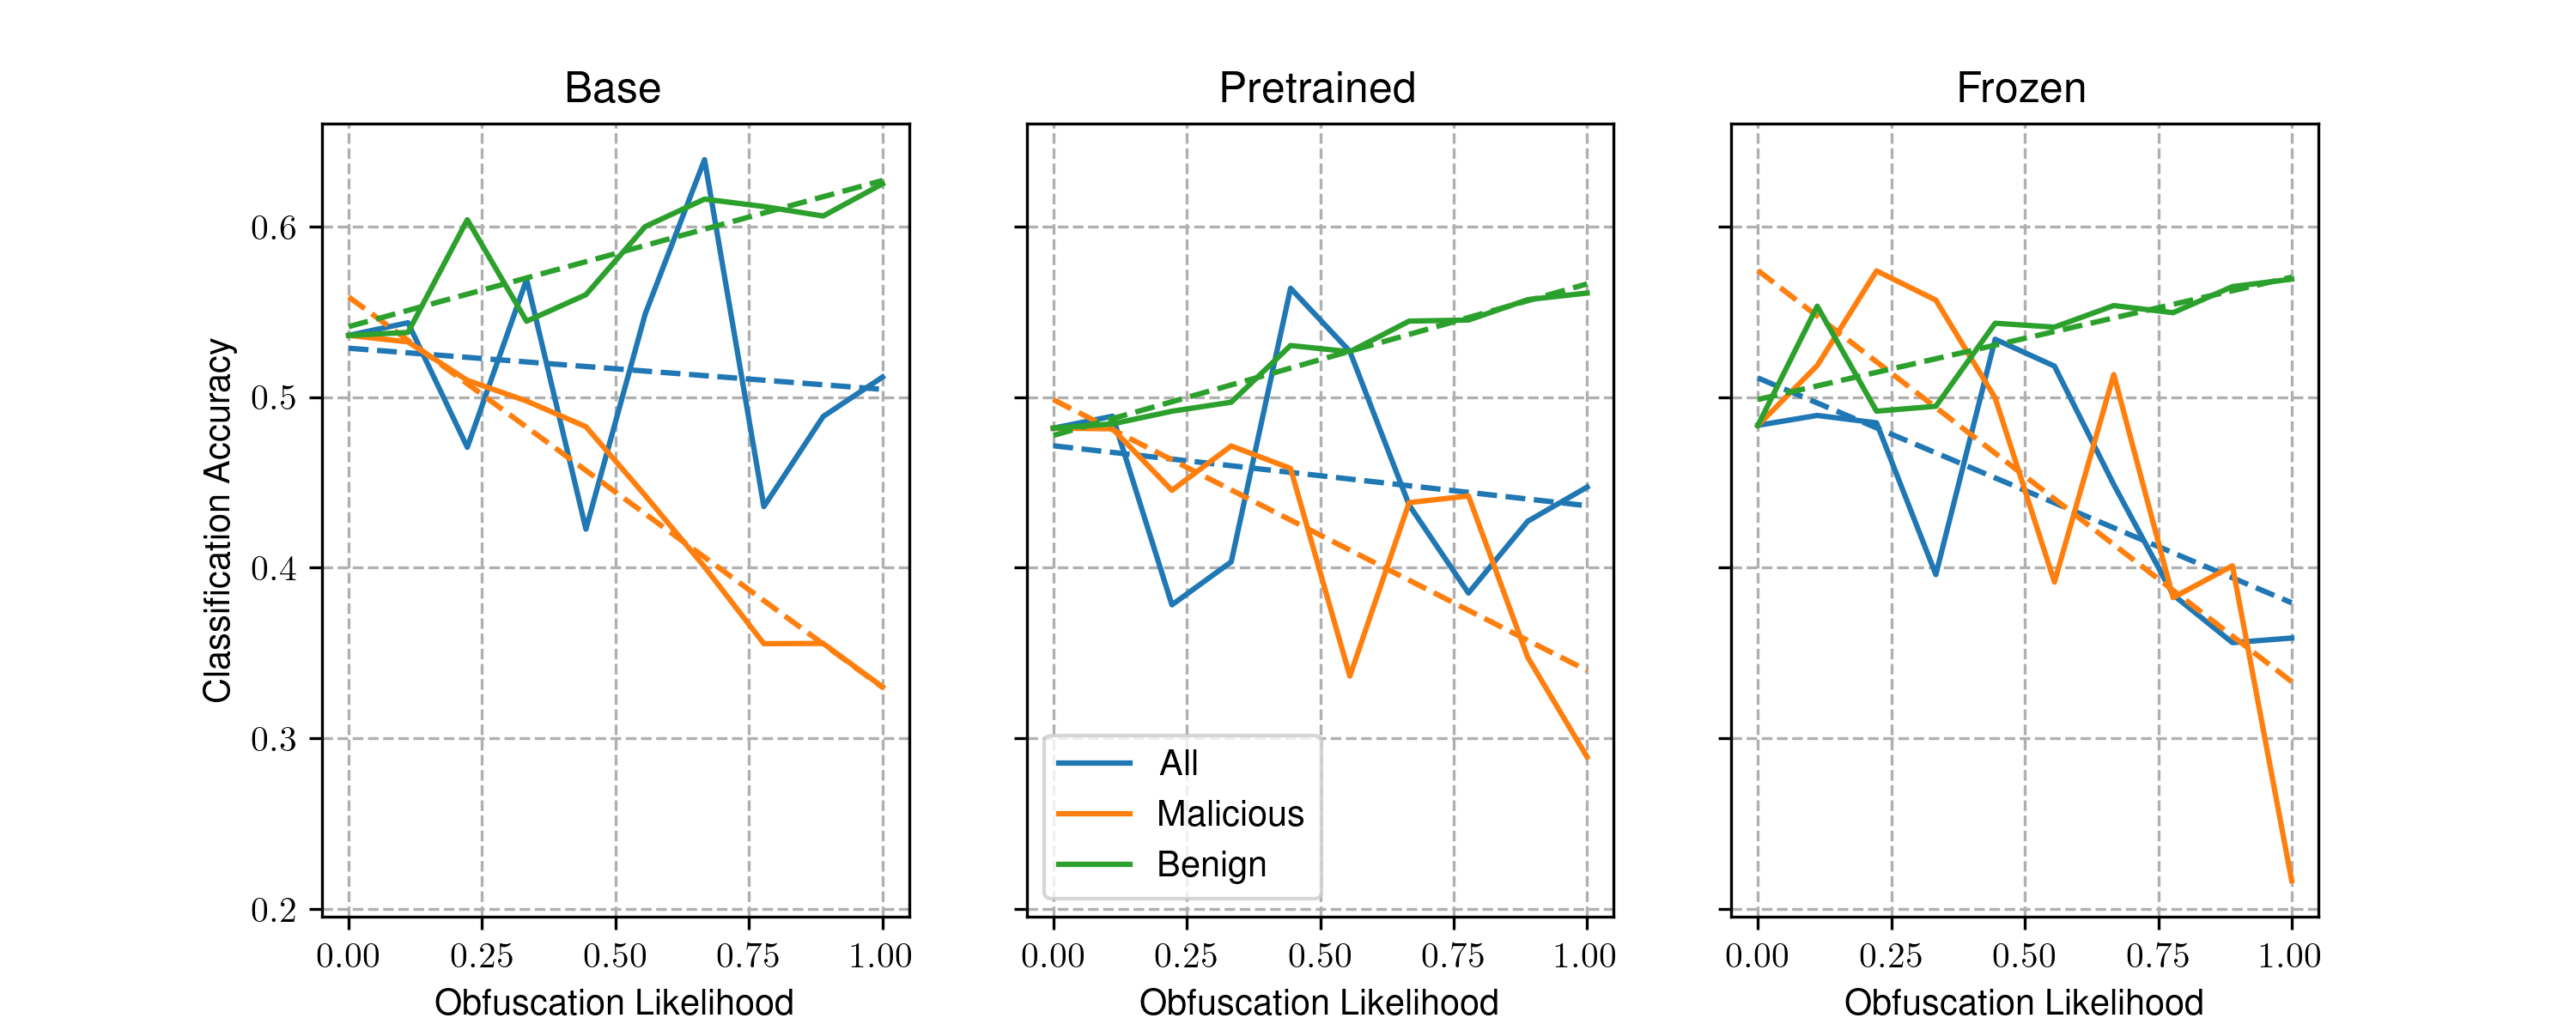
\includegraphics[width=\textwidth]{seq-obf-seq-level-pob.png}
        \caption{Sequence-level performance}
    \end{figure} 
\end{frame}

\begin{frame}{Partially Obfuscated Benign Model}{Certainty}
    \begin{figure}
        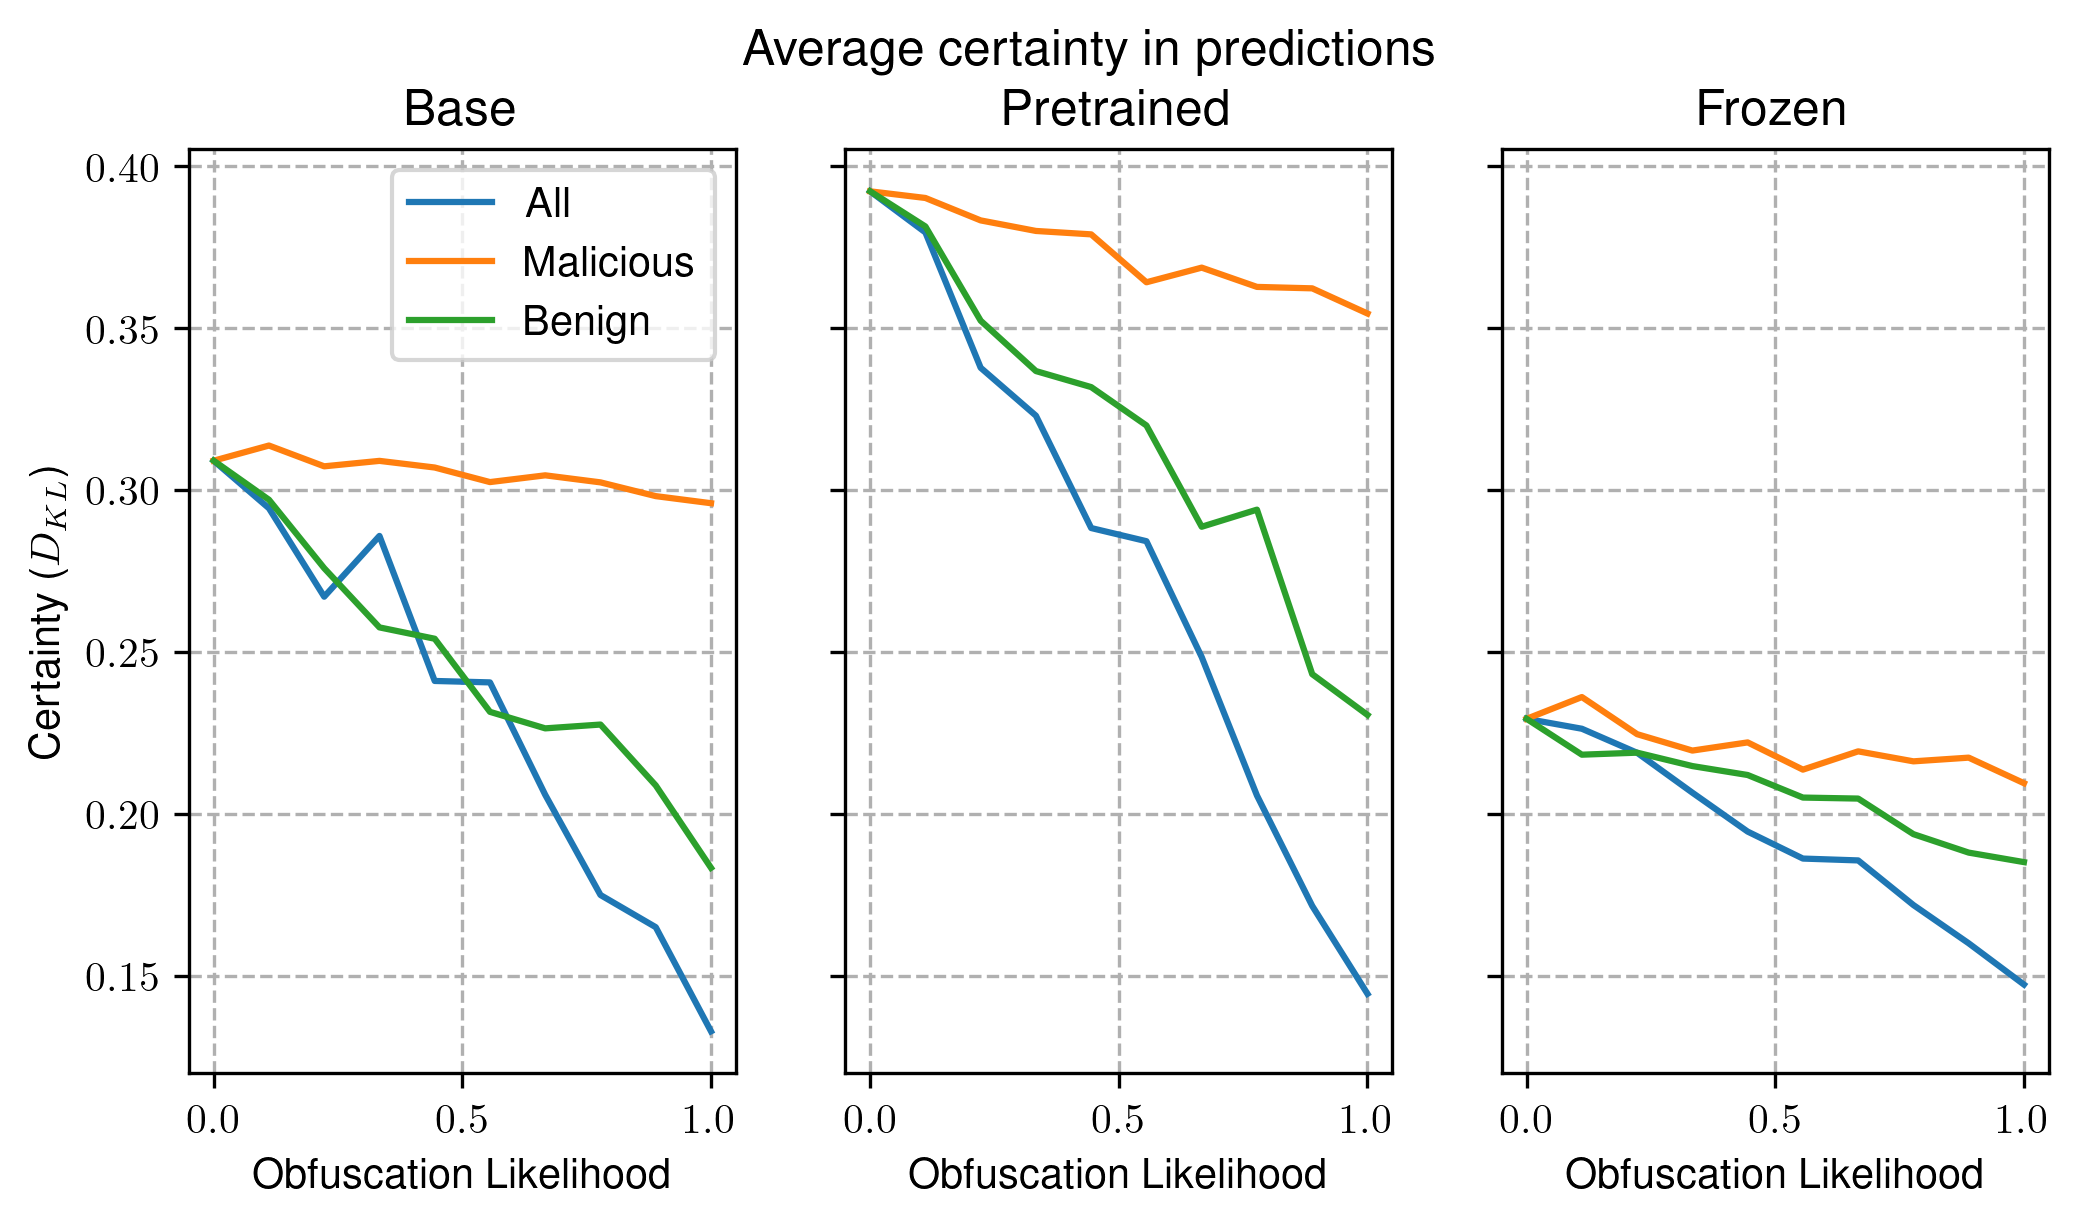
\includegraphics[width=\textwidth]{seq-obf-certainty-pob.png}
        \caption{Confidence}
    \end{figure} 
\end{frame}

\begin{frame}{Partially Obfuscated Benign Model}{RSA of Pretrained and Non-Pretrained Models}
    \begin{figure}
        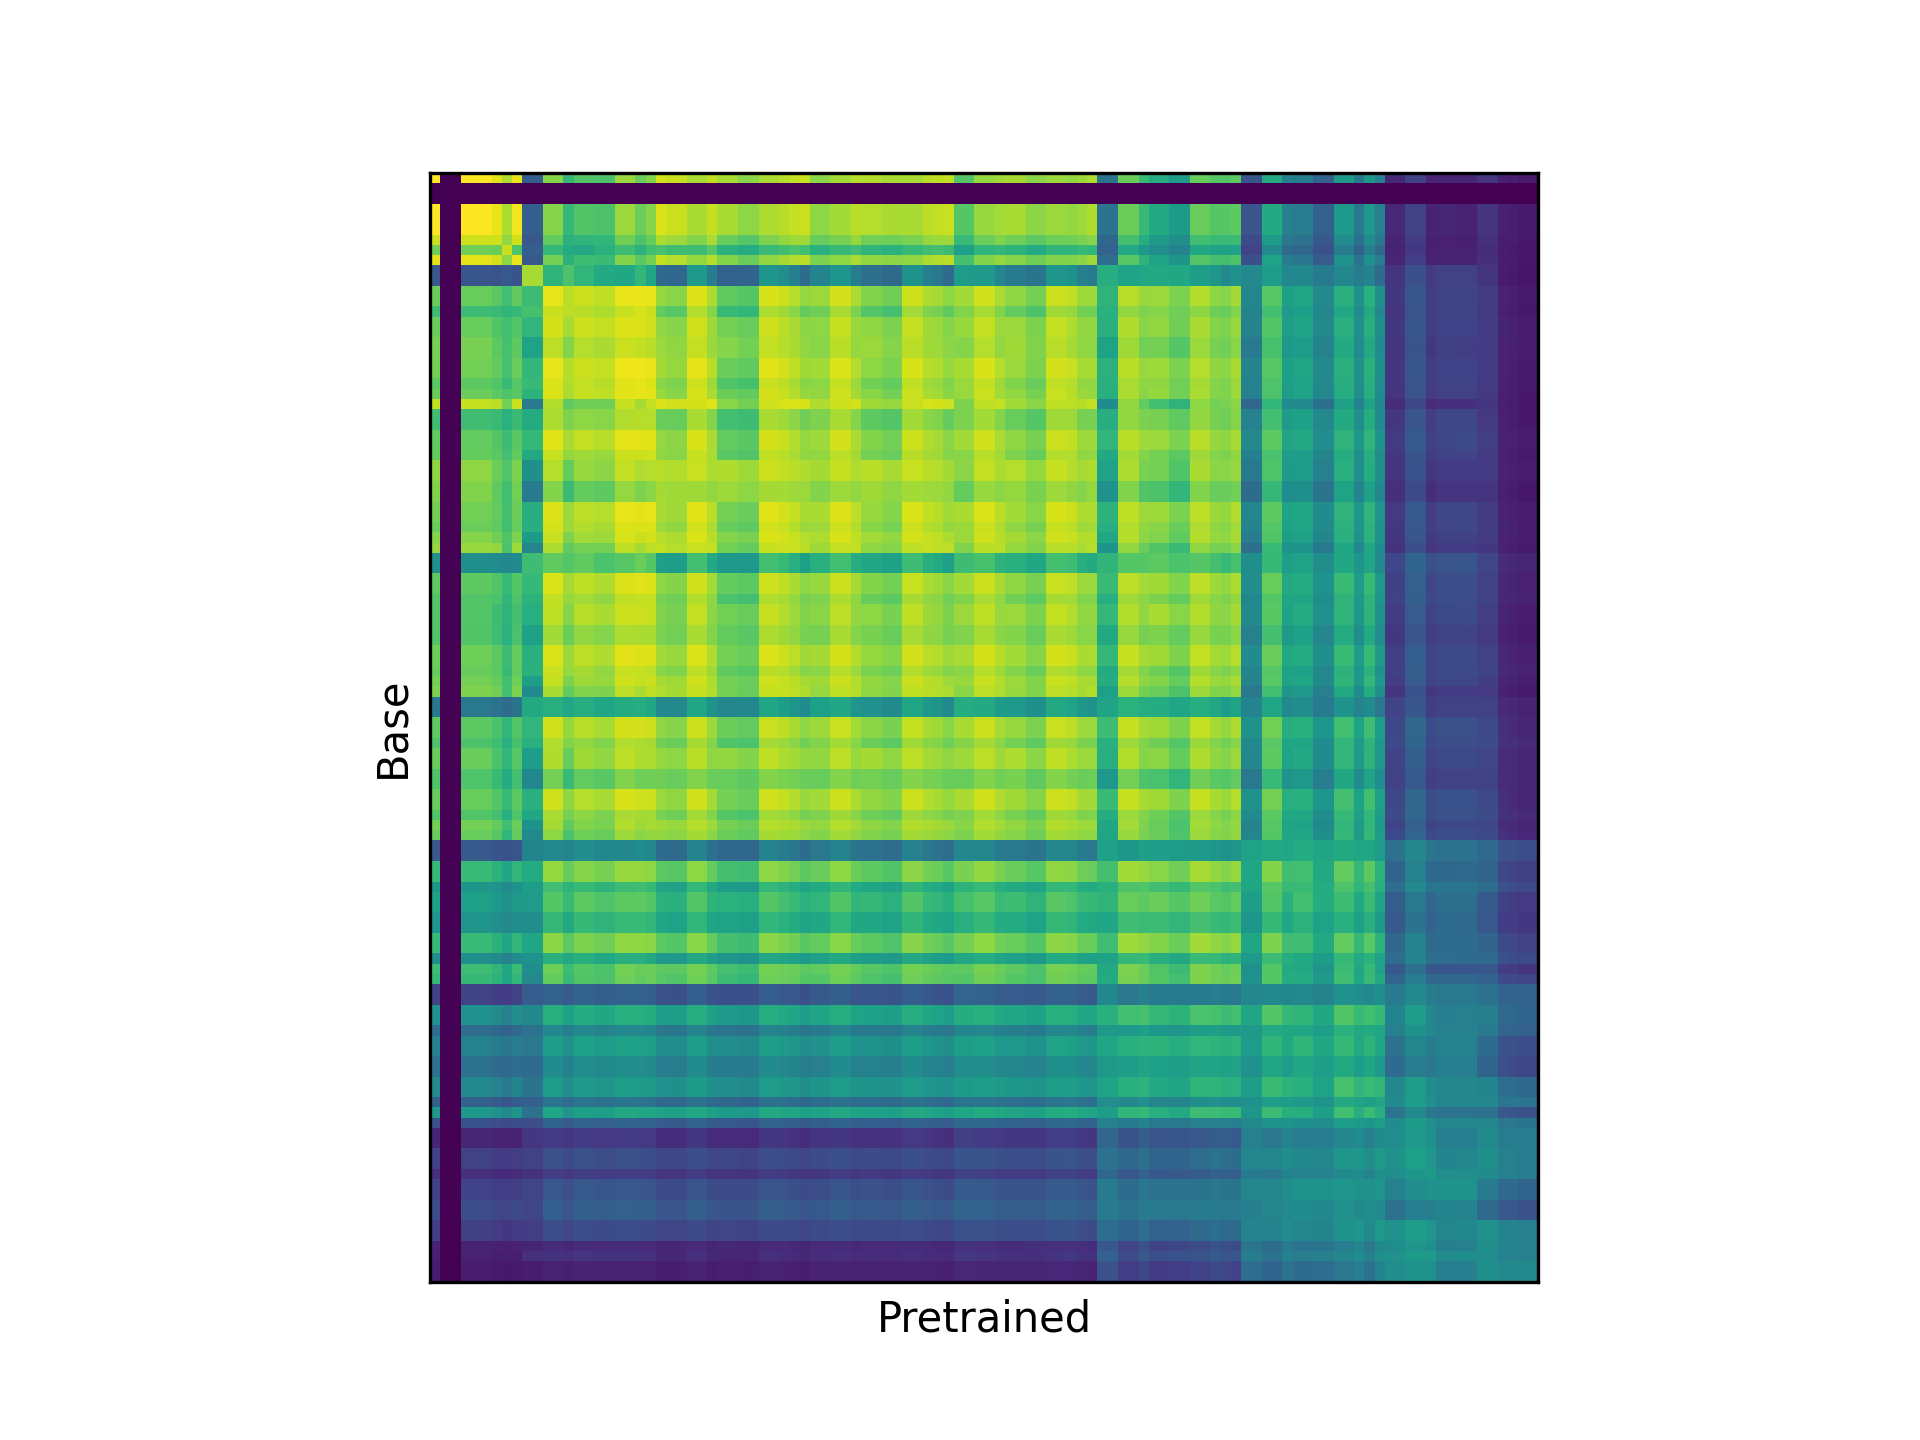
\includegraphics[width=0.5\textwidth]{rsa-cka-pob-pretrained-scratch.png}
    \end{figure}
\end{frame}

\begin{frame}{Partially Obfuscated Benign Model}{RSA of Pretrained and Frozen Pretrained Models}
    \begin{figure}
        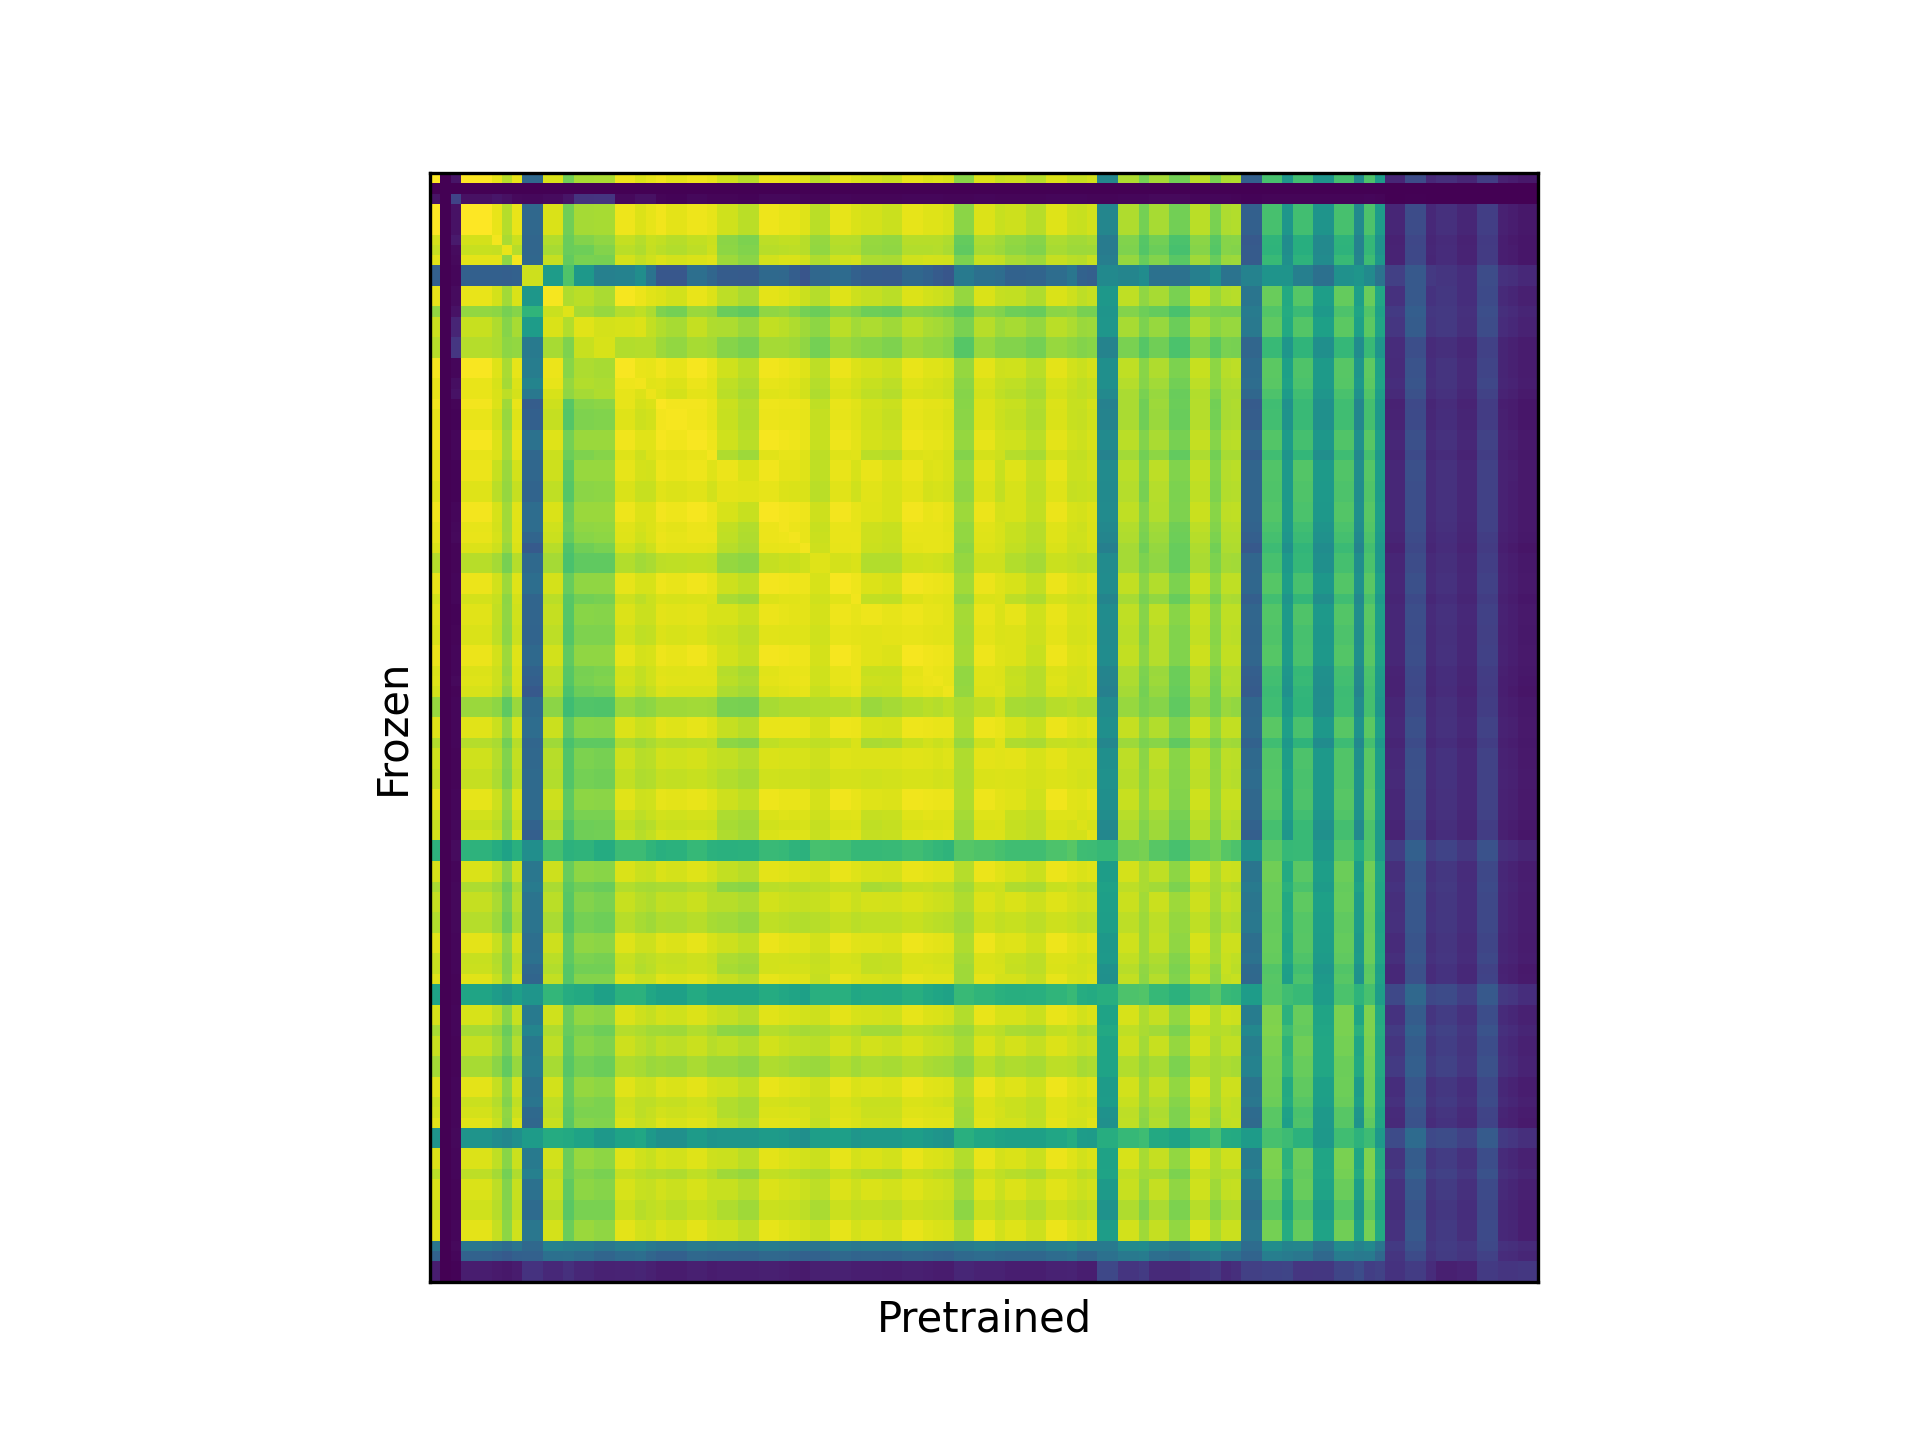
\includegraphics[width=0.5\textwidth]{rsa-cka-pob-pretrained-frozen.png}
    \end{figure}
\end{frame}
\begin{frame}{Partially Obfuscated Benign Model}{RSA of Frozen Pretrained and Non-Pretrained Models}
    \begin{figure}
        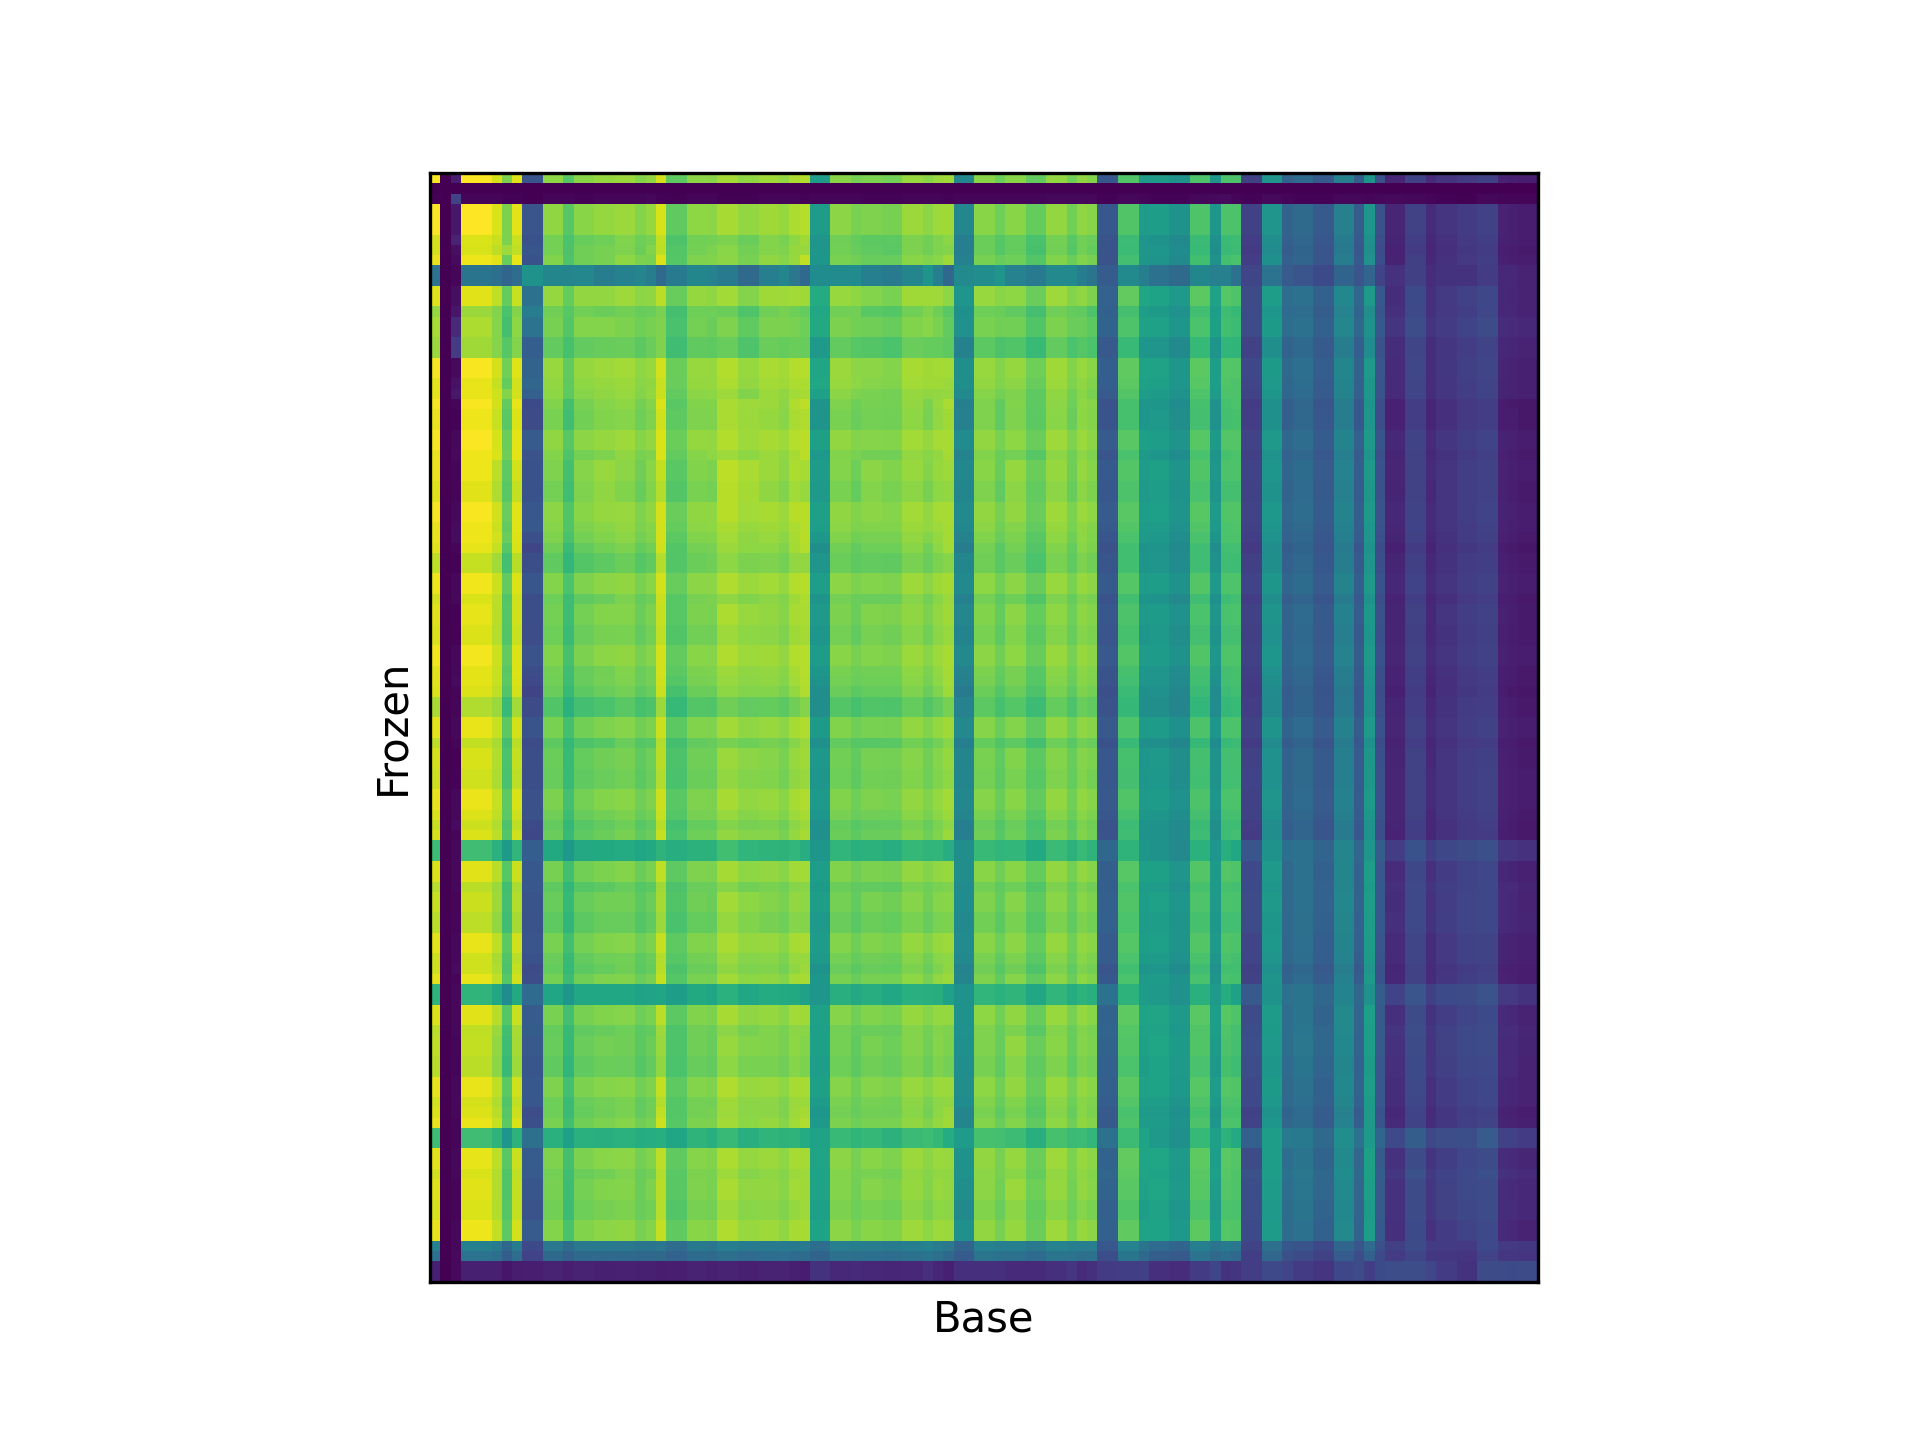
\includegraphics[width=0.5\textwidth]{rsa-cka-pob-frozen-scratch.png}
    \end{figure}
\end{frame}

\begin{frame}{Obfuscation Metric}{Entropy}
    \begin{figure}
        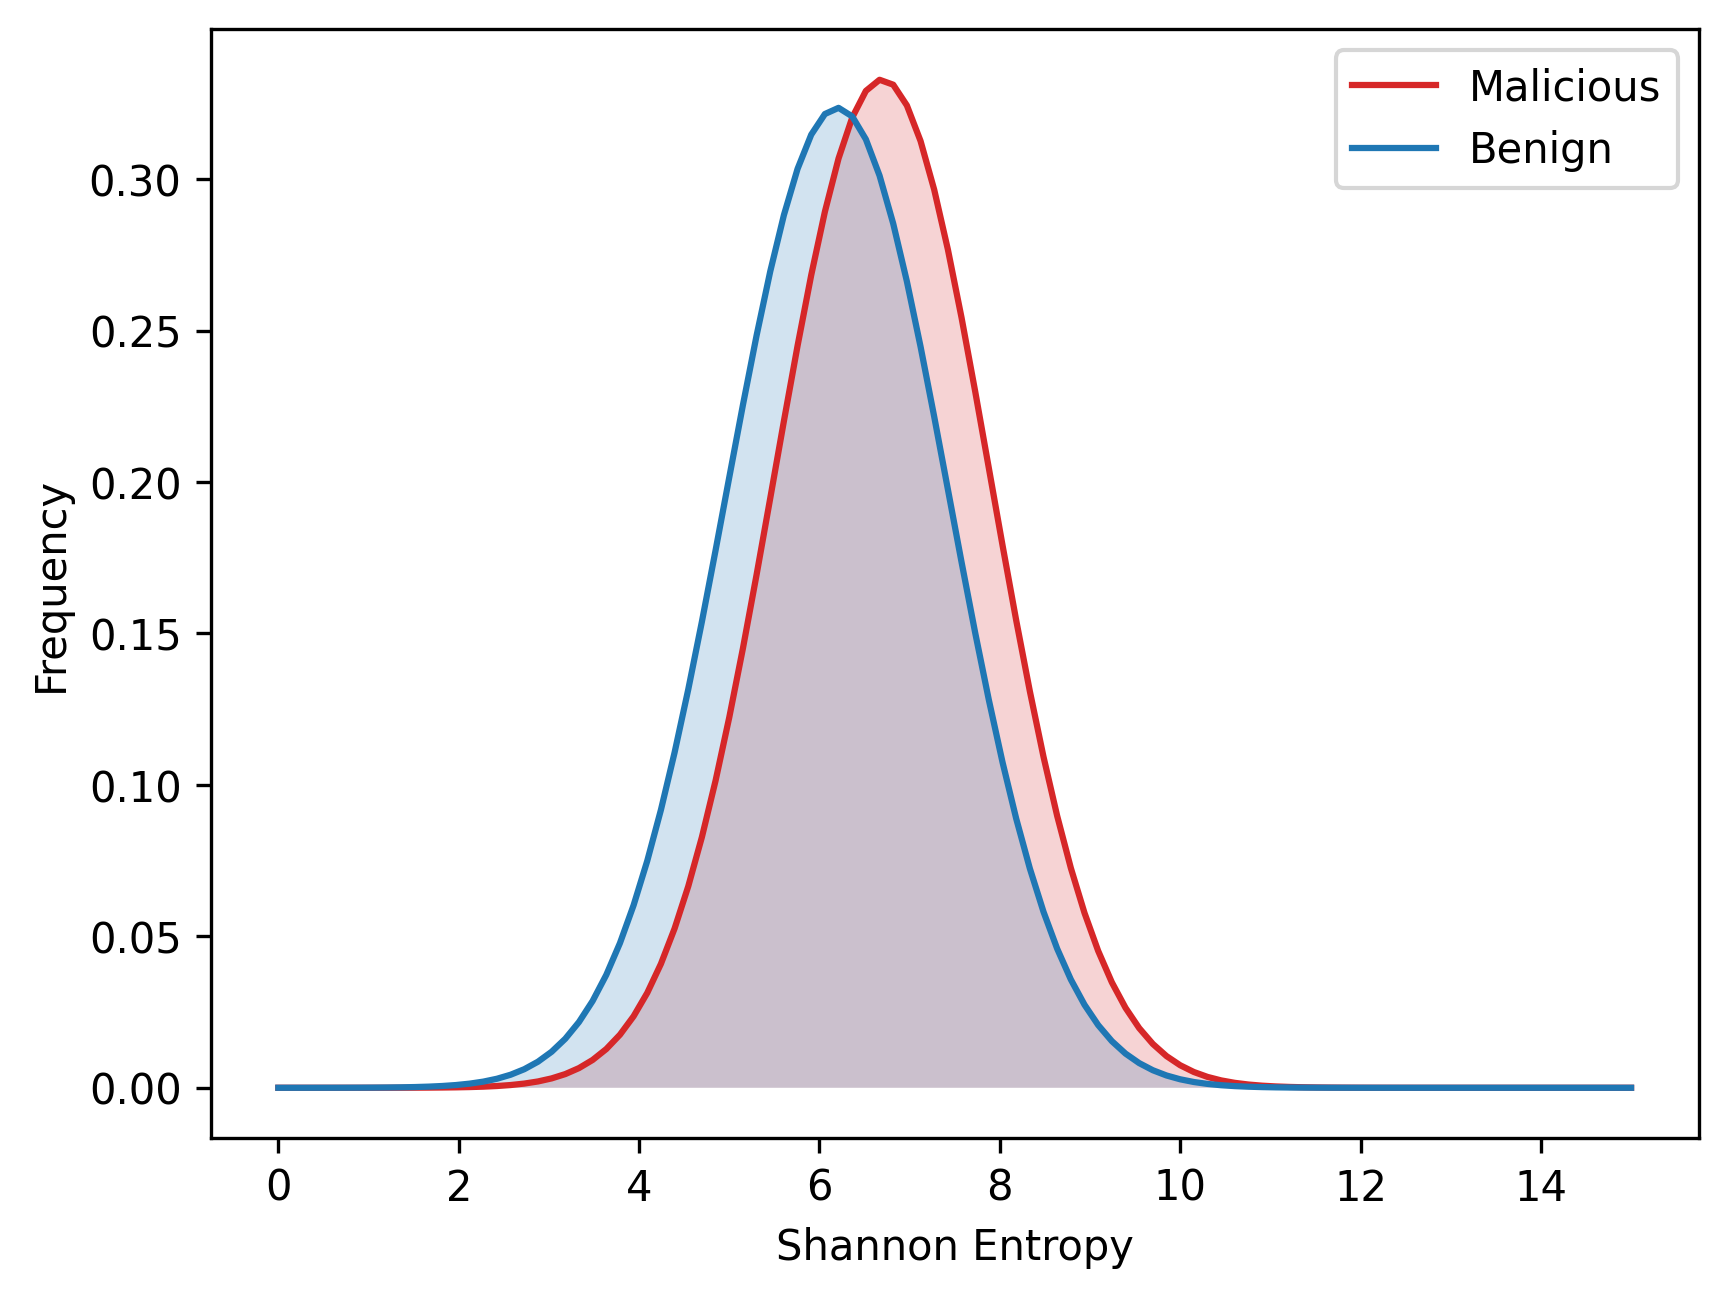
\includegraphics[width=0.5\textwidth]{entropy.png}
        \caption{Distribution of entropy for malicious and benign samples}
    \end{figure}
\end{frame}

\begin{frame}{Windows PE File Structure}
    \begin{figure}
        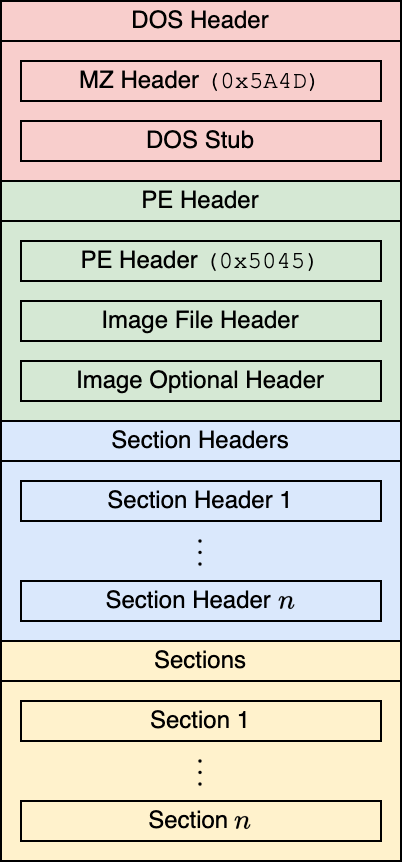
\includegraphics[scale=0.2]{pe.png}
    \end{figure} 
\end{frame}

\begin{frame}{Secondary Dataset --- Analysis Coverage}
    \begin{figure}
        
    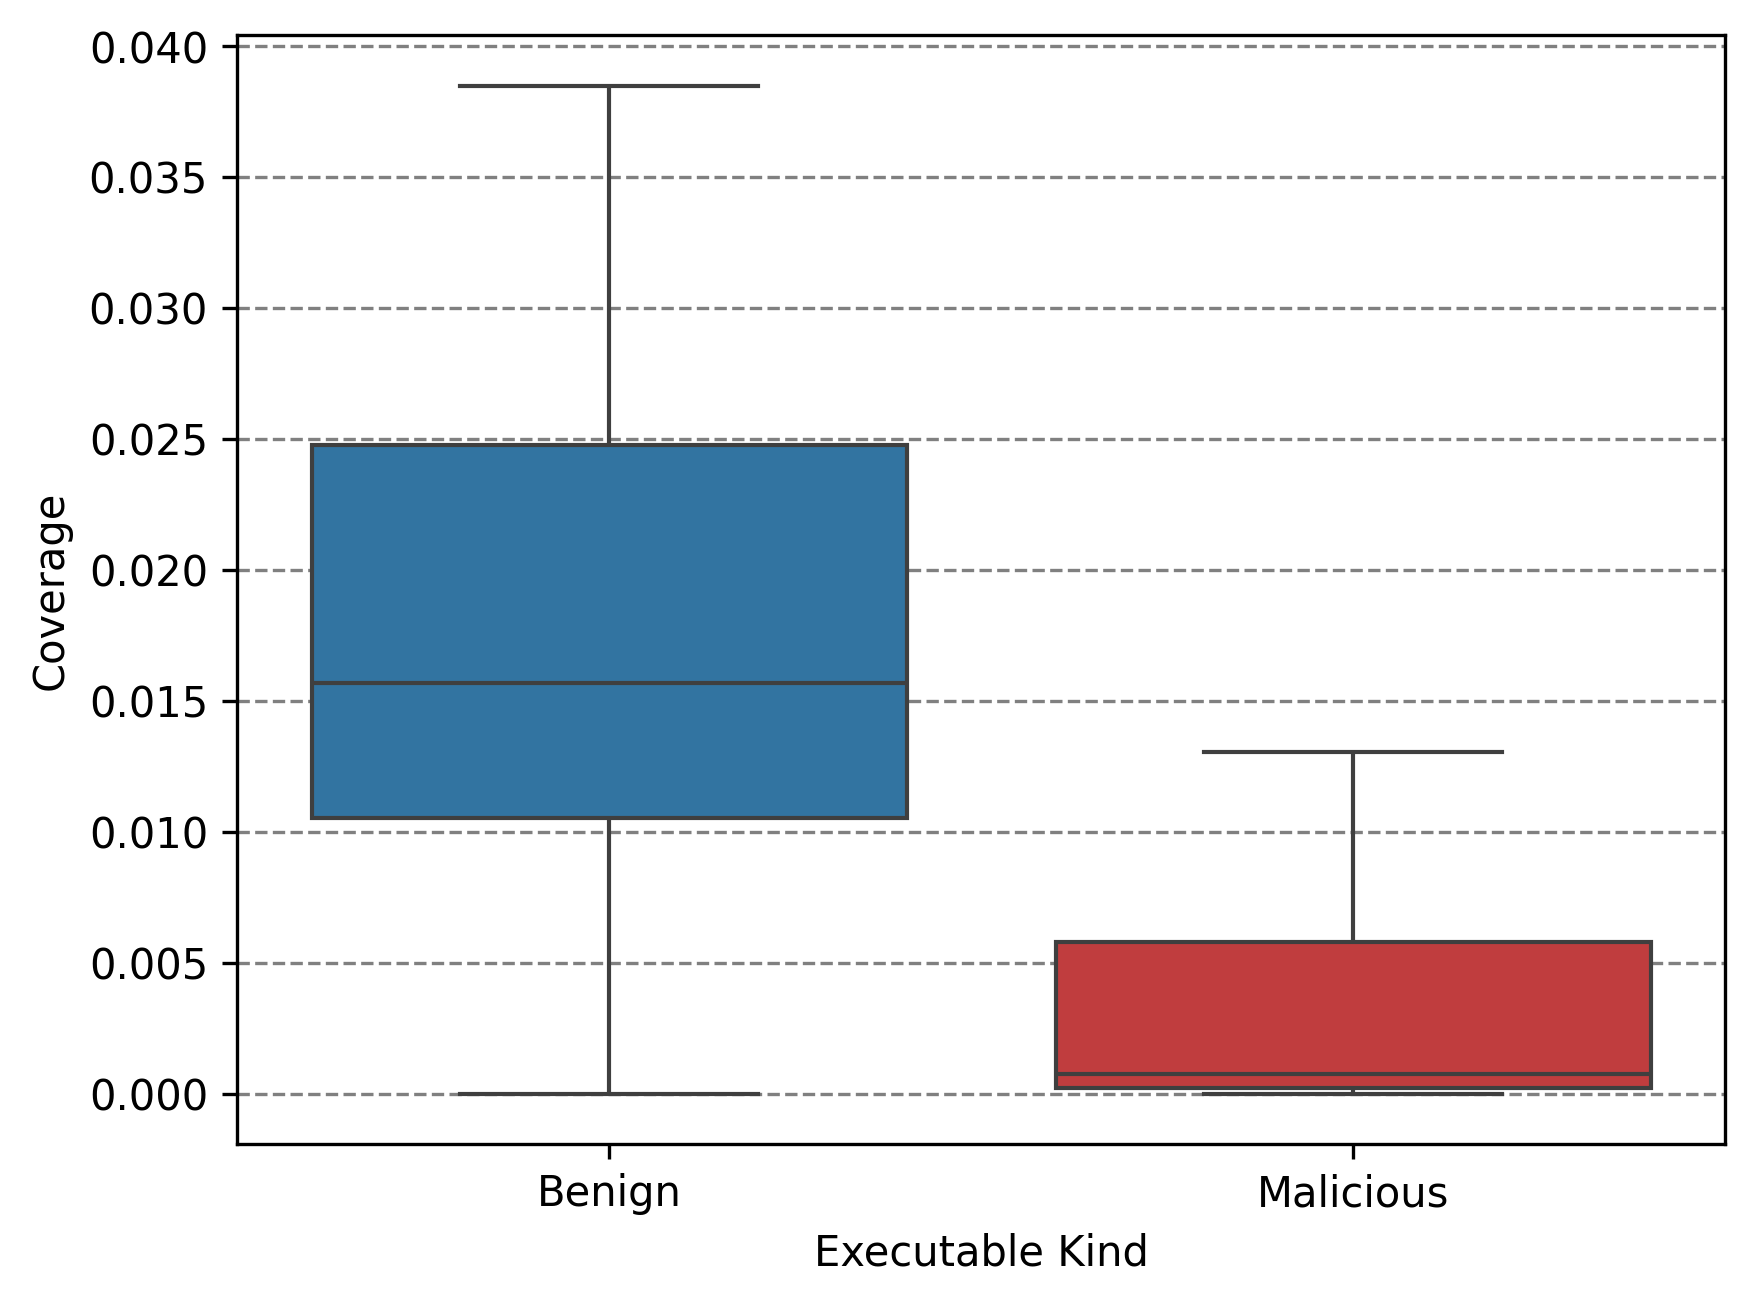
\includegraphics[scale=0.7]{obfuscation-dist-secondary-ds.png} 
    \end{figure}
\end{frame}
}
\end{document}